
%
%%%%%%%%%%%%%%%%%%%%%%%%%%%%%%%%%%%%%%%%%%%%%%%
%                                             %
% Seewald PhD thesis Latex source main file   %
% use: latexmk -pdf seewald2021.tex           %
% to generate the source                      %
%                                             %
%%%%%%%%%%%%%%%%%%%%%%%%%%%%%%%%%%%%%%%%%%%%%%%
%
\documentclass[10pt]{book}

\newcommand{\authorname}{Adam Seewald}
\newcommand{\booktitle}{Energy-Aware Coverage Planning and Scheduling for Autonomous Aerial Robots}  
\newcommand{\publisher}{University of Southern Denmark}
\newcommand{\editionyear}{2021}

\newcommand{\place}{Odense, Denmark}
\title{\booktitle}
\author{\authorname}

\usepackage{misc/options}


%%%%%%%%%%%%%%%%
%              %
% Glossaries   %
%              %
\newglossaryentry{not:exists}{
    type=notation,
    name={$\exists$},
    description={there exists}
}

\newglossaryentry{acr:lp}{
    type=acronym,
    name={LP},
    description={linear program}
}

\newglossaryentry{acr:qp}{
    type=acronym,
    name={QP},
    description={quadratic program}
}

\newglossaryentry{acr:mpc}{
    type=acronym,
    name={MPC},
    description={model predictive control}
}

\newglossaryentry{acr:nlp}{
    type=acronym,
    name={NLP},
    description={non linear program}
}

\newglossaryentry{acr:uav}{
    type=acronym,
    name={UAV},
    description={unmanned aerial vehicle}
}

\newglossaryentry{acr:uas}{
    type=acronym,
    name={UAS},
    description={unmanned aerial system}
}

\newglossaryentry{acr:ocp}{
    type=acronym,
    name={OCP},
    description={optimal control problem}
}

\newglossaryentry{acr:bvp}{
    type=acronym,
    name={BVP},
    description={boundary-value problem}
}

\newglossaryentry{acr:rsta}{
    type=acronym,
    name={RSTA},
    description={reconnaissance, surveillance, and target acquisition}
}

\newglossaryentry{acr:gnss}{
    type=acronym,
    name={GNSS},
    description={global navigation satellite system}
}

\newglossaryentry{acr:imu}{
    type=acronym,
    name={IMU},
    description={inertial measurement unit}
}

\newglossaryentry{acr:rpv}{
    type=acronym,
    name={RPV},
    description={remotely piloted vehicle}
}

\newglossaryentry{acr:gps}{
    type=acronym,
    name={GPS},
    description={global positioning system}
}
\makeglossaries

\makeindex
\usepackage[totoc]{idxlayout}

\addbibresource{backmatter/references.bib}

\begin{document}

%%%%%%%%%%%%%%%%%
                %
% Frontmatter   %
                %
\frontmatter

%%%%%%%%%%%%%%%%
%              %
% Title page   %
%              %
\pagestyle{empty}
{
\centering
	{\large ~\par}
	~

	\vspace{64pt}
	{\Huge\fontfamily{phv}\selectfont\bfseries\booktitle\par}

}
\cleardoublepage


\begin{titlepage}
	\centering
	{\large \publisher\par}
	~

	\vspace{64pt}
	{\Huge\fontfamily{phv}\selectfont\bfseries\booktitle\par}

	\vspace{6pt}
	\vspace{\stretch{1.25}}
	{\large A Dissertation submitted in partial satisfaction of the\par
	requirements for the degree of Doctor of Philosophy\par 
	in Robotics\par}
	
	\vspace{12pt}
	{\large\itshape by\par}
	
	\vspace{6pt}
	{\Large\itshape \authorname\par}

	\vspace{24pt}
	{\normalsize\begin{flushleft}{\itshape Approved by:}
		\begin{multicols}{2}
			{Dr. Ulrik Pagh Schultz, Advisor\\
			Unmanned Aerial Systems Center\\
			University of Southern Denmark
			}\par
			\columnbreak
			{~\\
			~\\
			~}\par
		\end{multicols}
		\vspace{6pt}
		\begin{multicols}{2}
		~\\\columnbreak {\itshape Approved on: }
		\end{multicols}	
	\end{flushleft}}

	\vspace{\stretch{6}}
	{\large \editionyear{}}
\end{titlepage}



%%%%%%%%%%%%%%%%%%%%
%                  %
% Copyright page   %
%                  %
{\small\setlength{\parindent}{0em}\setlength{\parskip}{1em}
~

\vfill

\url{https://doi.org/10.}

The typesetting is done using \LaTeX. Figures are generated with PGF/TikZ. Fonts are EB Garamond, Helvetica, and Iwona for body, headers, and equations respectively.

Copyright \copyright{} 2021 by \authorname. Some rights reserved.

This work is subject CC BY-NC-SA license, which means that you can copy, redistribute, remix, transform, and build upon the content for any non commercial purpose, as long as you give appropriate credit, provide a link to the license, and indicate if changes were made. If you remix, transform, or build upon the material, you must distribute your contributions under the same license as the original. License details: \url{https://creativecommons.org/licenses/by-nc-sa/4.0/}

\includegraphics[width=.2\textwidth]{by-nc-sa}

First edition, \editionyear{}

%ISBN \isbn{} 

Published by \publisher{}, in \place{}
}\cleardoublepage

% dedication
\pagestyle{empty} 
\thispagestyle{empty}
\vspace*{\fill}
\begin{chapquote}{\cite{wright1913how}}
    \noindent ``[I]t was not possible to run it more than a minute or two at a time. In these short tests the motor developed about nine horse power. We were then satisfied that, with proper lubrication and better adjustments, a little more power could be expected.''
\end{chapquote}
\vspace*{\fill}
\cleardoublepage
\pagestyle{fancy}

%
%%%%%%%%%%%%%%%%%%%%%%
%                    %
% Acknowledgements   %
%                    %
%%%%%%%%%%%%%%%%%%%%%%
%
% PASS
%
\chapter*{Acknowledgements}

%\lettrine{A}{a}

I am obliged to my advisor Prof. Ulrik Pagh Schultz for his encouragement, patience, and helpful discussions. He was always ready with a very thorough list of insightful suggestions and improvements. My gratitude goes also to my co-advisors, Dr. H\'ector Garc\'ia de Marina, who proposed the direction of this work, and Dr. Henrik Skov Midtiby, who shaped the outcomes.

Parts of this work are a result of collaborative efforts. I am indebted to Julius Roeder, Dr. Benjamin Rouxel, and Dr. Clemens Grelck from the Parallel Computing Systems group at the University of Amsterdam and to my colleagues, past and present, from the Unmanned Aerial Systems group at the University of Southern Denmark. I am additionally grateful to TeamPlay project consortium members for stimulating debates on low power computing during various occasions.

Finally, I wish to thank my mother and maternal grandparents who were of great support and indulgence.

\cleardoublepage   % tocpage on right-side

\thispagestyle{empty} 
\pagestyle{fancy}\tableofcontents\cleardoublepage\thispagestyle{empty} % toc
\renewcommand{\numberline}[1]{\hspace*{-1.5em}}
\pagestyle{fancy}\listoffigures\cleardoublepage\thispagestyle{empty} % list of figures
\pagestyle{fancy}\printunsrtglossary[type=notation,style=long]\cleardoublepage\thispagestyle{empty} % notation
\pagestyle{fancy}\printunsrtglossary[type=acronym,style=long]\cleardoublepage\thispagestyle{empty} % acronyms


%%%%%%%%%%%%%%%%
               %
% Mainmatter   %
               %
\mainmatter
\pagestyle{fancy}

%%%%%%%%%%%%%%%%%%
%                %
% Introduction   %
%                %
\chapter{Introduction}
\lettrine{L}{orem ipsum dolor sit amet}, consectetuer adipiscing elit. Etiam lobortis facilisis sem. Nullam nec mi et neque pharetra sollicitudin. Praesentimperdiet mi nec ante. Donec ullamcorper, felis non sodales commodo, lectus velit ultrices augue, a dignissim nibh lectus placerat pede. Vivamus nunc nunc, molestie ut, ultricies vel, semper in, velit. Ut porttitor. Praesent in sapien. Lorem ipsum dolor sit amet, consectetuer adipiscing elit. Duis fringilla tristique neque. Sed interdum libero ut metus. Pellentesque placerat. Nam rutrum augue a leo. Morbi sed elit sit amet antelobortis sollicitudin. Praesent blandit blandit mauris. Praesent lectustellus, aliquet aliquam, luctus a, egestas a, turpis. Mauris lacinia loremsit amet ipsum. Nunc quis urna dictum turpis accumsan semper.

\begin{equation}
    \sin x = \sum\limits_{n = 1}^\infty  {\frac{{\left( { - 1} \right)^{n - 1} x^{2n - 1} }}{{\left( {2n - 1} \right)!}}}
\end{equation} % test equation

\section{A Test Section}

Lorem ipsum dolor sit amet, consectetuer adipiscing elit. Etiam lobortis facilisis sem. Lorem ipsum dolor sit amet~\citep{seewald2020beyond}, consectetuer adipiscing elit. Etiam lobortis facilisis sem. Nullam nec mi et neque pharetra sollicitudin. Praesentimperdiet mi nec ante. Donec ullamcorper, felis non sodales commodo, lectus velit ultrices augue, a dignissim nibh lectus placerat pede. Vivamus nunc nunc, molestie ut, ultricies vel, semper in, velit. Ut porttitor. Praesent in sapien. Lorem ipsum dolor sit amet, consectetuer adipiscing elit. Duis fringilla tristique neque. Sed interdum libero ut metus. Pellentesque placerat. Nam rutrum augue a leo. Morbi sed elit sit amet antelobortis sollicitudin. Praesent blandit blandit mauris. Praesent lectustellus, aliquet aliquam, luctus a, egestas a, turpis. Mauris lacinia loremsit amet ipsum. Nunc quis urna dictum turpis accumsan semper. % citation test

\subsection{A test subsection 1}

\begin{figure}[t]
    \centering
    \includegraphics[width=.8\textwidth]{photo}
    \caption[A test short title]{A test long title. Vivamus nunc nunc, molestie ut, ultricies vel, semper in, velit. Ut porttitor. Praesent in sapien. Lorem ipsum dolor sit amet, consectetuer adipiscing elit. Duis fringilla tristique neque. Sed interdum libero ut metus. Pellentesque placerat. Nam rutrum augue a leo. Morbi sed elit sit amet antelobortis sollicitudin. Praesent blandit blandit mauris.}
\end{figure}

Lorem ipsum dolor sit amet, consectetuer adipiscing elit. Etiam lobortis facilisis sem. Nullam nec mi et neque pharetra sollicitudin. Praesentimperdiet mi nec ante. Donec ullamcorper, felis non sodales commodo, lectus velit ultrices augue, a dignissim nibh lectus placerat pede. Vivamus nunc nunc, molestie ut, ultricies vel, semper in, velit. Ut porttitor. Praesent in sapien. Lorem ipsum dolor sit amet, consectetuer adipiscing elit. Duis fringilla tristique neque. Sed interdum libero ut metus. Pellentesque placerat. Nam rutrum augue a leo. Morbi sed elit sit amet antelobortis sollicitudin. Praesent blandit blandit mauris. Praesent lectustellus, aliquet aliquam, luctus a, egestas a, turpis. Mauris lacinia loremsit amet ipsum. Nunc quis urna dictum turpis accumsan semper.

Lorem ipsum dolor sit amet, consectetuer adipiscing elit. Etiam lobortis facilisis sem. Nullam nec mi et neque pharetra sollicitudin. Praesentimperdiet mi nec ante. Donec ullamcorper, felis non sodales commodo, lectus velit ultrices augue, a dignissim nibh lectus placerat pede. Vivamus nunc nunc, molestie ut, ultricies vel, semper in, velit. Ut porttitor. Praesent in sapien. Lorem ipsum dolor sit amet, consectetuer adipiscing elit. Duis fringilla tristique neque. Sed interdum libero ut metus. Pellentesque placerat. Nam rutrum augue a leo. Morbi sed elit sit amet antelobortis sollicitudin. Praesent blandit blandit mauris. Praesent lectustellus, aliquet aliquam, luctus a, egestas a, turpis. Mauris lacinia loremsit amet ipsum. Nunc quis urna dictum turpis accumsan semper.

\subsection{A test subsection 2}

Lorem ipsum dolor sit amet, consectetuer adipiscing elit. Etiam lobortis facilisis sem. Nullam nec mi et neque pharetra sollicitudin. Praesentimperdiet mi nec ante. Donec ullamcorper, felis non sodales commodo, lectus velit ultrices augue, a dignissim nibh lectus placerat pede. Vivamus nunc nunc, molestie ut, ultricies vel, semper in, velit. Ut porttitor. Praesent in sapien. Lorem ipsum dolor sit amet, consectetuer adipiscing elit. Duis fringilla tristique neque. Sed interdum libero ut metus. Pellentesque placerat. Nam rutrum augue a leo. Morbi sed elit sit amet antelobortis sollicitudin. Praesent blandit blandit mauris. Praesent lectustellus, aliquet aliquam, luctus a, egestas a, turpis. Mauris lacinia loremsit amet ipsum. Nunc quis urna dictum turpis accumsan semper.

Lorem ipsum dolor sit amet, consectetuer adipiscing elit. Etiam lobortis facilisis sem. Nullam nec mi et neque pharetra sollicitudin. Praesentimperdiet mi nec ante. Donec ullamcorper, felis non sodales commodo, lectus velit ultrices augue, a dignissim nibh lectus placerat pede. Vivamus nunc nunc, molestie ut, ultricies vel, semper in, velit. Ut porttitor. Praesent in sapien. Lorem ipsum dolor sit amet, consectetuer adipiscing elit. Duis fringilla tristique neque. Sed interdum libero ut metus. Pellentesque placerat. Nam rutrum augue a leo. Morbi sed elit sit amet antelobortis sollicitudin. Praesent blandit blandit mauris. Praesent lectustellus, aliquet aliquam, luctus a, egestas a, turpis. Mauris lacinia loremsit amet ipsum. Nunc quis urna dictum turpis accumsan semper.

Lorem ipsum dolor sit amet, consectetuer adipiscing elit. Etiam lobortis facilisis sem. Nullam nec mi et neque pharetra sollicitudin. Praesentimperdiet mi nec ante. Donec ullamcorper, felis non sodales commodo, lectus velit ultrices augue, a dignissim nibh lectus placerat pede. Vivamus nunc nunc, molestie ut, ultricies vel, semper in, velit. Ut porttitor. Praesent in sapien. Lorem ipsum dolor sit amet, consectetuer adipiscing elit. Duis fringilla tristique neque. Sed interdum libero ut metus. Pellentesque placerat. Nam rutrum augue a leo. Morbi sed elit sit amet antelobortis sollicitudin. Praesent blandit blandit mauris. Praesent lectustellus, aliquet aliquam, luctus a, egestas a, turpis. Mauris lacinia loremsit amet ipsum. Nunc quis urna dictum turpis accumsan semper.

Lorem ipsum dolor sit amet, consectetuer adipiscing elit. Etiam lobortis facilisis sem. Nullam nec mi et neque pharetra sollicitudin. Praesentimperdiet mi nec ante. Donec ullamcorper, felis non sodales commodo, lectus velit ultrices augue, a dignissim nibh lectus placerat pede. Vivamus nunc nunc, molestie ut, ultricies vel, semper in, velit. Ut porttitor. Praesent in sapien. Lorem ipsum dolor sit amet, consectetuer adipiscing elit. Duis fringilla tristique neque. Sed interdum libero ut metus. Pellentesque placerat. Nam rutrum augue a leo. Morbi sed elit sit amet antelobortis sollicitudin. Praesent blandit blandit mauris. Praesent lectustellus, aliquet aliquam, luctus a, egestas a, turpis. Mauris lacinia loremsit amet ipsum. Nunc quis urna dictum turpis accumsan semper.



%
%%%%%%%%%%%%%%%%%%%%%%%%%
%                       %
% Problem Formulation   %
%                       %
%%%%%%%%%%%%%%%%%%%%%%%%%
%
% Brief abstract: formulates the two problem (coverage, (re)planning)
%
% Completion (1-10): 10
% Missing: none, but further consistency check is needed
%
\chapter{Problem Formulation}
\label{cp:pb}

\begin{chapquote}{\cite{arkin2001optimal}}
  ``While we will often speak of the [coverage] problem as `milling' with a `cutter', many of its important applications arise in various contexts outside of machining.''
\end{chapquote}

\vspace*{1em}

\lettrine{I}{n this chapter}, we discuss the planning and coverage problems that we are interested in solving. The coverage problem is the problem of finding the path that covers all the points in a given space~\citep{choset2001coverage,galceran2013survey}, for instance, the agricultural field in \fref{sec:motivation}{Section}. The coverage path with some user-defined computations forms the plan. The planning problem is then the problem of replanning the plan. It is replanned energy-wise in the eventuality of energy constraints dissatisfaction, and whenever the uncertainty affects the flight unexpectedly. To define both the problems, we need some basic constructs. In particular, we provide formal definitions in \fref{sec:definitions}{Sections}\fref{sec:defs-stages-triggs}{--\hspace*{-.8ex}} that include the computations, motion, computations energy, and motion energy. We then define the difference between computations and motion energy (\Gls{acr:mace}), which we encountered in \fref{sec:aerial-robo-types}{Section}, path, and other plan-specific constructs. We then use all these to formulate the planning and coverage problems in \fref{sec:plan-pb}{Section}. We illustrate the problem with an example of the precision agriculture use case in \fref{sec:flight-plan}{Section}.

In \fref{cp:dyn}{Chapter}, we propose two algorithms. A first algorithm generates the coverage path, and another algorithm replans the plan in time, solving the coverage and planning problems. The replanning is energy-aware: the algorithm outputs the best trajectory of the path and computations alteration for an aerial robot with varying battery and atmospheric conditions. 

The chapter connects to the remainder of this work as follows. Here we formalize the plan, the planning and coverage problems, and some other basic constructs. We use the plan characteristics to derive an energy model in \fref{cp:model}{Chapter}. We solve the planning problem using modern optimal control techniques and the coverage problem using a coverage path planning (\Gls{acr:cpp})\findex{coverage path planning} algorithm in \fref{cp:dyn}{Chapter}. We guide the aerial robot using a vector field, using the plan's building blocks from this chapter. We show the solutions to the problems experimentally in \fref{cp:res}{Chapter}. We discuss past approaches to solve the problems in \fref{cp:soa}{Chapter} and the concrete implementation in \fref{app:imp}{Appendix}.



%---


%%%%%%%%%%%%%%%%%%%%%%%%%%%%%%%%%%%%%%%%%%%%%%%%
\section{Definitions of computations and motion}
\label{sec:definitions}

Firstly, we define computations, motion, their energy, and M\&CE. Our dynamic planning depends on these basic concepts.

\begin{defn}[Computations/motion]
  \label{def:comps}
  \emph{Computations}\findex{computations} are energy-demanding computational tasks. The aerial robot runs the computations on heterogeneous computing hardware that interfaces microcontrollers.
  \emph{Motion}\findex{motion} is the act of the aerial robot moving in the surrounding environment. The aerial robot runs some primitives on microcontrollers that interface actuators, motors, and other components.
\end{defn}

Autonomous capabilities are often achieved by interconnecting heterogeneous computing hardware and microcontrollers. We assume for the computations that the heterogeneous computing hardware runs a schedule parametrized by some parameters. For instance, for the CNN detection from the precision agriculture scenario in \fref{sec:objective}{Section}, a parameter is the frames per second (\Gls{acr:fps})\findex{frames per second} rate. Alike for the computations, we assume for the motion that the robot travels some paths parametrized by some other parameters. For instance, for the coverage, a parameter changes the distance between the survey lines.

\begin{defn}[Computations/motion and overall energy]
  \label{def:comp-mot-energy}
  Given a path parametrized by $\rho$ parameters $c_i^\rho:=\{c_{i,1},c_{i,2},\dots,c_{i,\rho}\}$, the \emph{motion energy}\findex{motion energy} is the energy spent by the aerial robot while moving on the path.
  Given a schedule parametrized by parameters $c_i^\sigma:=\{c_{i,\rho+1},c_{i,\rho+2},\dots,c_{i,\rho+\sigma}\}$, the \emph{computations energy}\findex{computations energy} is the energy spent by heterogeneous computing hardware executing the schedule.
  The \emph{overall energy}\findex{overall energy} is the sum of motion energy and computations energy.
\end{defn}

Physically, motion energy is the energy spent by all the systems powering the aerial robot, excluding the heterogeneous computing hardware. We use watts for instantaneous or average measures of computations, motion, and overall energies, whereas joules for measures over a given time interval. We show in \fref{sec:defs-stages-triggs}{Section} what we mean by the parametrization of paths and computations with some parameters.

\Gls{acr:mace}\findex{difference of motion and computations energy} that we introduced in \fref{sec:aerial-robo-types}{Section} is the difference between average motion and computations energy. It is measured in watts, and it gives a measure of which of the two energy components is predominant. For \Gls{acr:mace} greater than zero, the motion energy dominates over the computations. The dynamic planning approach plans first an energy-efficient path. If we return briefly to \fref{fig:robots-vs-power}{Figure}, it is the case for rotary-wing aerial robots \sref{lab:matrice} and \sref{lab:agras}. On the contrary, for \Gls{acr:mace} lower than zero, the computations energy dominates. The dynamic planning approach plans first a power-saving schedule. It is the case for the lighter-than-air aerial robot \sref{lab:skye} in \fref{fig:robots-vs-power}{Figure}. For \Gls{acr:mace} close to zero, both energy components are important energy-wise. The dynamic planning approach plans both an energy-efficient path and a power-saving schedule to a similar extent. This M\&CE is characteristic of fixed-wing aerial robots, such as \sref{lab:cumulus}\fref{lab:opterra}{--\hspace*{-.8ex}} in \fref{fig:robots-vs-power}{Figure}.


%%%%%%%%%%%%%%%%%%%%%%%%%%%%%%%%%%%%%%
\section{Definition of path functions}
\label{sec:path-functions}

To model the path, we use multiple mathematical functions $\varphi_1,\varphi_2,\dots$ that we call path functions. These functions express the path in 2D space at an altitude $h\in\mathbb{R}$ for an inertial navigation frame $\mathcal{O}_W$. We discuss a generalization of the path functions in 3D space and how it affects the guidance in \fref{cp:conc}{Chapter}. 

\begin{defn}[Path functions]
  \label{def:paths}
  $\varphi_i:\mathbb{R}^2\rightarrow\mathbb{R},\,\forall i\in\{1,2,\dots\}$ are \emph{path functions}\findex{path functions} used to model the path. They are a function of a generic time-dependent point $\mathbf{p}(t):=(x_{\mathbf{p}(t)},y_{\mathbf{p}(t)})$ of the aerial robot flying in the 2D space and are continuous and twice differentiable. 
\end{defn}

\begin{figure}[t!]
  \centering
  
\definecolor{cECECEC}{RGB}{236,236,236}
\definecolor{c989898}{RGB}{152,152,152}
\small

\def \globalscale {1.000000}
\begin{tikzpicture}[y=0.80pt, x=0.80pt, yscale=-.9*\globalscale, xscale=.9*\globalscale, inner sep=0pt, outer sep=0pt]
\path[fill=cECECEC,line join=round,line width=0.160pt] (338.3020,263.8010) -- (381.1050,-0.0001) -- (102.8640,12.1601) -- (58.1440,275.9610) -- (338.3020,263.8010) -- cycle;



\path[draw=c989898,line join=round,line width=0.512pt] (147.6250,213.3720) -- (173.5250,186.3120) -- (132.2780,180.7850);



\path[fill=c989898,line join=round,line width=0.256pt] (163.3290,190.5470) -- (158.3650,192.4980) -- (158.1310,191.9020) -- (163.0950,189.9520) -- (163.3290,190.5470) -- cycle(153.4020,194.4490) -- (148.4380,196.4000) -- (148.2040,195.8040) -- (153.1680,193.8530) -- (153.4020,194.4490) -- cycle(143.4740,198.3510) -- (138.5110,200.3020) -- (138.2760,199.7060) -- (143.2400,197.7550) -- (143.4740,198.3510) -- cycle(133.5470,202.2530) -- (128.5830,204.2040) -- (128.3490,203.6080) -- (133.3130,201.6570) -- (133.5470,202.2530) -- cycle(123.6200,206.1550) -- (118.6560,208.1060) -- (118.4220,207.5100) -- (123.3850,205.5590) -- (123.6200,206.1550) -- cycle(113.6920,210.0560) -- (108.7280,212.0070) -- (108.4940,211.4120) -- (113.4580,209.4610) -- (113.6920,210.0560) -- cycle(103.7650,213.9580) -- (100.0090,215.4350) -- (99.7748,214.8390) -- (103.5310,213.3630) -- (103.7650,213.9580) -- cycle(173.2570,186.6450) -- (168.2930,188.5960) -- (168.0590,188.0010) -- (173.0220,186.0500) -- (173.2570,186.6450) -- cycle;



\path[draw=c989898,line join=round,line width=0.512pt] (55.1846,208.3180) -- (99.4269,215.2590);



\path[draw=black,line join=round,line width=0.512pt] (68.2145,216.7950) -- (99.1080,215.5400);



\path[draw=c989898,line join=round,line width=0.512pt] (99.5793,215.0880) -- (196.7320,112.9950);



\path[draw=foo,line join=round,line width=0.512pt] (139.9040,221.4650) -- (147.6230,213.4870);



\path[draw=black,line join=round,line width=0.512pt] (99.6097,215.3190) -- (377.1250,258.8550);



\path[fill=foo,line join=round,line width=0.256pt] (163.7520,67.1159) -- (158.7880,69.0661) -- (158.5540,68.4704) -- (163.5180,66.5202) -- (163.7520,67.1159) -- cycle(153.8240,71.0164) -- (148.8600,72.9667) -- (148.6260,72.3709) -- (153.5900,70.4207) -- (153.8240,71.0164) -- cycle(143.8960,74.9168) -- (138.9320,76.8670) -- (138.6980,76.2713) -- (143.6620,74.3211) -- (143.8960,74.9168) -- cycle(133.9680,78.8173) -- (129.0040,80.7676) -- (128.7700,80.1719) -- (133.7340,78.2216) -- (133.9680,78.8173) -- cycle(124.0400,82.7178) -- (119.0760,84.6679) -- (118.8420,84.0722) -- (123.8060,82.1220) -- (124.0400,82.7178) -- cycle(114.1120,86.6182) -- (109.1480,88.5685) -- (108.9140,87.9728) -- (113.8780,86.0225) -- (114.1120,86.6182) -- cycle(104.1840,90.5187) -- (99.9651,92.1761) -- (99.7311,91.5804) -- (103.9500,89.9230) -- (104.1840,90.5187) -- cycle(173.6800,63.2155) -- (168.7160,65.1657) -- (168.4820,64.5700) -- (173.4460,62.6198) -- (173.6800,63.2155) -- cycle;



\path[draw=black,line join=round,line width=0.512pt] (99.6290,215.7460) -- (99.6701,45.2765);



\path[fill=black,line join=round,line width=0.160pt] (97.4234,50.0749) -- (99.6963,48.0699) -- (101.7800,50.0657) -- (99.5939,44.2973) -- (97.4234,50.0749) -- cycle;



\path[fill=black,line join=round,line width=0.160pt] (372.7840,255.6340) -- (374.2970,258.2610) -- (371.9260,259.9050) -- (378.0140,258.9110) -- (372.7840,255.6340) -- cycle;



\path[draw=c989898,fill=c989898,line join=round,line width=0.160pt] (191.9960,115.1180) -- (195.0250,115.0410) -- (195.3410,117.9090) -- (197.3700,112.0830) -- (191.9960,115.1180) -- cycle;



\path[draw=black,line join=round,line width=0.512pt] (99.6614,215.4240) -- (348.2110,205.3130);



\path[fill=black,line join=round,line width=0.256pt] (365.8960,204.3560) -- (371.2240,204.1220) -- (371.2520,204.7610) -- (365.9240,204.9950) -- (365.8960,204.3560) -- cycle(376.5520,203.8870) -- (381.8800,203.6530) -- (381.9080,204.2920) -- (376.5800,204.5270) -- (376.5520,203.8870) -- cycle(387.2080,203.4190) -- (391.6130,203.2250) -- (391.6410,203.8640) -- (387.2370,204.0580) -- (387.2080,203.4190) -- cycle(355.2390,204.8250) -- (360.5670,204.5900) -- (360.5960,205.2300) -- (355.2670,205.4640) -- (355.2390,204.8250) -- cycle;



\path[fill=black,line join=round,line width=0.256pt] (51.6916,217.8380) -- (46.3616,218.0290) -- (46.3388,217.3890) -- (51.6687,217.1990) -- (51.6916,217.8380) -- cycle(41.0317,218.2190) -- (35.7017,218.4090) -- (35.6789,217.7700) -- (41.0088,217.5790) -- (41.0317,218.2190) -- cycle(30.3718,218.6000) -- (25.0419,218.7900) -- (25.0190,218.1500) -- (30.3490,217.9600) -- (30.3718,218.6000) -- cycle(62.3514,217.4570) -- (57.0215,217.6480) -- (56.9986,217.0080) -- (62.3286,216.8180) -- (62.3514,217.4570) -- cycle;



\path[draw=black,line join=round,line width=0.512pt] (138.1150,223.3150) -- (140.0590,221.3710);



\path[draw=c989898,line join=round,line width=0.512pt] (129.6630,180.5070) -- (132.3930,180.8300);



\path[draw=c989898,line join=round,line width=0.512pt] (173.5260,186.3500) -- (173.5730,63.0377);



\path[draw=black,line join=round,line width=0.512pt] (96.7492,91.8181) -- (99.4988,91.8249);



\path[cm={{1.0,0.0,0.0,1.0,(376.0,276.0)}}] (0.0000,0.0000) node[above right] () {$x$};



\path[cm={{1.0,0.0,0.0,1.0,(198.0,102.0)}}] (0.0000,0.0000) node[above right] () {$y$};



\path[cm={{1.0,0.0,0.0,1.0,(85.0,46.0)}}] (0.0000,0.0000) node[above right] () {$z$};



\path[draw=black,line join=round,line width=0.512pt] (83.3760,232.1090) -- (99.6032,215.0620);



\path[fill=c989898,line join=round,line width=0.512pt] (173.2360,184.7230) .. controls (174.0900,184.7230) and (174.7820,185.4150) .. (174.7820,186.2700) .. controls (174.7820,187.1240) and (174.0900,187.8160) .. (173.2360,187.8160) .. controls (172.3810,187.8160) and (171.6890,187.1240) .. (171.6890,186.2700) .. controls (171.6890,185.4150) and (172.3810,184.7230) .. (173.2360,184.7230) -- cycle;



\path[cm={{1.0,0.0,0.0,1.0,(161.0,289.0)}}] (0.0000,0.0000) node[above right] () {$\varphi(x,y):=2y-x$};



\path[cm={{1.0,0.0,0.0,1.0,(353.0,224.0)}}] (0.0000,0.0000) node[above right] () {$2y-x=h$};



\path[cm={{1.0,0.0,0.0,1.0,(131.0,238.0)}}] (0.0000,0.0000) node[above right] () {$x_\mathbf{p}$};



\path[cm={{1.0,0.0,0.0,1.0,(113.0,180.9)}}] (0.0000,0.0000) node[above right] () {$y_\mathbf{p}$};



\path[cm={{1.0,0.0,0.0,1.0,(41.0,98.0)}}] (0.0000,0.0000) node[above right] () {$\varphi(\mathbf{p})=d$};



\path[draw=c989898,fill=c989898,line join=round,line width=0.160pt] (175.7670,179.7880) -- (173.4940,181.7930) -- (171.4110,179.7970) -- (173.5970,185.5660) -- (175.7670,179.7880) -- cycle;



\path[draw=c989898,fill=c989898,line join=round,line width=0.160pt] (171.2840,70.1412) -- (173.5570,68.1363) -- (175.6400,70.1321) -- (173.4540,64.3637) -- (171.2840,70.1412) -- cycle;



\path[fill=foo,line join=round,line width=0.512pt] (173.4160,61.7418) .. controls (174.2700,61.7418) and (174.9630,62.4342) .. (174.9630,63.2885) .. controls (174.9630,64.1427) and (174.2700,64.8351) .. (173.4160,64.8351) .. controls (172.5620,64.8351) and (171.8700,64.1427) .. (171.8700,63.2885) .. controls (171.8700,62.4342) and (172.5620,61.7418) .. (173.4160,61.7418) -- cycle;



  \path[fill=cECECEC,line join=round,line width=0.160pt] (182.5940,102.1690) -- (164.2430,102.1690) -- (164.1940,119.9680) -- (182.5870,119.9220) -- (182.5940,102.1690) -- cycle;



  \path[cm={{1.0,0.0,0.0,1.0,(170.0,116.0)}}] (0.0000,0.0000) node[above right] () {$d$};



\path[cm={{1.0,0.0,0.0,1.0,(187.0,186.0)}}] (0.0000,0.0000) node[above right] () {$(x_\mathbf{p},y_\mathbf{p},h)$};


\path[draw=c989898,line join=round,line width=0.512pt] (99.6154,255.8180) -- (99.6251,215.7290);


\end{tikzpicture}


  \caption[Concept of a line as a path function]{The path is mathematical function $\varphi(\mathbf{p}(t))=h$ that represents a line at an altitude $h$. A generic point $\mathbf{p}$ in 2D space intersects the plane formed by $\varphi$ at a given value $d$ of the $z$-axis.}
  \label{fig:line-pf}
\end{figure}

\begin{figure}[t!]
  \centering
  \input{figures/circle-pf.tikz}
  \caption[Concept of a circle as a path function]{The path function now represents a circle at an altitude $h$. $\mathbf{p}$ intersects the cone formed by $\varphi$ at a given value $d_2$ of the $z$-axis.}
  \label{fig:circle-pf}
\end{figure}

We use this notion to guide the aerial robot using vector field in \fref{cp:dyn}{Chapter}. For instance, one can define a line as a path function with
\begin{equation}\label{eq:basic-path}
  \varphi(x,y):=ax+by+c,
\end{equation}
where $a,b,c\in\mathbb{R}$ are given constants. The generic point $\mathbf{p}(t)$ intersects $\varphi(x,y)$ on a specific value $d$ of the $z$-axis $(\mathbf{p}(t),d)$. We illustrate the concept in \fref{fig:line-pf}{Figure} for $c$ zero and $a,b$ minus one and two and $h$ zero for simplicity. The point intersects the plane formed by the path function
\begin{equation}\label{eq:pathf-line}
  \varphi(x,y):=2y-x-h,
\end{equation}
at $d=\varphi(\mathbf{p})$. The path that the aerial robot follows is then $\varphi(x,y)=h$. $\varphi(\mathbf{p})-h$ is the distance on the $z$-axis.

Likewise with the line, one can define a circle as a path function with
\begin{equation}\label{eq:pathf-circle}
  \varphi(x,y):=(x-x_c)^2+(y-y_c)^2-r^2,
\end{equation}
where $x_c,y_c$ are given coordinates of the center and $r\in\mathbb{R}_{>0}$ the radius. We illustrate the circle path function in \fref{fig:circle-pf}{Figure} for $x_c,y_c$ both three and $\sqrt{r}$ two and $h$ zero for simplicity. 

In this work, we use lines and circles as path functions. We connect these functions using some specific points--the triggering points. However, one can define any mathematical function, with the only requirement being continuity and twice differentiability. We use the first derivative for the vector field, the second derivative to derive the control action. We explain both derivatives further in \fref{cp:dyn}{Chapter}.


%%%%%%%%%%%%%%%%%%%%%%%%%%%%%%%%%%%%%%%%%%%%%%%%%%%%%
\section{Definitions of stages and triggering points}
\label{sec:defs-stages-triggs}

%To specify an integer-valued set, we relay on the following mathematical notation: $[x]$ is the set positive set $\{0,1,\dots,x\}\subseteq\mathbb{Z}_{\geq 0}$, where $x\in\mathbb{Z}_{\geq 0}$. $[x]_{>0}$ is the strictly positive set $\{1,2,\dots,x\}\subseteq\mathbb{Z}_{> 0}$ (or $[x]/\{0\}$). where $x\in\mathbb{Z}_{>0}$. 

%Bold lower-case letters, such as $\mathbf{x}$, denote vectors. Upper-case letters, such as $X$, denote matrices.

The plan has several stages $i=\{1,2,\dots\}$, and we assume that at each stage $i$, the aerial robot runs a schedule and travels a path function $\varphi_i$ using a parameters set $c_i$.
Parameters are variable values that we use for replanning the path and computations since they influence the computations/motion energy in \fref{def:comp-mot-energy}{Definition}. The path parameters are real-valued variable values ($\mathbb{R}$), the computations parameters are integer-valued variable values ($\mathbb{Z}$). We use the notation  $c_{i,j}$ to denote the $j$th parameter of the $i$th parameters set $c_i$
\begin{equation}
  c_i=\{c_{i,1},c_{i,2},\dots,c_{i,j},\dots\}.
\end{equation}

Parameters are bounded. $\underline{c}_{i,j}$ is the lower bound of the parameter $c_{i,j}$. $\overline{c}_{i,j}$ is the upper bound
\begin{equation}
  \underline{c}_{i,j}\leq c_{i,j}\leq\overline{c}_{i,j}.
\end{equation}

We assume there are $\rho$ \emph{path}-specific \emph{parameters}\findex{path parameters} and $\sigma$ \emph{computations}-specific \emph{parameters}\findex{computations parameters} for every stage. It means that the path at stage $i$ can be replanned with $\rho$ path parameters
$c_i^\rho:=\{c_{i,1},c_{i,2},\dots,c_{i,\rho}\}$,
while the computations (i.e., the energy-demanding computational task executed on heterogeneous computing hardware in \fref{def:comps}{Definition}) with $\sigma$ computation parameters 
$c_i^\sigma:=\{c_{i,\rho+1},c_{i,\rho+2},\dots,c_{i,\rho+\sigma}\}$.

Returning to \fref{sec:definitions}{Section}, by parametrization of the path with parameters, we mean that we enhance $\varphi_i$ with the path parameters $c_i^\rho$. $\varphi_i:\mathbb{R}^2\times\mathbb{R}^\rho\rightarrow\mathbb{R}$ is thus a (continuous twice differentiable) function of a point and the path parameters. We use the parameters to alter the path and change the energy consumption. Similarly, by parametrization of the schedule with parameters, we mean that we express the computations as the value of the computations parameters. These are also employed for energy alteration (by, e.g., decreasing the granularity of a given computation we lower instantaneous energy consumption). We discuss the alteration of the energy with path parameters and computation parameters further in \fref{sec:nom-cont}{Section} and \fref{sec:merging}{Section} respectively.

Since at every stage the aerial robot travels a path and executes a schedule both parametrized by the parameters, we define the stage as a set that contains the path and path and computations parameters.

\begin{defn}[Stage]
  \label{def:stage}
  Given $\mathbf{p}(t)$, the $i$th \emph{stage}\findex{stage} $\Gamma_i$ at time instant $t$ of a plan $\Gamma$ is
  \begin{equation*}\begin{split}
    \Gamma_i:=\{\varphi_i(\mathbf{p}(t),c_i^\rho),c_i^\sigma\mid
    \,&\forall j\,\in\,[\rho]_{>0},\,c_{i,j}\,\,\,\,\,\,\,\in\mathcal{C}_{i,j},\,\\
      &\,\forall k\in[\sigma]_{>0},\,c_{i,\rho+k}\in\mathcal{S}_{i,k}\,\},
  \end{split}\end{equation*}
  where $\mathcal{C}_{i,j}:=[\underline{c}_{i,j},\overline{c}_{i,j}]\subseteq\mathbb{R}$ is the $j$th path parameter constraint set, and $\mathcal{S}_{i,k}:=[\underline{c}_{i,\rho+k},\overline{c}_{i,\rho+k}]\subseteq\mathbb{Z}_{\geq 0}$ the $k$th computation parameter constraint set.
\end{defn}

We clarify in the next section why the stage contains the generic point of the aerial robot flying in 2D space.

For simplicity, we merge the computations and path constraint sets in a single constraint set. $i$th stage constraint set is then
\begin{equation}\label{eq:constraint-set}
  \mathcal{U}_i(c_{i,j}):=\begin{cases}
  \mathcal{C}_{i,j} & \text{for } c_{i,j} \text{ with } j\leq\rho\\
  \mathcal{S}_{i,j-\rho} & \text{for } c_{i,j} \text{ with } \rho<j\leq\sigma
\end{cases},\end{equation}
the stage can be thus simplified $\Gamma_i:=\{\varphi_i(\mathbf{p}(t),c_i^\rho),c_i^\sigma\mid \,\forall j\,\in\,[\rho+\sigma]_{>0},\,c_{i,j}\in\mathcal{U}_i(c_{i,j})\}$.


To move from a given stage $\Gamma_i$ to the next stage $\Gamma_{i+1}$, we define some specific points $\mathbf{p}_{\Gamma_i}$. As soon as the aerial robot reaches the proximity of these points, it switches to the next stage
\begin{equation}\label{eq:trig-vareps}
  \norm{\mathbf{p}(t)-\mathbf{p}_{\Gamma_i}}<\varepsilon,
\end{equation}
where $\varepsilon\in\mathbb{R}$ is a given constant value expressing the radius of an imaginary circle over the point $\mathbf{p}_{\Gamma_i}$.

\begin{defn}[Triggering and final point]
  \label{def:trigs}
  The point $\mathbf{p}_{\Gamma_{i}}$ that allows the transition between $\Gamma_i$ and $\Gamma_{i+1}$ is called the \emph{triggering point}. The last triggering point $\mathbf{p}_{\Gamma_{l}}$ relative to the last stage $\Gamma_l$ is called the \emph{final point}.
\end{defn}


%%%%%%%%%%%%%%%%%%%%%%%%%%%%%%%%
\section{Definition of the plan}
\label{sec:plan}

Our dynamic planning relies on the concept of the aerial robot flying a set of paths and computations autonomously. Such an autonomous flight plan often presumes a certain degree of periodicity. One can observe the periodicity in the precision agriculture example in \fref{sec:objective}{Section}. An ideal way to cover the agricultural field in \fref{fig:plot2}{Figure} (i.e., to visit all the points in the space) is to define a basic pattern. The aerial robot flies over the field once and iterates the basic pattern until it covers the desired area. It means that we can define the plan just as a set of stages, triggering points, a final point, and finally a shift that tells how these constructs (except the final point) shifts in space each period. To simplify the planning problem to this latter case of plans with a pattern iterated over time, we consider some primitive paths.

\begin{defn}[Primitive paths]
  \label{def:primitive}
  Given $n\in\mathbb{Z}_{>0}$, the paths $\varphi_1,\dots\varphi_n$ are called \emph{primitive paths}\findex{primitive paths} if all the remaining paths in the plan are built from these paths with a \emph{shift}\findex{shift} $\mathbf{d}:=(x_{\mathbf{d}},y_{\mathbf{d}})$. 
\end{defn}

Let us assume the number of stages in the plan is known and is $l\in\mathbb{Z}$. If the plan is built from the primitive paths, it means that $n$ in \fref{def:primitive}{Definition} respects the inequation
\begin{equation}
  n<l,\,l/n\in\mathbb{Z}.
\end{equation}
This means that $n$ is a multiplier of $l$, whereas $l/n$ is the multiplicand. One can then write the remaining paths from the $n$ primitive paths as $\varphi_{n+1},$ $\varphi_{n+2},\dots,\varphi_{n+n},\dots,\varphi_l$, or more generally $\varphi_{(i-1)n+1},$ $\varphi_{(i-1)n+2},\dots,\varphi_{(i-1)n+n},\,\forall i\in[l/n-1]_{>0}$. It can also be written formally
\begin{equation}\label{eq:primitive}\begin{split}
  &\varphi_{(i-1)n+j}(\mathbf{p}+(i-1)\mathbf{d},c_1^\rho)-\varphi_{in+j}(\mathbf{p}+i\mathbf{d},c_1^\rho)=e_j,
\end{split}\end{equation}
for a given shift $\mathbf{d}$, initial point $\mathbf{p}$, and initial value of path parameters $c_1^\rho$. The \frefeq{eq:primitive} holds $\forall i\in[l/n-1]_{>0},j\in[n]_{>0}$. $e_j\in\mathbb{R}$ is the $j$th constant difference.

Generally, if the plan is built from the primitive paths, it is not required to know a priori the number of stages $l$. The paths can be iterated up until the final point $\mathbf{p}_{\Gamma_l}$. We use the concept of primitive paths for the energy modeling in \fref{cp:model}{Chapter}, where we show from collected energy data that plans built from primitive paths often have a periodic energy evolution. Alternatively to the primitive paths, one can define the plan as a mere linear succession of stages along with the triggering and final points. In the latter case, the energy can be periodic, aperiodic, or semi-periodic. Aperiodicity affects the modeling and thus future energy predictions. We discuss the concrete meaning of periodicity, aperiodicity, and semi-periodicity in the context of energy modeling in \fref{sec:periodic-model}{Section}.

Formally, we define the plan as a finite state machine using the constructs of path functions in \fref{def:paths}{Definition}, stages and triggering points in \fref{def:stage}{Definitions}\fref{def:trigs}{--\hspace*{-.8ex}}.

\begin{defn}[Plan]
  \label{def:plan}
  Given $\mathbf{p}(t)$, the \emph{plan} is a finite state machine\findex{finite state machine} (\Gls{acr:fsm}) $\Gamma$, where the state-transition function $s:\bigcup_i{\Gamma_i}\times\mathbb{R}^2\rightarrow\bigcup_i{\Gamma_i}$ maps a stage and a point to the next stage
  \begin{equation*}s(\Gamma_i,\mathbf{p}(t)):=\begin{cases}
    \Gamma_{i+j} & \exists j\in\mathbb{Z},\text{ if }\norm{\mathbf{p}(t)-\mathbf{p}_{\Gamma_i}}<\varepsilon\\
    \Gamma_i & \text{otherwise}
  \end{cases}.\end{equation*}
\end{defn}

The value $\varepsilon$ in \fref{def:plan}{Definition} is the same $\varepsilon$ in \frefeq{eq:trig-vareps}. We illustrate the definition of the plan, stage, triggering, and final points in \fref{fig:state-machine}{Figures}\fref{fig:state-machine-loop}{--\hspace*{-.8ex}}.

\begin{figure}[h!]
  \center
  \begin{tikzpicture}[shorten >=.5pt,node distance=12.5ex,on grid,auto,initial text=\footnotesize\fontfamily{phv}\selectfont{start}]
    \node[state,initial] (q_i) {$\Gamma_1$}; 
    \node        [right=of q_i] (q_dots0) {$\cdots$};
    \node[state] (q_0) [right=of q_dots0] {$\Gamma_i$};
    \node        (q_dots1) [right=of q_0] {$\cdots$};
    \node[state,accepting] (q_f) [right=of q_dots1] {$\Gamma_f$};
    \path[->]
    (q_i) edge node {$\mathbf{p}_{\Gamma_{1}}$} (q_dots0)
    (q_dots0) edge node{$\mathbf{p}_{\Gamma_{i-1}}$} (q_0)
    (q_0) edge node {$\mathbf{p}_{\Gamma_i}$} (q_dots1)
    (q_dots1) edge node {$\mathbf{p}_{\Gamma_{l}}$} (q_f)    
    (q_i) edge [loop above] node {$\mathbf{p}(t_1)$} (q_i)
    (q_0) edge [loop above] node {$\mathbf{p}(t_2)$} (q_0)
    (q_f) edge [loop above] node {$\mathbf{p}(t_3)$} (q_f)
    ; %end path 
    \draw [decorate,decoration={brace,amplitude=10pt,mirror,raise=10pt},yshift=0pt]
    (q_i.south west) -- (q_f.south west) node [black,midway,yshift=-9ex]{$\Gamma$};
  \end{tikzpicture}
  \caption[Definition of a plan]{Definition of a plan $\Gamma$ as an FSM. Each state is a stage $\Gamma_i$, the transition happens in the proximity of specific points called triggering points $\mathbf{p}_{\Gamma_i}$. The accepting stage $\Gamma_f$ indicates the termination of the plan.}
  \label{fig:state-machine}
\end{figure}
In \fref{fig:state-machine}{Figure} we illustrate a plan with a linear succession of stages. The triggering point $\mathbf{p}_{\Gamma_{i-1}}$ allows the transition to the stage $\Gamma_i$. The robot remains in the stage with any generic point $\mathbf{p}(t_2)$, where $t_1<t_2<t_3$ are three different time instants. It eventually enters the stage $\Gamma_{i+1}$ with the triggering point $\mathbf{p}_{\Gamma_i}$ and so on, until it reaches the final point. $\Gamma_f$ is the accepting stage (it indicates that the robot has completed the plan).
\begin{figure}[h!]
  \center
  \begin{tikzpicture}[shorten >=1pt,node distance=27ex,on grid,auto]
    \node        (q_dots0) {$\cdots$};
    \node[state] (q_0) [right=of q_dots0] {$\Gamma_i$};
    \node        (q_dots1) [right=of q_0] {$\cdots$};   
    \path[->]
    (q_dots0) edge node{$\mathbf{p}_{\Gamma_{i-1}}(c_1^\rho,\dots,c_{i-1}^\rho)$} (q_0)
    (q_0) edge node {$\mathbf{p}_{\Gamma_i}(c_1^\rho,\dots,c_{i}^\rho)$} (q_dots1)    
    (q_0) edge [loop above] node {$\mathbf{p}(t_2)$} (q_0)
    ; %end path
  \end{tikzpicture}
  \caption[Detail of a stage in the FSM]{Detail of the stage $\Gamma_i$ in the FSM. The triggering points used to transition between stages (states in the FSM) are expressed in the function of the last and/or previous triggering points.}
  \label{fig:state-machine2}
\end{figure}
In \fref{fig:state-machine2}{Figure} we illustrate that generally, one can express the basic constructs--such as path functions and triggering points--in the function of the $i$th trajectory parameters $c_{i}^{\rho}$, or any previous trajectory parameters, propagating the information therein if necessary. We further expand on this notion in the example in \fref{sec:flight-plan}{Section}, where we propagate a path parameter to all the following triggering points and path functions.

\begin{figure}[h!]
  \center
  \begin{tikzpicture}[shorten >=.5pt,node distance=12.5ex,on grid,auto,initial text=\footnotesize\fontfamily{phv}\selectfont{start}]
    \node[state,initial] (q_i) {$\Gamma_1$}; 
    \node[state] (q_2) [right=of q_i] {$\Gamma_2$}; 
    \node        [right=of q_2] (q_dots0) {$\cdots$};
    \node[state] (q_0) [right=of q_dots0] {$\Gamma_n$};
    \node[state,accepting] (q_f) [right=of q_0] {$\Gamma_f$};
    \path[->]
    (q_i) edge node {$\mathbf{p}_{\Gamma_{1}}$} (q_2)
    (q_2) edge node {$\mathbf{p}_{\Gamma_{2}}$} (q_dots0)
    (q_dots0) edge node{$\mathbf{p}_{\Gamma_{n-1}}$} (q_0)
    (q_0) edge [bend right=65] node [above] {$\mathbf{p}_{\Gamma_n}$} (q_i)
    (q_i) edge [bend left=-65] node [above] {$\mathbf{p}_{\Gamma_l}$} (q_f)
    (q_2) edge [bend left=-45] node [above] {$\mathbf{p}_{\Gamma_l}$} (q_f)
    (q_0) edge node {$\mathbf{p}_{\Gamma_{l}}$} (q_f)    
    (q_i) edge [loop above] node {$\mathbf{p}(t_1)$} (q_i)
    (q_2) edge [loop above] node {$\mathbf{p}(t_2)$} (q_2)
    (q_0) edge [loop above] node {$\mathbf{p}(t_3)$} (q_0)
    (q_f) edge [loop above] node {$\mathbf{p}(t_4)$} (q_f)
    ; %end path 
    \draw [decorate,decoration={brace,amplitude=10pt,mirror,raise=60pt},yshift=0pt]
    (q_i.south west) -- (q_f.south west) node [black,midway,yshift=-22ex]{$\Gamma$};
  \end{tikzpicture}
  \caption[Definition of a plan with a loop]{Definition of a plan $\Gamma$ with periodic patterns. Stages $\Gamma_1,\Gamma_2,\dots,\Gamma_n$ containing primitive paths $\varphi_1,\varphi_2,\dots,\varphi_n$ are iterated with a shift $\mathbf{d}$.}
  \label{fig:state-machine-loop}
\end{figure}
In \fref{fig:state-machine-loop}{Figure} we illustrate a plan composed of $n$ stages $\Gamma_1,\Gamma_2,\dots,\Gamma_n$ (containing primitive paths $\varphi_1,\varphi_2,\dots,\varphi_n$) that are reiterated with the shift $\mathbf{d}$. $t_3<t_4$ is another time instant. We will see in \fref{cp:dyn}{Chapter} that the algorithm that solves the coverage problem outputs primitive paths and the corresponding plan to be replanned is equivalent to \fref{fig:state-machine-loop}{Figure}. 

A concept that we use in the remainder of this work, and particularly in energy modeling in \fref{cp:model}{Chapter} and estimation in \fref{cp:est}{Chapter}, is the concept of period--the time required to fly the primitive paths $\varphi_1,\varphi_2,\dots,\varphi_n$ (or generally $\varphi_{(i-1)n+1},$ $\varphi_{(i-1)n+2},\dots,\varphi_{(i-1)n+n}$). 

\begin{defn}[Period]
  \label{def:period}\findex{period}
  For a given stage $\Gamma_i$ and $j\in\mathbb{Z}_{>0}$, the \emph{period}\findex{period} $T\in\mathbb{R}_{> 0}$ is the flight time measured in seconds between $\varphi_{(i-1)n+j}$ and $\varphi_{in+j}$.
\end{defn} 
  
We assume the initial period is one and measure the period required to fly the paths physically or in simulation. The periods might be different for different $j$s due to atmospheric interferences. For the path functions, the coverage algorithm defines the plan using primitive paths $\varphi_1,\varphi_2,\dots,\varphi_n$ but can alternatively define all the stages explicitly and find $n$ searching the value which satisfies the \frefeq{eq:primitive}. If there is no such value (e.g., when the plan is composed of only one stage or the plan is aperiodic), the period $T$ from \fref{def:period}{Definition} can be determined empirically from energy data or assumed as the total flight time. The latter eventuality affects the energy model. We discuss the period estimation further in \fref{sec:period-est}{Section}.


%%%%%%%%%%%%%%%%%%%%%%%%%%%
\section{Problem Statement}

We split the overall strategy for energy-aware planning and scheduling into two sub-problems. The planning problem is the problem of replanning a plan, whereas the coverage problem is the problem of defining the plan for a given space to cover.  

\subsection{Planning problem}
\label{sec:plan-pb}

More precisely, the planning problem is then the problem of finding the optimal configurations of the parameters within some criteria. In our approach, we focus on energy criteria, such as the battery constraints. In particular, in the solution to the planning problem in \fref{sec:algo}{Section}, we use a cost function (i.e., the function to maximize) that incorporates the energy model in \fref{sec:periodic-model}{Section}. Solving the planning problem by finding the optimal configurations within different criteria, such as shortest time, highest security, path tracking with the shortest detour, or others is equally possible. In the context of the TeamPlay project that funded a considerable part of this work, we aim to find, for instance, the tradeoffs between time, energy, and security criteria for a variety of use cases. We discuss the eventuality of solving the planning problem with criteria different from energy in \fref{cp:conc}{Chapter}. We now use the concepts that we introduced in the previous sections and provide a formal definition of the planning problem that we are interested in solving in the remainder of this work.

\begin{pb}[Planning problem]
  \label{pb}\findex{planning problem}
  Consider an initial plan $\Gamma$ in \fref{def:stage}{Definition}. It is either composed of $l$ stages or $n$ stages and a shift $\mathbf{d}$. We are interested in the \emph{planning} of the \emph{path} and \emph{computations parameters} $c_i,\,\forall i\in[l]_{>0},$ or $\forall i\in\{1,2,\dots\}$ under energy constraints and uncertainty.
  We are further interested in the guidance to the path and the scheduling of the computations resulting from such planning.
\end{pb}    

In the definition, there is a fixed or variable number of stages, in the sense that all the stages are reiterated using the primitive paths in \fref{def:primitive}{Definition} up until the aerial robot reaches the last triggering point $\mathbf{p}_l$.

\subsection{Coverage problem}

Given a polygon representing the space to be covered, some possible obstacles within the polygon, a starting point, and a turning radius, we want to find the route that covers the polygon. This problem is to be found in the robotics research literature as coverage path planning (\Gls{acr:cpp})~\citep{choset1998coverage,choset2001coverage,galceran2013survey}. There are numerous approaches to solve CPP that ensure the completeness of the coverage and include algorithms optimized for mobile robots. We discuss the state of the art in CPP in detail in \fref{cp:soa}{Chapter}. We assume that the free space where the robot moves can be summarized by a set of vertices while the obstacles by another set of vertices. The planning problem is then the problem of covering the free space without covering the obstacles. Physically, the obstacles space can be seen as areas where, e.g., the aerial robot shouldn't detect hazards in the agricultural scenario in \fref{sec:objective}{Section}.

\begin{pb}[Coverage problem]
  \label{pb:cov-pb}\findex{coverage problem}
  Consider a finite set of vertices of a polygon to be covered $v:=\{v_1,v_2,\dots\}$ and of the obstacles $o:=\{o_1:=\{o_{1,1},o_{1,2},\dots\},o_2:=\{o_{2,1},o_{2,2},\dots\},\dots\}$ where each vertex $v_i:=(x_{v_i},y_{v_i}),o_{j,k}:=(x_{o_{j,k}},y_{o_{j,k}}),\,\forall i\in|v|,\,\forall j\in|o|,k\in|o_j|$ is a point w.r.t. $\mathcal{O}_W$ and given minimum turning radius $r\in\mathbb{R}_{>0}$ of the aerial robot flying and a starting point $\mathbf{p}(t_0)$ at time $t_0$.
  We are interesting in \textit{finding a plan} $\Gamma$ that covers $v$ while avoiding $o$ starting from $\mathbf{p}(t_0)$ with a turn radius greater or equal than $\underline{r}\in\mathbb{R}_{\geq 0}$ and a final triggering point $\mathbf{p}_{\Gamma_l}$.
\end{pb}    

The coverage plan is a solution to the coverage problem and with the user-defined computations an input to the planning problem.


%%%%%%%%%%%%%%%%%%%%%%%%%%%%%%%%%%%%%%%
\section{Precision agriculture example}
\label{sec:flight-plan}

In this section, we discuss an example of a plan for the Opterra autonomous aerial robot in a precision agriculture scenario addressing the coverage problem in \fref{fig:plot2}{Figure}. Path-wise, the aerial robot covers a polygon with variable quality of coverage. Computation-wise, it detects ground hazards and communicates eventual detection with other ground-based actors. To simplify the notation, we split the plan into two sub-plans, one containing exclusively the paths and the other the computations. We discuss the paths sub-plan in \fref{sec:path-wise}{Section} and the computations sub-plan in \fref{sec:computation-wise}{Section}.

\subsection{Paths sub-plan}
\label{sec:path-wise}

In the paths sub-plan, we define the paths that form the plan of the agricultural scenario. We recall that in the scenario, the aerial robot covers the polygon in \fref{fig:plot2}{Figure}. For simplicity, we assume the polygon has four sides with four vertices $v:=\{v_1,\dots,v_4\}$ (it is a rectangle) and has no obstacles $o:=\{\emptyset\}$. We will later propose in \fref{cp:dyn}{Chapter} an approach that can deal with an arbitrary number of polygon and obstacles vertices. An intuitive static plan $\Gamma$ can be composed of lines connected by circles. The distance between the lines can be then used as a measure of the quality of the coverage.
\begin{figure}[h!]
  \centering
  \input{figures/bm-like_pb.tikz}
  \caption[Intuitive plan to cover a regular polygon with four sides]{An intuitive plan to cover a regular polygon with four sides. The plan is composed of circles $\varphi_2,\varphi_4$ and lines $\varphi_1,\varphi_3$. To switch between paths the aerial robot reaches the proximity of triggering points ($\mathbf{p}_{\Gamma_1}:=(x_{\Gamma_1},y_{\Gamma_1}),\mathbf{p}_{\Gamma_2},\mathbf{p}_{\Gamma_3},\mathbf{p}_{\Gamma_4}$). The dashed blue line indicates the triggering points, and the black line is the planned flight. The rest of the polygon is covered iterating the primitive paths and triggering points with a shift.}
  \label{fig:bm-like_pb}
\end{figure}
Such intuitive static plan is illustrated in \fref{fig:bm-like_pb}{Figure}.

We note that in the literature, the pattern in \fref{fig:bm-like_pb}{Figure} is similar to boustrophedon motion~\citep{choset2005principles,lavalle2006planning,choset2001coverage}, but for the circles that are straight lines parallel to the segments connecting the corresponding vertices.
We can use the intuitive plan to solve the coverage problem with a rotary-wing aerial robot; in fact, the boustrophedon motion is abundant in aerial robotics literature relative to CPP~\citep{difranco2015energy,araujo2013multiple,artemenko2016energy,cabreira2018energy}. However, it is unsuitable for a fixed-wing aerial robot such as the Opterra. Fixed-wing aerial robots have considerable nonholonomic constraints and overall reduced maneuverability compared to rotary-wings~\citep{dille2013efficient,mannadiar2010optimal,xu2011optimal,xu2014efficient}. They are generally unable to perform quick turns in flight~\citep{wang2017curvature}. 
\begin{figure}[h!]
  \centering
  
\definecolor{c989898}{RGB}{152,152,152}
\small

\def \globalscale {.670000}
\begin{tikzpicture}[y=0.80pt, x=0.80pt, yscale=-\globalscale, xscale=\globalscale, inner sep=0pt, outer sep=0pt]
\path[fill=foo,line join=round,line width=0.256pt] (31.2248,313.3740) -- (36.5581,313.3740) -- (36.5581,314.0140) -- (31.2248,314.0140) -- (31.2248,313.3740) -- cycle(41.8915,313.3740) -- (47.2248,313.3740) -- (47.2248,314.0140) -- (41.8915,314.0140) -- (41.8915,313.3740) -- cycle(52.5581,313.3740) -- (57.8915,313.3740) -- (57.8915,314.0140) -- (52.5581,314.0140) -- (52.5581,313.3740) -- cycle(63.2248,313.3740) -- (68.5581,313.3750) -- (68.5581,314.0150) -- (63.2248,314.0140) -- (63.2248,313.3740) -- cycle(73.8915,313.3750) -- (79.2248,313.3750) -- (79.2248,314.0150) -- (73.8915,314.0150) -- (73.8915,313.3750) -- cycle(84.5581,313.3750) -- (89.8915,313.3750) -- (89.8915,314.0150) -- (84.5581,314.0150) -- (84.5581,313.3750) -- cycle(95.2248,313.3750) -- (100.5580,313.3750) -- (100.5580,314.0150) -- (95.2248,314.0150) -- (95.2248,313.3750) -- cycle(105.8910,313.3750) -- (111.2250,313.3750) -- (111.2250,314.0150) -- (105.8910,314.0150) -- (105.8910,313.3750) -- cycle(116.5580,313.3750) -- (121.8910,313.3750) -- (121.8910,314.0150) -- (116.5580,314.0150) -- (116.5580,313.3750) -- cycle(127.2250,313.3760) -- (132.5580,313.3760) -- (132.5580,314.0160) -- (127.2250,314.0160) -- (127.2250,313.3760) -- cycle(137.8910,313.3760) -- (143.2250,313.3760) -- (143.2250,314.0160) -- (137.8910,314.0160) -- (137.8910,313.3760) -- cycle(148.5580,313.3760) -- (153.8910,313.3760) -- (153.8910,314.0160) -- (148.5580,314.0160) -- (148.5580,313.3760) -- cycle(159.2250,313.3760) -- (164.5580,313.3760) -- (164.5580,314.0160) -- (159.2250,314.0160) -- (159.2250,313.3760) -- cycle(169.8910,313.3760) -- (175.2250,313.3760) -- (175.2250,314.0160) -- (169.8910,314.0160) -- (169.8910,313.3760) -- cycle(180.5580,313.3760) -- (185.8910,313.3770) -- (185.8910,314.0170) -- (180.5580,314.0160) -- (180.5580,313.3760) -- cycle(191.2250,313.3770) -- (196.5580,313.3770) -- (196.5580,314.0170) -- (191.2250,314.0170) -- (191.2250,313.3770) -- cycle(201.8910,313.3770) -- (207.2250,313.3770) -- (207.2250,314.0170) -- (201.8910,314.0170) -- (201.8910,313.3770) -- cycle(212.5580,313.3770) -- (217.8910,313.3770) -- (217.8910,314.0170) -- (212.5580,314.0170) -- (212.5580,313.3770) -- cycle(223.2250,313.3770) -- (228.5580,313.3770) -- (228.5580,314.0170) -- (223.2250,314.0170) -- (223.2250,313.3770) -- cycle(233.8910,313.3770) -- (239.2250,313.3780) -- (239.2250,314.0180) -- (233.8910,314.0170) -- (233.8910,313.3770) -- cycle(244.5580,313.3780) -- (249.8910,313.3780) -- (249.8910,314.0180) -- (244.5580,314.0180) -- (244.5580,313.3780) -- cycle(20.5581,313.3740) -- (25.8915,313.3740) -- (25.8915,314.0140) -- (20.5581,314.0140) -- (20.5581,313.3740) -- cycle;



\path[fill=black,line join=round,line width=0.160pt] (17.0526,14.2224) -- (20.3255,12.2175) -- (23.4090,14.2133) -- (20.2230,6.4450) -- (17.0526,14.2224) -- cycle;



\path[fill=black,line join=round,line width=0.160pt] (300.9970,324.7320) -- (302.9740,328.0300) -- (300.9520,331.0880) -- (308.7470,327.9750) -- (300.9970,324.7320) -- cycle;



\path[draw=c989898,line join=round,line width=0.256pt] (252.0790,17.3728) -- (252.0790,429.9190);



\path[draw=c989898,line join=round,line width=0.256pt] (34.8827,17.3632) -- (34.8827,429.9090);



\path[draw=c989898,line join=round,line width=0.256pt] (150.8380,125.0660) ellipse (2.8574cm and 2.8574cm);



\path[cm={{1.0,0.0,0.0,1.0,(75.0,40.0)}}] (0.0000,0.0000) node[above right] () {$\varphi_4$};


\path[fill=foo,line join=round,line width=0.256pt] (49.2470,317.0060) -- (49.2470,311.6730) -- (49.8870,311.6730) -- (49.8870,317.0060) -- (49.2470,317.0060) -- cycle(49.2470,306.3400) -- (49.2470,301.0060) -- (49.8870,301.0060) -- (49.8870,306.3400) -- (49.2470,306.3400) -- cycle(49.2470,295.6730) -- (49.2470,290.3400) -- (49.8870,290.3400) -- (49.8870,295.6730) -- (49.2470,295.6730) -- cycle(49.2470,285.0060) -- (49.2470,279.6730) -- (49.8870,279.6730) -- (49.8870,285.0060) -- (49.2470,285.0060) -- cycle(49.2470,274.3400) -- (49.2470,269.0060) -- (49.8870,269.0060) -- (49.8870,274.3400) -- (49.2470,274.3400) -- cycle(49.2470,263.6730) -- (49.2470,258.3400) -- (49.8870,258.3400) -- (49.8870,263.6730) -- (49.2470,263.6730) -- cycle(49.2470,253.0060) -- (49.2470,247.6730) -- (49.8870,247.6730) -- (49.8870,253.0060) -- (49.2470,253.0060) -- cycle(49.2470,242.3400) -- (49.2470,237.0060) -- (49.8870,237.0060) -- (49.8870,242.3400) -- (49.2470,242.3400) -- cycle(49.2470,231.6730) -- (49.2470,226.3400) -- (49.8870,226.3400) -- (49.8870,231.6730) -- (49.2470,231.6730) -- cycle(49.2470,221.0060) -- (49.2470,215.6730) -- (49.8870,215.6730) -- (49.8870,221.0060) -- (49.2470,221.0060) -- cycle(49.2470,210.3400) -- (49.2470,205.0060) -- (49.8870,205.0060) -- (49.8870,210.3400) -- (49.2470,210.3400) -- cycle(49.2470,199.6730) -- (49.2470,194.3400) -- (49.8870,194.3400) -- (49.8870,199.6730) -- (49.2470,199.6730) -- cycle(49.2470,189.0060) -- (49.2470,183.6730) -- (49.8870,183.6730) -- (49.8870,189.0060) -- (49.2470,189.0060) -- cycle(49.2470,178.3400) -- (49.2470,173.0060) -- (49.8870,173.0060) -- (49.8870,178.3400) -- (49.2470,178.3400) -- cycle(49.2470,167.6730) -- (49.2470,162.3400) -- (49.8870,162.3400) -- (49.8870,167.6730) -- (49.2470,167.6730) -- cycle(49.2470,157.0060) -- (49.2470,151.6730) -- (49.8870,151.6730) -- (49.8870,157.0060) -- (49.2470,157.0060) -- cycle(49.2470,146.3400) -- (49.2470,141.0060) -- (49.8870,141.0060) -- (49.8870,146.3400) -- (49.2470,146.3400) -- cycle(49.2470,135.6730) -- (49.2470,130.3400) -- (49.8870,130.3400) -- (49.8870,135.6730) -- (49.2470,135.6730) -- cycle(49.2470,125.0060) -- (49.2470,123.4470) -- (49.8870,123.4470) -- (49.8870,125.0060) -- (49.2470,125.0060) -- cycle(49.2470,327.6730) -- (49.2470,322.3400) -- (49.8870,322.3400) -- (49.8870,327.6730) -- (49.2470,327.6730) -- cycle;



\path[cm={{1.0,0.0,0.0,1.0,(24.0,14.0)}}] (0.0000,0.0000) node[above right] () {$\varphi_1$};



\path[draw=black,line join=round,line width=0.512pt] (10.0117,328.0060) -- (278.0320,328.0060) -- (281.8190,334.3940) -- (286.9390,323.1940) -- (290.4590,328.0060) -- (305.2120,328.0060);



\path[draw=black,line join=round,line width=0.512pt] (20.3262,438.0360) -- (20.3268,10.8361);



\path[cm={{1.0,0.0,0.0,1.0,(320.0,341.0)}}] (0.0000,0.0000) node[above right] () {$x$};

\path[cm={{1.0,0.0,0.0,1.0,(5.0,6.0)}}] (0.0000,0.0000) node[above right] () {$y$};



\path[cm={{1.0,0.0,0.0,1.0,(-6.0,128.0)}}] (0.0000,0.0000) node[above right] () {$y_{\Gamma_3}$};



\path[cm={{1.0,0.0,0.0,1.0,(-5.0,318.0)}}] (0.0000,0.0000) node[above right] () {$y_{\Gamma_1}$};



\path[cm={{1.0,0.0,0.0,1.0,(24.0,345.0)}}] (0.0000,0.0000) node[above right] () {$x_{\Gamma_1}$};



\path[cm={{1.0,0.0,0.0,1.0,(51.0,345.0)}}] (0.0000,0.0000) node[above right] () {$x_{\Gamma_4}$};



\path[cm={{1.0,0.0,0.0,1.0,(256.0,345.0)}}] (0.0000,0.0000) node[above right] () {$x_{\Gamma_2}$};




\path[draw=c989898,line join=round,line width=0.256pt] (143.4670,313.1890) ellipse (3.0633cm and 3.0633cm);



\path[draw=black,line join=round,line width=0.512pt] (34.8827,123.8030) -- (34.8827,313.6480);



\path[fill=foo,line join=round,line width=0.256pt] (31.2249,123.2740) -- (36.5582,123.2740) -- (36.5582,123.9140) -- (31.2249,123.9140) -- (31.2249,123.2740) -- cycle(41.8915,123.2740) -- (47.2249,123.2740) -- (47.2249,123.9140) -- (41.8915,123.9140) -- (41.8915,123.2740) -- cycle(52.5582,123.2740) -- (57.8915,123.2740) -- (57.8915,123.9140) -- (52.5582,123.9140) -- (52.5582,123.2740) -- cycle(63.2249,123.2740) -- (68.5582,123.2740) -- (68.5582,123.9140) -- (63.2249,123.9140) -- (63.2249,123.2740) -- cycle(73.8915,123.2740) -- (79.2249,123.2750) -- (79.2249,123.9150) -- (73.8915,123.9150) -- (73.8915,123.2740) -- cycle(84.5582,123.2750) -- (89.8915,123.2750) -- (89.8915,123.9150) -- (84.5582,123.9150) -- (84.5582,123.2750) -- cycle(95.2249,123.2750) -- (100.5580,123.2750) -- (100.5580,123.9150) -- (95.2249,123.9150) -- (95.2249,123.2750) -- cycle(105.8920,123.2750) -- (111.2250,123.2750) -- (111.2250,123.9150) -- (105.8920,123.9150) -- (105.8920,123.2750) -- cycle(116.5580,123.2750) -- (121.8920,123.2750) -- (121.8920,123.9150) -- (116.5580,123.9150) -- (116.5580,123.2750) -- cycle(127.2250,123.2750) -- (132.5580,123.2750) -- (132.5580,123.9150) -- (127.2250,123.9150) -- (127.2250,123.2750) -- cycle(137.8920,123.2760) -- (143.2250,123.2760) -- (143.2250,123.9160) -- (137.8920,123.9150) -- (137.8920,123.2760) -- cycle(148.5580,123.2760) -- (153.8920,123.2760) -- (153.8920,123.9160) -- (148.5580,123.9160) -- (148.5580,123.2760) -- cycle(159.2250,123.2760) -- (164.5580,123.2760) -- (164.5580,123.9160) -- (159.2250,123.9160) -- (159.2250,123.2760) -- cycle(169.8920,123.2760) -- (175.2250,123.2760) -- (175.2250,123.9160) -- (169.8920,123.9160) -- (169.8920,123.2760) -- cycle(180.5580,123.2760) -- (185.8920,123.2760) -- (185.8920,123.9160) -- (180.5580,123.9160) -- (180.5580,123.2760) -- cycle(191.2250,123.2760) -- (196.5580,123.2760) -- (196.5580,123.9160) -- (191.2250,123.9160) -- (191.2250,123.2760) -- cycle(201.8920,123.2770) -- (207.2250,123.2770) -- (207.2250,123.9170) -- (201.8920,123.9170) -- (201.8920,123.2770) -- cycle(212.5580,123.2770) -- (217.8920,123.2770) -- (217.8920,123.9170) -- (212.5580,123.9170) -- (212.5580,123.2770) -- cycle(223.2250,123.2770) -- (228.5580,123.2770) -- (228.5580,123.9170) -- (223.2250,123.9170) -- (223.2250,123.2770) -- cycle(233.8920,123.2770) -- (239.2250,123.2770) -- (239.2250,123.9170) -- (233.8920,123.9170) -- (233.8920,123.2770) -- cycle(244.5580,123.2770) -- (249.8920,123.2770) -- (249.8920,123.9170) -- (244.5580,123.9170) -- (244.5580,123.2770) -- cycle(20.5582,123.2740) -- (25.8915,123.2740) -- (25.8915,123.9140) -- (20.5582,123.9140) -- (20.5582,123.2740) -- cycle;



\path[draw=black,line join=round,line width=0.512pt] (252.0080,313.1890) .. controls (252.0080,373.1340) and (203.4130,421.7300) .. (143.4670,421.7300) .. controls (83.5218,421.7300) and (34.9263,373.1340) .. (34.9263,313.1890);



\path[fill=foo,line join=round,line width=0.256pt] (34.5615,317.0200) -- (34.5614,314.3750) -- (35.2014,314.3750) -- (35.2015,317.0200) -- (34.5615,317.0200) -- cycle(34.5616,327.6870) -- (34.5615,322.3540) -- (35.2015,322.3540) -- (35.2016,327.6870) -- (34.5616,327.6870) -- cycle;



\path[draw=black,line join=round,line width=0.512pt] (49.5931,125.0660) .. controls (49.5931,69.1502) and (94.9222,23.8211) .. (150.8380,23.8211) .. controls (206.7540,23.8211) and (252.0830,69.1502) .. (252.0830,125.0660);



\path[fill=foo,line join=round,line width=0.160pt] (49.5098,122.4650) .. controls (50.0234,122.4650) and (50.4398,122.8810) .. (50.4398,123.3950) .. controls (50.4398,123.9090) and (50.0234,124.3250) .. (49.5098,124.3250) .. controls (48.9962,124.3250) and (48.5798,123.9090) .. (48.5798,123.3950) .. controls (48.5798,122.8810) and (48.9962,122.4650) .. (49.5098,122.4650) -- cycle;



\path[fill=foo,line join=round,line width=0.160pt] (34.9047,312.7700) .. controls (35.4184,312.7700) and (35.8348,313.1860) .. (35.8348,313.7000) .. controls (35.8348,314.2140) and (35.4184,314.6300) .. (34.9047,314.6300) .. controls (34.3911,314.6300) and (33.9748,314.2140) .. (33.9748,313.7000) .. controls (33.9748,313.1860) and (34.3911,312.7700) .. (34.9047,312.7700) -- cycle;



\path[cm={{1.0,0.0,0.0,1.0,(74.0,421.0)}}] (0.0000,0.0000) node[above right] () {$\varphi_2$};



\path[cm={{1.0,0.0,0.0,1.0,(241.0,14.0)}}] (0.0000,0.0000) node[above right] () {$\varphi_3$};



\path[fill=foo,line join=round,line width=0.256pt] (251.7540,317.0240) -- (251.7520,311.6910) -- (252.3920,311.6910) -- (252.3940,317.0240) -- (251.7540,317.0240) -- cycle(251.7490,306.3580) -- (251.7460,301.0240) -- (252.3860,301.0240) -- (252.3890,306.3570) -- (251.7490,306.3580) -- cycle(251.7440,295.6910) -- (251.7410,290.3580) -- (252.3810,290.3570) -- (252.3840,295.6910) -- (251.7440,295.6910) -- cycle(251.7390,285.0240) -- (251.7360,279.6910) -- (252.3760,279.6910) -- (252.3790,285.0240) -- (251.7390,285.0240) -- cycle(251.7330,274.3580) -- (251.7310,269.0240) -- (252.3710,269.0240) -- (252.3730,274.3570) -- (251.7330,274.3580) -- cycle(251.7280,263.6910) -- (251.7250,258.3580) -- (252.3650,258.3570) -- (252.3680,263.6910) -- (251.7280,263.6910) -- cycle(251.7230,253.0240) -- (251.7200,247.6910) -- (252.3600,247.6910) -- (252.3630,253.0240) -- (251.7230,253.0240) -- cycle(251.7180,242.3580) -- (251.7150,237.0240) -- (252.3550,237.0240) -- (252.3580,242.3570) -- (251.7180,242.3580) -- cycle(251.7120,231.6910) -- (251.7100,226.3580) -- (252.3500,226.3570) -- (252.3520,231.6910) -- (251.7120,231.6910) -- cycle(251.7070,221.0240) -- (251.7050,215.6910) -- (252.3450,215.6910) -- (252.3470,221.0240) -- (251.7070,221.0240) -- cycle(251.7020,210.3580) -- (251.6990,205.0240) -- (252.3390,205.0240) -- (252.3420,210.3570) -- (251.7020,210.3580) -- cycle(251.6970,199.6910) -- (251.6940,194.3580) -- (252.3340,194.3570) -- (252.3370,199.6910) -- (251.6970,199.6910) -- cycle(251.6920,189.0240) -- (251.6890,183.6910) -- (252.3290,183.6910) -- (252.3320,189.0240) -- (251.6920,189.0240) -- cycle(251.6860,178.3580) -- (251.6840,173.0240) -- (252.3240,173.0240) -- (252.3260,178.3570) -- (251.6860,178.3580) -- cycle(251.6810,167.6910) -- (251.6790,162.3580) -- (252.3190,162.3570) -- (252.3210,167.6910) -- (251.6810,167.6910) -- cycle(251.6760,157.0240) -- (251.6730,151.6910) -- (252.3130,151.6910) -- (252.3160,157.0240) -- (251.6760,157.0240) -- cycle(251.6710,146.3580) -- (251.6680,141.0240) -- (252.3080,141.0240) -- (252.3110,146.3570) -- (251.6710,146.3580) -- cycle(251.6650,135.6910) -- (251.6630,130.3580) -- (252.3030,130.3570) -- (252.3050,135.6910) -- (251.6650,135.6910) -- cycle(251.6600,125.0240) -- (251.6600,123.4650) -- (252.2990,123.4650) -- (252.3000,125.0240) -- (251.6600,125.0240) -- cycle(251.7590,327.6910) -- (251.7570,322.3580) -- (252.3970,322.3570) -- (252.3990,327.6910) -- (251.7590,327.6910) -- cycle;



\path[draw=black,line join=round,line width=0.512pt] (252.0790,123.7970) -- (252.0790,313.6420);



\path[fill=foo,line join=round,line width=0.160pt] (252.0400,122.4420) .. controls (252.5530,122.4420) and (252.9700,122.8580) .. (252.9700,123.3720) .. controls (252.9700,123.8850) and (252.5530,124.3020) .. (252.0400,124.3020) .. controls (251.5260,124.3020) and (251.1100,123.8850) .. (251.1100,123.3720) .. controls (251.1100,122.8580) and (251.5260,122.4420) .. (252.0400,122.4420) -- cycle;



\path[fill=foo,line join=round,line width=0.160pt] (251.9350,312.7470) .. controls (252.4480,312.7470) and (252.8650,313.1630) .. (252.8650,313.6770) .. controls (252.8650,314.1900) and (252.4480,314.6070) .. (251.9350,314.6070) .. controls (251.4210,314.6070) and (251.0050,314.1900) .. (251.0050,313.6770) .. controls (251.0050,313.1630) and (251.4210,312.7470) .. (251.9350,312.7470) -- cycle;




\end{tikzpicture}


  \caption[Fixed-wing aerial robot's plan to cover a regular polygon with four sides]{Fixed-wing aerial robot plan to cover a regular polygon with four sides. The plan covers the polygon with the same principle of the intuitive plan in \fref{fig:bm-like_pb}{Figure} but preserving long turns necessary for the flight of a fixed-wing aerial robot. Likewise in \fref{fig:bm-like_pb}{Figure}, the entire polygon is covered iterating the primitive paths (gray lines) and triggering points. The dashed blue line indicates the triggering points, and the black line is the planned flight. The height and length of the polygon are $y_{\Gamma_3}-y_{\Gamma_1}$ and $lx_\mathbf{d}/4$.}
  \label{fig:zambo-like_pb}
\end{figure}
We illustrate an updated version of the intuitive plan for fixed-wing aerial robots in \fref{fig:zambo-like_pb}{Figure}. This latter variation of the coverage is similar to Zamboni motion in the literature~\citep{araujo2013multiple}. 
We term the plans in \fref{fig:bm-like_pb}{Figure} and \fref{fig:zambo-like_pb}{Figure} boustrophedon-like and Zamboni-like motions\findex{boustrophedon-like motion}\findex{Zamboni-like motion} because they are similar to the robotics literature but optimized to our use-case and potentially a broad class of aerial robots with turning constraints. Indeed these constraints are commonly treated in the aerial robotics literature~\citep{artemenko2016energy,li2011coverage,xu2011optimal,xu2014efficient}. % maybe cite also huang2001optimal
We discuss further the boustrophedon, Zamboni, and other motions for the coverage in \fref{cp:soa}{Chapter} and include them in our coverage planning in \fref{cp:dyn}{Chapter}. 

The Zamboni-like motion in \fref{fig:zambo-like_pb}{Figure} is composed of four primitive paths
\begin{subequations}\label{eq:basic-plan}\begin{align}
\varphi_1(\mathbf{p}(t))&:=x-10,\label{eq:line1}\\
\varphi_2(\mathbf{p}(t))&:=(x-85)^2+(y-10)^2-5625,\label{eq:circ1}\\
\varphi_3(\mathbf{p}(t))&:=x-160,\label{eq:line2}\\
\varphi_4(\mathbf{p}(t))&:=(x-90)^2+(y-140)^2-4900,\label{eq:circ2}\end{align}
\end{subequations}
where $x,y$s are the $x$- and $y$-coordinates of a generic point $\mathbf{p}(t)$. The triggering points (the points in which proximity occurs the change of stages) are then the points
\begin{equation}\label{eq:basic-plan-trigs}
  \mathbf{p}_{\Gamma_1}:=(10,10),\,\mathbf{p}_{\Gamma_2}:=(160,10),\,\mathbf{p}_{\Gamma_3}:=(160,140),\,\mathbf{p}_{\Gamma_4}:=(20,140).
\end{equation}

The coverage problem can be solved using the paths in \frefeq{eq:basic-plan}, the triggering points in \frefeq{eq:basic-plan-trigs}, the remaining paths $\varphi_5,\varphi_6,\dots,\varphi_l$, and triggering points $\mathbf{p}_{\Gamma_5},\mathbf{p}_{\Gamma_6},\dots,\mathbf{p}_{\Gamma_l}$ defined similarly to \frefeqM{eq:basic-plan}{eq:basic-plan-trigs}. A generic solution for the coverage problem defined as a pattern iterated over time is then defined with the primitive paths
\begin{subequations}\label{eq:line-gene}\begin{align}
  \varphi_i(\mathbf{p}(t))&:=x-x_{\Gamma_1}-\lfloor i/4\rfloor x_\mathbf{d},\\
  \varphi_{i+2}(\mathbf{p}(t))&:=x-x_{\Gamma_2}-\lfloor i/4\rfloor x_\mathbf{d},
\end{align}
\end{subequations}
$\forall i\in\{1,5,9,\dots\}$. $x_\mathbf{d}$ is a shift on the $x$-axis, $\lfloor i/4\rfloor$ is the integer division. The expressions in \frefeq{eq:line-gene} correspond to the generalizations of the lines in \frefeq{eq:line1} and \frefeq{eq:line2}. The generalizations of the circles in \frefeq{eq:circ1} and \frefeq{eq:circ2} are
\begin{subequations}\label{eq:circ-gene}\begin{align}
  \varphi_{i+1}(\mathbf{p}(t))&:=(x-x_{\Gamma_1}-r_1-\lfloor i/4\rfloor x_\mathbf{d})^2+(y-y_{\Gamma_1}-\lfloor i/4\rfloor y_\mathbf{d})^2-r_1^2,\\
  \varphi_{i+3}(\mathbf{p}(t))&:=(x-x_{\Gamma_2}+r_2-\lfloor i/4\rfloor x_\mathbf{d})^2+(y-y_{\Gamma_3}-\lfloor i/4\rfloor y_\mathbf{d})^2-r_2^2,\label{eq:second-circ-gene}
\end{align}
\end{subequations}
where index $i$ is defined the same way as in \frefeq{eq:line-gene} along the shift (additionally, $y_\mathbf{d}$ is a shift on the $y$-axis) and integer division. $r_1>r_2>\underline{r}$ are given radiuses of the circles $\varphi_2$ and $\varphi_4$ in \fref{fig:zambo-like_pb}{Figure} and $\underline{r}$ is the turning radius in \fref{pb:cov-pb}{Definition}.

The triggering points can be expressed similarly with the expressions
\begin{subequations}\label{eq:trigs-gene}\begin{align}
  \mathbf{p}_{\Gamma_i}&:=(x_{\Gamma_1}+\lfloor i/4\rfloor x_\mathbf{d},y_{\Gamma_1}+\lfloor i/4\rfloor y_\mathbf{d}),\\
  \mathbf{p}_{\Gamma_{i+1}}&:=(x_{\Gamma_1}+2r_1+\lfloor i/4\rfloor x_\mathbf{d},y_{\Gamma_1}+\lfloor i/4\rfloor y_\mathbf{d}),\\
  \mathbf{p}_{\Gamma_{i+2}}&:=(x_{\Gamma_1}+2r_1+\lfloor i/4\rfloor x_\mathbf{d},y_{\Gamma_3}+\lfloor i/4\rfloor y_\mathbf{d}),\\
  \mathbf{p}_{\Gamma_{i+3}}&:=(x_{\Gamma_1}+2r_1-2r_2+\lfloor i/4\rfloor x_\mathbf{d},y_{\Gamma_3}+\lfloor i/4\rfloor y_\mathbf{d})\label{eq:last-trig-gene}.
\end{align}
\end{subequations}

We note from \fref{fig:zambo-like_pb}{Figure} and \frefeqM{eq:line-gene}{eq:trigs-gene} that $y_{\Gamma_3}-y_{\Gamma_1}$ is the height of the polygon to be covered, $2(r_1-r_2)$ the distance between the covering lines (which is equal to the shift $x_\mathbf{d}$), and $lx_\mathbf{d}/4$ is the length of the polygon if the number of stages $l$ is known.

The plan in \frefeqM{eq:line-gene}{eq:trigs-gene} is static. There is no path parameter that allows to alter the plan. We can easily transform such plan with the addition of a path parameter $c_{4,1}$ relative to the radius of the second circle $\varphi_4$ in \fref{fig:zambo-like_pb}{Figure}
\begin{equation}\label{eq:radius-dynamic}
  r_2(c_{4,1}):=(r+c_{4,1}),
\end{equation}
where $\underline{r}<r<r_1$ is a given positive constant initial radius and $c_{4,1}\in(\underline{r}-r,0]$. We assume that the highest value is thus $\overline{c}_{4,1}=0$, the lowest is strictly higher than the difference between the turning and constant initial radiuses $\underline{c}_{4,1}>\underline{r}-r$.

We note from the expression in \frefeq{eq:radius-dynamic} that \frefeq{eq:last-trig-gene} and \frefeq{eq:second-circ-gene} depend on the parameter $c_{4,1}$ (they contain $r_2$, which depend on $c_{4,1}$). They can be thereby dynamically replanned, resulting in an alteration of the quality of the coverage. They indeed change the distance between the survey lines.
We can bound the alteration with 
\begin{equation}\label{eq:path-const-c}
  c_{i,1}\in[\underline{c}_{4,1},\overline{c}_{4,1}]=:\mathcal{C}_{4,1}=(\underline{r}-r,0],\,\forall i,
\end{equation} 
where for simplicity, we assume that we can change the parameter in advance at any stage (thus we use $\forall i$ in the equation).

\begin{sidewaysfigure}
  \rotatesidewayslabel
  \centering
  \input{figures/zambo-repla_pb.tikz}
  \vspace*{42pt}
  \caption[Alteration of a path parameter of the fixed-wing aerial robot's plan]{Alteration of a path parameter of the fixed-wing aerial robot's plan in \fref{fig:zambo-like_pb}{Figure}. The black line is the un-altered path up to the triggering point $\mathbf{p}_{\Gamma_3}$, where the path can be altered with the parameter $c_{4,1}$ relative to the radius $r_2$ of $\varphi_4$. The alteration changes the distance between the survey lines hence extending or shortening the flying time. The longest distance is then $2(r_1-r_2(\overline{c}_{4,1}))$, the shortest $2(r_1-r_2(\underline{c}_{4,1}))$. Same principle applies to path parameter $c_{8,1}$ for the next two survey lines, $c_{12,1}$, and so on.}
  \label{fig:zambo-repla_pb}
\end{sidewaysfigure}

The concept is illustrated in \fref{fig:zambo-repla_pb}{Figure}. The black line is the un-altered path until the triggering point $\mathbf{p}_{\Gamma_3}$, where the path splits depending on the value of the path parameter $c_{4,1}$. The alteration of the plan shortens or extends the flying time and thus influence the energy consumption over time. Since the last path $\varphi_4$ is a function of the parameter $c_{4,1}$, the correct expression for \frefeq{eq:second-circ-gene} is 
\begin{equation}\label{eq:line-gene-param}\begin{split}
  \varphi_{i+3}(\mathbf{p}(t),c_{4,1}):=(&x-x_{\Gamma_2}+r_2(c_{4,1})-\lfloor i/4\rfloor x_\mathbf{d})^2+\\
  (&y-y_{\Gamma_3}-\lfloor i/4\rfloor y_\mathbf{d})^2-r_2(c_{4,1})^2.
\end{split}\end{equation}

The last triggering point $\mathbf{p}_{\Gamma_4}$ of the example in \frefeq{eq:last-trig-gene} is likewise a function of the parameter $c_{4,1}$
\begin{equation}
  \mathbf{p}_{\Gamma_{i+3}}(c_{4,1}):=(x_{\Gamma_1}+2r_1-2r_2(c_{4,1})+\lfloor i/4\rfloor x_\mathbf{d},y_{\Gamma_3}+\lfloor i/4\rfloor y_\mathbf{d}),
\end{equation}
as it depends on the radius $r_2$ of the circle $\varphi_4$. The same applies to all the following functions $\varphi_5,\varphi_6,\varphi_7$, since these are all a function of the triggering point $\mathbf{p}_{\Gamma_4}$. The path $\varphi_8$ is then a function of the parameter $c_{4,1}$ and $c_{8,1}$ propagating the parameters for all the following paths $\varphi_9,\varphi_{10},\varphi_{11}$ and so on.

We discuss further the coverage with the Zamboni-like motion in \fref{sec:cov-path-plan}{Section}.

\subsection{Computations sub-plan}
\label{sec:computation-wise}

In the computations sub-plan, we define the computations that form the plan of the agricultural scenario, opposed to the paths defined in the previous section. In the scenario, we are interested in monitoring the field in \fref{fig:plot2}{Figure}. We detect ground hazards and communicate with other ground-based actors. We use a CNN implemented in a ROS node to detect the ground hazards. The CNN detection uses image frames from a downward-facing camera mounted on the aerial robot. We assume that there is one centralized workstation\findex{workstation} on the ground to communicate with the ground-based actors. The communication between the aerial robot and the centralized work station occurs on another ROS node, which uses the technical standard for wireless communication IEEE 802.11\findex{IEEE 802.11}~\citep{crow1997ieee}. It sends the detected images either unencrypted or using public-key infrastructure\findex{public-key infrastructure} for encryption\findex{encryption}. We refer to these two computations as CNN and encryption ROS nodes. The schedule for the CNN ROS node is parametrized by the FPS rate at which the frames are sent from the camera. The schedule for the encryption ROS node is parametrized by a binary value that indicates whenever the encryption is enabled.

There are thus two computations parameters. A computation parameter is the FPS rate, and another computation parameter the encryption binary value. The CNN ROS node's computation parameter is $c_{i,2}$, and the encryption ROS node's computation parameter is $c_{i,3}$.

The upper and lower bounds of $c_{i,3}$ are 
\begin{equation}\label{eq:encr-comp-const}
  c_{i,3}\in\mathcal{S}_{i,3}:=\{0,1\},\,\forall i,
\end{equation}
the parameter value thus indicates if the encryption is active (one) or data are sent unencrypted (zero).

For the upper and lower bound of $c_{i,2}$, we first note from the path plan in \fref{sec:path-wise}{Section} that during the turns the aerial robot is not surveying the polygon. We thus place different constraints for different paths. For the circles in \frefeq{eq:circ-plan} and \frefeq{eq:circ2-plan} the computation parameters constraint sets are 
\begin{equation}
  c_{i+1,2},c_{i+3,2}\in\mathcal{S}_{i+1,2}=\mathcal{S}_{i+3,2}:=\{0\},\,\forall i\in\{1,5,9,\dots\},
\end{equation}
and thus the CNN ROS node is not detecting any hazard when it flies out of the polygon. On the contrary, for the lines in \frefeq{eq:line-plan} and \frefeq{eq:line2-plan} 
\begin{equation}\label{eq:cnn-comp-const}
c_{i,2},c_{i+2,2}\in\mathcal{S}_{i,2}=\mathcal{S}_{i+2,2}:=[2,10],\,\forall i\in\{1,5,9,\dots\},
\end{equation} 
the the CNN ROS node is detecting hazard on the ground with a FPS rate between two and ten.

Energy-wise we expect the highest configuration of computations parameters to correspond to the highest instantaneous energy consumption. We use \powprof{}, the profiling and modeling tool that we briefly outlined in \fref{sec:outline}{Section} and that we introduce in \fref{sec:comp-ener-model}{Section}, to measure and model the future energy consumption of different computations' configurations.

\subsection{Planning problem with paths and computations sub-plans}

The plan for the precision agriculture scenario is composed of stages containing the primitive paths in \frefeqM{eq:line-gene}{eq:circ-gene}, and the parameter dependent version in \frefeq{eq:line-gene-param}. It further contains the path parameter $c_{i,1},\,\forall i\in\{4,8,\dots\}$, the computations parameters $c_{i,2}$ and $c_{i,3},\,\forall i\in\{1,2,\dots\}$. In particular, the stages corresponding to the primitive paths are 
\begin{subequations}\label{eq:ex-pb-stages}\begin{align}
  \Gamma_i&:=\{\varphi_i(\mathbf{p}(t),c_{4,1},c_{8,1},\dots,c_{i-1,1}),c_{i,2},c_{i,3}\},\label{eq:line-plan}\\
  \Gamma_{i+1}&:=\{\varphi_{i+1}(\mathbf{p}(t),c_{4,1},c_{8,1},\dots,c_{i-1,1}),c_{i+1,2},c_{i+1,3}\},\label{eq:circ-plan}\\
  \Gamma_{i+2}&:=\{\varphi_{i+2}(\mathbf{p}(t),c_{4,1},c_{8,1},\dots,c_{i-1,1}),c_{i+2,2},c_{i+2,3}\},\label{eq:line2-plan}\\
  \Gamma_{i+3}&:=\{\varphi_{i+3}(\mathbf{p}(t),c_{4,1},c_{8,1},\dots,c_{i-1,1},c_{i+3,1}),c_{i+3,2},c_{i+3,3}\},\label{eq:circ2-plan}
\end{align}
\end{subequations}
$\forall i\in\{1,5,9,\dots\}$. The path constraint set for the path parameter $c_{i,1}$ is then defined in \frefeq{eq:path-const-c}, the computation constraint set for the computation parameter $c_{i,2}$ in \frefeq{eq:cnn-comp-const} and for the computation parameter $c_{i,3}$ in \frefeq{eq:encr-comp-const}. The triggering points
\begin{subequations}\label{eq:ex-pb-trigs}\begin{align}
  \begin{split}
  \mathbf{p}_{\Gamma_i}(c_{4,1},\dots,c_{i-1,1}):=(&x_{\Gamma_{i-4}}(c_{4,1},\dots,c_{i-1,1})+\\
  &\lfloor i/4\rfloor x_\mathbf{d},y_{\Gamma_1}+\lfloor i/4\rfloor y_\mathbf{d}),\end{split}\\
  \begin{split}
  \mathbf{p}_{\Gamma_{i+1}}(c_{4,1},\dots,c_{i-1,1}):=(&x_{\Gamma_{i-4}}(c_{4,1},\dots,c_{i-1,1})+2r_1+\\
  &\lfloor i/4\rfloor x_\mathbf{d},y_{\Gamma_1}+\lfloor i/4\rfloor y_\mathbf{d}),\end{split}\\
  \begin{split}
  \mathbf{p}_{\Gamma_{i+2}}(c_{4,1},\dots,c_{i-1,1}):=(&x_{\Gamma_{i-4}}(c_{4,1},\dots,c_{i-1,1})+2r_1+\\
  &\lfloor i/4\rfloor x_\mathbf{d},y_{\Gamma_3}+\lfloor i/4\rfloor y_\mathbf{d}),\end{split}\\
  \begin{split}
  \mathbf{p}_{\Gamma_{i+3}}(c_{4,1},\dots,c_{i+3,1}):=(&x_{\Gamma_{i-4}}(c_{4,1},\dots,c_{i-1,1})+2r_1-2r_2(c_{i+3,1})+\\
  &\lfloor i/4\rfloor x_\mathbf{d},y_{\Gamma_3}+\lfloor i/4\rfloor y_\mathbf{d}).\end{split}
\end{align}
\end{subequations}
$\forall i\in\{5,9,\dots\}$. The initial points $x_{\Gamma_1},y_{\Gamma_1},$ and $y_{\Gamma_3}$ are given along the shift $\mathbf{d}=(x_\mathbf{d},y_\mathbf{d})$, the radius of the first circle $r_1$, and the last triggering point $\mathbf{p}_l$. The function $r_2$ which returns the radius of the second circle and it is a function of the path parameter $c_{i,1}$ is in \frefeq{eq:radius-dynamic} contains $r$ which is likewise given (we can estimate it from the desired distance of the covering lines: $r=r_1-x_\mathbf{d}/2$).

The solution to the planning problem are thus the three trajectories $c_i^*(t)=\{c_{i,1}^*(t),c_{i,2}^*(t),c_{i,3}^*(t)\},\,\forall i\in\{1,2,\dots\}$ that are energy-aware under given battery budget and uncertainty. 
Since each quadruple of stages in \frefeq{eq:ex-pb-stages} and triggering points in \frefeq{eq:ex-pb-trigs} depends only on the last path parameter (of the quadruple), we further assume that $c_{1,1}=c_{1,2}=c_{1,3}=c_{1,4}$ and more generally 
\begin{equation}
c_{i,1}=c_{i+1,1}=c_{i+2,1}=c_{i+3,1},\,\forall i\in\{1,5,9,\dots\}.
\end{equation}

We derive the solution for the planning problem of the precision agriculture example in \fref{sec:output-mpc}{Section}.


%%%%%%%%%%%%%%%%%
\section{Summary}

In this chapter, we defined the planning and coverage problems in \fref{sec:plan-pb}{Section}. The solution to the coverage problem is a static cover tour, to the planning problem energy-aware replanning. Both problems are interconnected and require some basic concepts, including path functions in \fref{sec:path-functions}{Section} and plan in \fref{sec:plan}{Section}. The latter is composed of stages, triggering, and final points in \fref{sec:defs-stages-triggs}{Section}, and parameters for the replanning itself. Some parameters parametrize the path, and some parameters parametrize the computations. 
Alternatively to defining all the stages manually, it is possible to define an autonomous scenario with a certain degree of periodicity using primitive paths and a shift as we saw in \fref{sec:plan}{Section}. We illustrated the concept with the precision agriculture autonomous scenario, first introduced in \fref{sec:objective}{Section}, in \fref{sec:flight-plan}{Section}. We discuss later in \fref{cp:model}{Chapter} the physical intuition behind the degree of periodicity, with some empirical data proving a periodic energy evolution and thus helping us to define a model for future energy estimations.



%%%%%%%%%%%%%%%%%%%%%%
%                    %
% State of the Art   %
%                    %
\chapter{\color{red}State of the Art}
\label{cp:soa}

%\begin{highlight}
%    \begin{st}
%        Pasted energy modeling in \fref{cp:soa:ene-mod}{Section} from~\citep{seewald2019coarse}, rest dummy text.
%    \end{st} 
%\end{highlight}

\lettrine{A}{a}


\section{\color{cyan}Energy Modeling}
\label{cp:soa:ene-mod}

Marowka developed a power-metrics based analytical model, to exploit the possibility of considerably increasing energy efficiency by choosing an optimal chip configuration, which we extended to evaluate the impact of different architectural design choices on energy efficiency~\citep{marowka2017energy}. Marowka's theoretical contribution shows three processing schemes for heterogeneous computing with a comparison of their respective energy efficiency. Variations in chip configurations are done to investigate the impact on energy, power, and performance. Symmetric processor scheme consists of only a multicore CPU. Asymmetric CPU-GPU processor scheme consists of both CPU and GPU on the hardware side, and of a program running on CPU or GPU, but not on both in the same time interval, on the software side. CPU-GPU simultaneous processing scheme consists of a program running on CPU and GPU simultaneously. Our work extends and starts from Marowka's approach by building an experimental method to the CPU-GPU simultaneous processing scheme.

For evaluating the effects of a battery as an energy source, we used the work done by~\citep{rao2003battery}. Their work summarizes state-of-the-art battery modeling into four classes of models that capture the battery state and its non-linearities. The lowest class contains the physical models that are accurate and model battery state evolution through a set of ordinary and partial differential equations. However, they suffer from a significant level of complexity that reflects on the time needed to produce predictions. The work proceeds by showing empirical models, that predict battery state from empirical trials. The third class consists of abstract models that we incorporated into our approach, in particular, by deriving the equation from the model developed by~\citep{hasan2018exogenous} (they model battery state through an equivalent electrical circuit and its evolution in time). The fourth class consists of mixed models where experimental data are collected and subsequently refined with analytical expressions to determine the models' parameters.

System-level optimization techniques, such as dynamic voltage scaling, have been used for lowering the power consumption~\citep{hong1999power, luo2001battery, chowdhury2005static}. These techniques are available for hardware featuring dynamic voltage scaling and aim to achieve higher energy efficiency by including information about configuration parameters into the scheduler. They however focus on homogeneous systems, unlike our work which is designed to work for heterogeneous systems. This approach to modeling has nevertheless been extended to include GPU features~\citep{hong2010integrated}, to heterogeneous systems~\citep{bailey2014adaptive}, to optimal software partitioning~\citep{goraczko2008energy}, and by Wu et al.\ to machine learning techniques~\citep{wu2015gpgpu}. The work by Wu et al.\ mostly relies on neural networks and has been introduced only recently in the field of power estimation and modeling for heterogeneous systems. In particular, for a collection of applications, Wu et al.\ train a neural network by measuring a number of performance counters for different configurations. Even if these techniques perform well for defining static optimization strategies, they are generally not suitable for heterogeneous parallel systems in aerial robotics. In these cases, systems suffer from a considerable level of uncertainty, for which reason a statically defined energy model often would not model the real energy behavior. An overview of energy estimation in the context of machine learning approaches has recently been presented by~\citep{garcia2019estimation}. They present a literature review motivated by a belief that the machine learning community is unfamiliar with energy models, but do not relate to GPU-featured devices nor in general heterogeneous devices. In contrast, in our work we aim at automating the generation of application-level power estimation models that can be adapted for machine learning algorithms. Our approach does not yet take detailed scheduling decisions into account, unlike the black-box approach for CPU-GPU energy-aware scheduling presented by~\citep{barik2016black}: they model the power by relating execution time to power consumption but otherwise do not focus on energy models.

Our approach shares the same principle of differentiating the microcontroller from the companion computer with~\citep{mei2004energy, mei2005case}. The controller acts on the actuators and reads the sensors, while the companion computer (can be found with different names in literature, such as secondary or embedded computer), performs computationally heavy operations. A similar approach for mobile robots is presented by~\citep{dressler2005energy}. However, both contributions neither elaborate further on computational elements of a heterogeneous platform, such as GPU, nor focus on different robots except the one under analysis.

The majority of other contributions in the literature focus on optimizing motion planning to increase power efficiency. For instance, approaches to minimize UAV power consumption, such as the work by~\citep{kreciglowa2017energy}, aim to determine the best trajectory generation method for an aerial vehicle to travel from one configuration to another. Uragun suggests the use of power-efficient components~\citep{uragun2011energy}: an energy-efficient UAV system can either be built using conceptual product development with emerging technologies or using energy-efficient components. Kanellakis et al. affirm that integrating visual sensors in the UAV ecosystem still lacks solid experimental evaluation~\citep{kanellakis2017survey}. They suggest that to save energy, the available payload for sensing and computing has to be restricted. Our approach towards energy modeling shares a similar principle as the one presented by~\citep{sadrpour2013mission, sadrpour2013experimental} for Unmanned Ground Vehicles or UGVs. They propose a linear regression-based technique in the absence of real measurements and a Bayesian networks-based one in their presence. We used a simplified approximation technique to limit the number of computations needed while focusing rather on an accurate battery prediction.

To validate our approach and quantify its outcomes, we used the models previously developed for fine-grained energy modeling by~\citep{nunez2013enabling}, and~\citep{nikov2015evaluation} respectively. In summary, fine-grained energy modeling uses hardware event registers to capture the CPU state under a representative workload. The energy-modeling consists of three stages. In data collection, the first stage, a benchmark runs on the platform and data are collected. The second and third stage, data processing and model generation, are performed offline on a different architecture. In these two stages, data are analyzed and a model that predicts possible future usage is generated. 

Calore et al. develop an approach for measuring power efficiency for High-Performance Computing or HPC systems~\citep{calore2015energy}. An external board is used to measure the power consumption, while the data are collected from NVIDIA Jetson TK1 board running one benchmark. Our initial analysis presented at HLPGPU 2019 was made using a similar technique~\citep{seewald2019hlpgpu}. A shunt resistor and digital multimeter integrated into the external board was used to evaluate the power efficiency. In this paper we extend our experiments to use internal power monitors and address a broader range of platforms. We now build a proper energy model that reflects the computational behavior of the device under study and shows the energy evolution. An early report on our work has been presented in the TeamPlay project's deliverable D4.3~\citep{teamplay} ``Report on Energy, Timing and Security Modeling of Complex Architectures''.


\section{\color{cyan}Motion Planning}

Planning algorithms literature for mobile robots includes topics such as trajectory generation and path planning. Generally, the algorithms select an energy-optimized trajectory~\cite{mei2004energy}, e.g., by maximizing the operational time~\cite{wahab2015energy}. However, they apply to a small number of robots~\cite{kim2005energy} and focus exclusively on planning the trajectory~\cite{kim2008minimum}, despite compelling evidence for the energy consumption also being significantly influenced by computations~\cite{mei2005case}. Given the availability of powerful GPU-equipped mobile hardware~\cite{rizvi2017general}, the use of computations is expected to increase in the near future~\cite{abramov2012real,satria2016real,jaramillo2019visual}. More complex planning, which includes a broader concept of the plan being a set of tasks and a path, all focus on the trajectory~\cite{mei2005case,mei2006deployment} and apply to a small number of robots~\cite{sadrpour2013mission,sadrpour2013experimental}. For UAVs specifically, rotorcrafts have also gained interest in terms of algorithms for energy-optimized trajectory generation~\cite{morbidi2016minimum,kreciglowa2017energy}. 


\section{\color{red}Planning with Dynamics}


\section{\color{red}Planning for Autonomous Aerial Robots}

\subsection{\color{red}Flight controllers}

\subsection{\color{orange}Energy models in aerial robotics}

\subsection{\color{orange}State estimation in aerial robotics}

\subsection{\color{orange}Optimal control in aerial robotics}


\section{\color{red}Planning Computations with Motion}


\section{\color{red}Summary}

 
%%%%%%%%%%%%%%%%%%%
%                 %
% Energy Models   %
%                 %
\chapter{Energy Models}
\label{cp:model}

\begin{highlight}
    \begin{st}
        Started filling the model from~\citep{seewald202Xenergy} (\fref{cp:model:diff-model}{Subsection}), rest is dummy text.
    \end{st} 
\end{highlight}

\lettrine{A}{a}


\section{Models Classification}


\section{Energy Model of the Computations}

\subsection{Computational energy of the UAV}

\subsection{Measurement layer}

\subsection{Hardware platforms and benchmarks}

\subsection{Power measurements for embedded boards}

\subsection{The {\tt powprofiler} tool}

\subsection{Energy-aware design of algorithms}

\subsection{ROS middleware}

\subsection{Experimental methodology}


\section{Battery Model}

\subsection{UAV batteries}

\subsection{Derivation of differential battery model}


\section{Energy Model of the Motion}

\subsection{Mechanical energy of the UAV}

\subsection{Experimental methodology}


\section{Periodic Energy Model}

\subsection{Furier series of empirical data}

\subsection{Derivation of differential periodic model}
\label{cp:model:diff-model}

We refer to the instantaneous energy consumption evolution simply as the energy signal. We model the energy using energy coefficients $\mathbf{q}\in\mathbb{R}^m$ that characterize such energy signal. The coefficients are derived from Fourier analysis (the size of the energy coefficients vector $m$ is related to the order of a Fourier series) and estimated using a state estimator. 

We prove a relation between the energy signal and the energy coefficients in \fref{lem:eqv}{Lemma}. We show after the main results how this approach allows us variability in terms of non-periodic signals.

After having illustrated the energy model, we enhance it with the energy contribution of the path in Subsection~\ref{sec:model}, and of the computations in Subsection~\ref{sec:computations-model}. 

Let us consider a periodic energy signal of period $T$, and a Fourier series of an arbitrary order $r\in\mathbb{Z}_{\geq 0}$ for the purpose of modeling of the energy signal
\begin{equation}\label{eq:fourier}
  h(t)=a_0/T+(2/T)\sum_{j=1}^{r}{\left(a_j\cos{\omega jt}+b_j\sin{\omega jt}\right)},
\end{equation}
where $h:\mathbb{R}_{\geq 0}\rightarrow\mathbb{R}$ maps time to the instantaneous energy consumption, $\omega:=2\pi/T$ is the angular frequency, and $a,b\in\mathbb{R}$ the Fourier series coefficients.

The energy signal can be modeled by Equation~(\ref{eq:fourier}) and by the output of a linear model
\begin{equation}\label{eq:state-perf}\begin{split}
  \dot{\mathbf{q}}&=A\mathbf{q}+B\mathbf{u},\\
  y&=C\mathbf{q},
\end{split}\end{equation}
where $y\in\mathbb{R}$ is the instantaneous energy consumption. 

The state $\mathbf{q}$ contains the energy coefficients
\begin{equation}\label{eq:state-details}\begin{split}
  \mathbf{q}&=\left[\begin{array}{cccccc}
    \alpha_0 & \alpha_1 & \beta_1 & \cdots & \alpha_r & \beta_r
  \end{array}\right]^T,\\
  A&=\left[\begin{array}{cccc}
    0&                     &       & \makebox(-5,-5){*}  \\
     & A_1                 &       &  \\
     & \makebox(-25,-15){*}& \ddots&  \\
     &                     &       & A_r 
  \end{array}\right],\,A_j:=\begin{bmatrix}0 & \omega j \\ -\omega j & 0\end{bmatrix},\\
  C&=(1/T)\left[\begin{array}{cccccc}
    1 & 1 & 0 &\cdots & 1 & 0
  \end{array}\right],
\end{split}\end{equation}
where $\mathbf{q}\in\mathbb{R}^m$ with $m=2r+1$, $A\in\mathbb{R}^{m\times m}$ is the state transition matrix, and $C\in\mathbb{R}^m$ is the output matrix. In matrix $A$, the top left entry is zero, the diagonal entries are $A_1,\dots,A_r$, the remaining entries are zeros (*).

The linear model in Equation~(\ref{eq:state-perf}) allows us to include the control in the model of Equation~(\ref{eq:fourier}).

\begin{highlight}
\begin{lem}[Signal, output equality]\label{lem:eqv}Suppose control $\mathbf{u}$ is a zero vector, matrices $A,C$ are described by \frefeq{eq:state-details}, and the initial guess $\mathbf{q}_0$ is 
  \begin{equation*}
  \mathbf{q}_0=\begin{bmatrix}a_0 & a_1/2 & b_1/2 & \cdots & a_r/2 & b_r/2\end{bmatrix}^T.
  \end{equation*} 
  Then, the signal $h$ in \frefeq{eq:fourier} is equal to the output $y$ in \frefeq{eq:state-perf}.
\end{lem}
\end{highlight}

\begin{proof}
The equality of the signal and output is achieved by a proper choice of the items of matrices $A,C$ and the initial guess $\mathbf{q}_0$. 

We propose a formal proof of the lemma. The proof justifies the choice of the items of the matrices $A,C$ and of the initial guess $\mathbf{q}_0$ in Equation~(\ref{eq:state-details}). We write these elements such that the coefficients of the series $a_0,\dots,b_r$ are the same as the coefficients of the state $\alpha_0,\dots,\beta_r$.

Let us re-write the Fourier series expression in Equation~(\ref{eq:fourier}) in its complex form with the well-known Euler's formula $e^{it}=\cos{t}+i\sin{t}$. With $t=\omega jt$, we find the expression for $\cos{\omega jt}=(e^{i\omega jt}+e^{-i\omega jt})/2$ and $\sin{\omega jt}=(e^{i\omega jt}-e^{-i\omega jt})/(2i)$ by substitution of $\sin{\omega jt}$ and $\cos{\omega jt}$ respectively. This leads~\cite{kuo1967automatic}
\begin{equation}\begin{split}\label{eq:proof-complex}
  h(t)=a_0/T+&(1/T)\sum_{j=1}^{r}{e^{i\omega jt}(a_j-ib_j)}+\\&(1/T)\sum_{j=1}^{r}{e^{-i\omega jt}(a_j+ib_j)},
 \end{split}\end{equation}
where $i$ is the imaginary unit. 

The solution at time $t$ can be expressed $\mathbf{q}=e^{At}\mathbf{q}_0$. Both the solution and the system in Equation~(\ref{eq:state-perf}) are well established expressions derived using standard textbooks~\cite{kuo1967automatic, ogata2002modern}. To solve the matrix exponential $e^{At}$, we use the eigenvectors matrix decomposition method~\cite{moler2003nineteen}.

The method works on the similarity transformation $A=VDV^{-1}$. The power series definition of $e^{At}$ implies $e^{At}=Ve^{Dt}V^{-1}$~\cite{moler2003nineteen}. We consider the non-singular matrix $V$, whose columns are eigenvectors of $A$; $V:=\begin{bmatrix}v_0 & v_1^0 & v_1^1 & \dots & v_r^0 & v_r^1\end{bmatrix}$. We then consider the diagonal matrix of eigenvalues $D=\mathrm{diag}{(\lambda_0,\lambda_1^0,\lambda_1^1,\dots,\lambda_r^0,\lambda_r^1)}$. $\lambda_0$ is the eigenvalue associated to the first item of $A$. $\lambda_j^0,\lambda_j^1$ are the two eigenvalues associated with the block $A_j$. We can write $Av_j=\lambda_jv_j\,\,\,\forall j=\{1,\dots,m\}$, and $AV=VD$. 

We apply the approach in terms of Equation~(\ref{eq:state-perf}), under the assumptions made in the lemma (the control is a zero vector); $\dot{\mathbf{q}}=A\mathbf{q}$. The linear combination of the initial guess and the generic solution
\begin{equation}\label{eq:proof-comb}\begin{split}
  F\mathbf{q}(0)&=\gamma_0 v_0+\sum_{k=0}^{1}{\sum_{j=1}^{r}{\gamma_j v_j^k}}\\
  F\mathbf{q}(t)&=\gamma_0 e^{\lambda_0 t} v_0+\sum_{k=0}^{1}{\sum_{j=1}^{r}{\gamma_j e^{\lambda_j t} v_j^k}}
\end{split}\end{equation}
where $F=\begin{bmatrix}1 & \cdots & 1\end{bmatrix}$ is a properly sized vector of ones. 

Let us consider the second expression in Equation~(\ref{eq:proof-comb}). It represents the linear combination of all the coefficients of the state at time $t$. It can also be expressed in the following form
\begin{equation}\label{eq:proof-output}\begin{split}
  F\mathbf{q}(t)/T=\gamma_0 e^{\lambda_0t}v_0/T+&(1/T)\sum_{j=1}^r{\gamma_j e^{\lambda_j^0t}v_j^0}+\\&(1/T)\sum_{j=1}^r{\gamma_j e^{\lambda_j^1t}v_j^1}.
\end{split}\end{equation}

We proof that the eigenvalues $\mathbf{\lambda}$ and eigenvectors $V$ are such that Equation~(\ref{eq:proof-output}) is equivalent to Equation~(\ref{eq:proof-complex}).

The matrix $A$ is a block diagonal matrix, so we can express its determinant as the multiplication of the determinants of its blocks $\det{(A)}=\det{(0)}\times\det{(A_1)}\times\cdots\times\det{(A_r)}$. We proof the first determinant and the others separately.

Thereby we start by proofing that the first terms of the Equation~(\ref{eq:proof-complex}) and~(\ref{eq:proof-output}) match. We find the eigenvalue from $\det(0)=0$, which is $\lambda_0=0$. The corresponding eigenvector can be chosen arbitrarily $(0-\lambda_0)v_0=\begin{bmatrix} 0 & \cdots & 0 \end{bmatrix}\,\,\,\forall v_0$, thus we choose $v_0=\begin{bmatrix}1 & 0 & \cdots & 0\end{bmatrix}$. We find the value $\gamma_0$ of the vector $\gamma$ so that the terms are equal, $\gamma_0=\begin{bmatrix}a_0 & 0 & \cdots & 0\end{bmatrix}$. 

Then, we proof that all the terms in the sum of both the Equations~(\ref{eq:proof-complex}) and~(\ref{eq:proof-output}) match. 

For the first block $A_1$, we find the eigenvalues from $\det(A_1-\lambda I)=0$. The polynomial $\lambda^2+\omega^2$, gives two complex roots--the two eigenvalues $\lambda_1^0=i\omega$ and $\lambda_1^1=-i\omega$. The eigenvector associated with the eigenvalue $\lambda_1^0$ is $v_1^0=\begin{bmatrix}0 & -i&1&0&\cdots&0\end{bmatrix}^T$. The eigenvector associated with the eigenvalue $\lambda_1^1$ is $v_1^1=\begin{bmatrix}0&i&1&0&\cdots&0\end{bmatrix}^T$. Again, we find the values $\gamma_1$ of the vector $\gamma$ such that the equivalences 
\begin{equation*}\begin{cases}
  e^{i\omega t}(a_1-ib_1)&=\gamma_1 e^{i\omega t}v_1^0\\
  e^{-i\omega t}(a_1+ib_1)&=\gamma_1 e^{i\omega t}v_1^1
\end{cases}\end{equation*}
hold. They hold for $\gamma_1=\begin{bmatrix}b_1&a_1\end{bmatrix}$. 

The proof for the remaining $r-1$ blocks is equivalent.

The initial guess is build such that the sum of the coefficients is the same in both the signals. In the output matrix, the frequency $1/T$ accounts for the period in Equation~(\ref{eq:proof-complex}) and~(\ref{eq:proof-output}) and~(\ref{eq:fourier}). At time instant zero, the coefficients $b_j$ are not present and the coefficients $a_j$ are doubled for each $j=1,2,\dots,r$ (thus we multiply by a half the corresponding coefficients in $\mathbf{q}_0$). To match the outputs $h(t)=y(t)$--or equivalently $F\mathbf{q}(t)/T=C\mathbf{q}(t)$--we define $C=(1/T)\begin{bmatrix}1 & 1 & 0 & \cdots & 1 & 0\end{bmatrix}$. We thus conclude that the signal and the output are equal, hence the lemma holds.

\end{proof}

We note for practical reasons that the signal would still be periodic with another linear combination of coefficients (for instance, $C=d\begin{bmatrix}1 & 0 & 1 & \cdots & 0 & 1\end{bmatrix}$, or $d\begin{bmatrix}1 & \cdots & 1\end{bmatrix}$ for a constant value $d\in\mathbb{R}$).

\subsection{Merging computations and motion}
\label{cp:model:}

\section{Results}


\section{Summary}



%%%%%%%%%%%%%%%%%%%%%%%%%%%%%%%%
%                              %
% Optimal Control Generation   %
%                              %
\chapter{Optimal Control Generation}
\label{cp:opt}

%\begin{highlight}
%    \begin{st}
%        Initial version up to \fref{cp:opt:unconstrained}{Subsection}. From \fref{sec:opt-constrained}{Subsection} dummy text.
%    \end{st} 
%\end{highlight}

\lettrine{T}{his} chapter provides essential theoretical background on optimal control theory necessary to derive an optimal configuration of the path and computations of the mobile robot. It solves the problem posed in~\fref{sec:pb-form}{Section} and illustrate an algorithm that generates the optimal configuration dynamically. The algorithm relies on a modern optimal control technique known as model predictive control (\Gls{acr:mpc}), where the optimal control trajectory is evaluated on a receding horizon for each optimization step~\citep{rawlings2017model}. 

Optimal control deals with finding optimal ways to control a dynamic system~\citep{sethi2019optimal}. It determines the control signal--the evolution in time of the decision variables--such that the model satisfies the dynamics and simultaneously optimizes a performance index~\citep{kirk2004optimal}.

Many optimization problems originating in fields such as robotics, economics, and aeronautics can be formulated as optimal control problems~(\Gls{acr:ocp}s)~\citep{von1992direct}. Optimization is often called mathematical programming~\citep{nocedal2006numerical} a term that means finding ways to solve the optimization problem. One can often find programming in this context in terms such as linear program (\Gls{acr:lp}), quadratic program (\Gls{acr:qp}), and nonlinear program (\Gls{acr:nlp}). \Gls{acr:nlp}s is the class of optimization problems that we use to derive the optimal configuration. \Gls{acr:ocp}s can be seen as optimization problems with the added difficulty of continuous dynamics. The latter is to be integrated over the optimization horizon using numerical simulation. In the algorithm, we formulate the dynamic planning problem as an \Gls{acr:ocp} that we solve with a numerical method: we transform the \Gls{acr:ocp} in an \Gls{acr:nlp} using numerical simulation and solve the \Gls{acr:nlp} using numerical optimization, as proposed in~\citep{rawlings2017model}. The process is illustrated in \fref{fig:opt:process-summary}{Fig.}.

\begin{figure}[!h]
    \centering
    \footnotesize
    \begin{tikzpicture}[auto, node distance=3.2cm,>=latex']
        \node [input, name=rinput] (rinput) {};
        \node [right of=rinput] (mobrob) {
\definecolor{cFFFFFF}{RGB}{255,255,255}

\def \globalscale {.550000}
\begin{tikzpicture}[y=0.80pt, x=0.80pt, yscale=-\globalscale, xscale=\globalscale, inner sep=0pt, outer sep=0pt]
  \path[fill=cFFFFFF,line join=round,line width=0.4pt] (11.3333,40.6924) -- (9.5284,40.8687) -- (5.4263,33.9414) -- (0.3180,30.8456) -- (4.6136,39.0498) -- (9.8251,43.8354) .. controls (14.8817,48.2341) and (18.9709,47.2925) .. (18.9709,47.2925) -- (19.7030,47.2194) -- (98.1775,39.9521) -- (103.9550,42.2097) -- (109.3150,43.6996) .. controls (110.2050,43.8738) and (112.7590,43.9124) .. (113.9200,43.8350) .. controls (115.0810,43.7576) and (116.6220,42.7932) .. (115.8670,41.0903) .. controls (115.1130,39.3876) and (113.0300,37.7593) .. (113.0300,37.7593) .. controls (113.0300,37.7593) and (110.6360,35.5317) .. (107.3370,33.7130) -- (115.5200,13.1396) .. controls (115.5200,13.1396) and (115.8490,12.5010) .. (115.4710,11.8044) -- (110.1410,1.7334) -- (104.4260,0.2823) -- (106.2450,7.2288) .. controls (106.2450,7.2288) and (106.3810,8.7573) .. (105.7810,9.1637) -- (88.7860,21.0031) -- (84.2307,19.7810) -- (82.4505,24.8506) -- (78.0518,24.5151) -- (74.1351,22.9027) -- (74.0416,22.8673) .. controls (74.3652,22.8308) and (75.5351,21.5586) .. (75.5351,21.5586) .. controls (75.5351,21.5586) and (74.1093,21.9772) .. (71.5842,22.2095) .. controls (71.5842,22.2095) and (69.3525,21.7030) .. (67.6692,22.1481) -- (67.3596,22.6318) -- (67.9723,23.2769) .. controls (67.9723,23.2769) and (64.2959,23.4944) .. (63.1607,25.1456) .. controls (63.1607,25.1456) and (63.9024,24.7651) .. (67.2950,24.3458) -- (68.4044,23.9105) .. controls (70.3494,25.1172) and (71.3911,25.7913) .. (71.3911,25.7913) -- (68.9317,25.1570) -- (70.0653,29.2123) -- (67.1629,30.3345) -- (11.3333,40.6924) -- cycle;
  \path[draw=black,line join=round,even odd rule,line width=0.4pt] (9.5738,40.9067) -- (11.3431,40.7113) -- (67.1498,30.3279) -- (70.1296,29.2635) -- (68.9687,25.1421) -- (74.8767,26.7610) -- (80.4236,31.3533) -- (70.1228,29.2766);
  \path[draw=black,line join=round,line width=0.4pt] (93.7088,26.8801) -- (89.5293,21.2300) -- (84.2275,19.7788) -- (82.5408,24.8618) -- (93.7055,26.8547) .. controls (93.7055,26.8549) and (96.8512,27.9868) .. (100.4630,29.8444);
  \path[draw=black,line join=round,line width=0.4pt] (107.3570,33.7556) .. controls (107.3570,33.7556) and (96.7660,25.6029) .. (78.1131,24.5194) -- (74.2709,22.9594) .. controls (74.2709,22.9594) and (70.8848,21.4951) .. (67.6857,22.1660) -- (67.4245,22.6207) -- (68.0242,23.2676);
  \path[draw=black,line join=round,line width=0.4pt] (71.4362,25.8153) .. controls (71.4362,25.8153) and (70.3945,25.1414) .. (68.4337,23.9546);
  \path[draw=black,line join=round,line width=0.4pt] (75.5802,21.5826) .. controls (75.5802,21.5826) and (74.4103,22.8549) .. (74.0491,22.8678);
  \path[draw=black,line join=round,line width=0.4pt] (75.5632,21.5536) .. controls (75.5632,21.5536) and (75.0400,21.8278) .. (71.5055,22.1632);
  \path[draw=black,line join=round,line width=0.4pt] (68.9467,23.2673) -- (68.9080,23.7188) -- (67.3600,24.3896) .. controls (67.3600,24.3896) and (63.9287,24.7766) .. (63.3482,25.1249) .. controls (62.7677,25.4731) and (63.8900,23.3834) .. (68.9467,23.2673) -- cycle;
  \path[draw=black,line join=round,line width=0.4pt] (13.2297,46.1710) .. controls (13.2297,46.1710) and (11.0396,45.4229) .. (4.6543,39.1150) -- (0.3200,30.8335) -- (5.3767,33.9810) .. controls (5.3664,34.0995) and (9.4685,40.8330) .. (11.5840,44.4966) .. controls (13.6995,48.1600) and (19.7616,47.2571) .. (19.7616,47.2571) -- (98.2361,39.9897) -- (104.0140,42.2473) -- (109.3730,43.7373) .. controls (110.2640,43.9114) and (112.8180,43.9501) .. (113.9790,43.8727) .. controls (115.1400,43.7953) and (116.6800,42.8308) .. (115.9260,41.1281) .. controls (115.1710,39.4253) and (113.0890,37.7969) .. (113.0890,37.7969) .. controls (113.0890,37.7970) and (110.6940,35.5695) .. (107.3950,33.7507) -- (115.5780,13.1772) .. controls (115.5780,13.1772) and (115.9070,12.5387) .. (115.5300,11.8422) -- (110.1990,1.7711) -- (104.4850,0.3199) -- (106.3040,7.2664) .. controls (106.3040,7.2664) and (106.4390,8.7949) .. (105.8390,9.2014) -- (88.8445,21.0408);
  \path[draw=black,line join=round,line width=0.4pt] (113.0320,37.7454) -- (112.6450,37.9775) -- (113.1090,38.4032) .. controls (113.1090,38.4032) and (113.6310,38.7836) .. (111.8900,38.9771) -- (111.1360,38.5193) .. controls (111.1360,38.5193) and (108.6710,40.5460) .. (109.1740,43.6420);
  \path[draw=black,line join=round,line width=0.4pt] (111.4580,36.9326) .. controls (111.4580,36.9326) and (110.7360,37.9387) .. (109.7550,38.1194) -- (106.3500,35.5652) .. controls (106.3500,35.5652) and (107.0470,34.6880) .. (108.1040,34.3784) -- (111.4580,36.9326) -- cycle;
  \path[draw=black,line join=round,line width=0.4pt] (111.4430,36.9711) -- (108.0710,35.9070) -- (108.0760,34.4219);
  \path[draw=black,line join=round,line width=0.4pt] (108.0470,35.9214) -- (107.4380,36.3488);
  \path[draw=black,line join=round,line width=0.4pt] (104.4600,31.9630) -- (103.9440,32.7241) .. controls (103.9440,32.7241) and (101.4740,34.0688) .. (99.2036,33.9657) .. controls (96.9332,33.8625) and (93.6309,32.7273) .. (93.6309,32.7273) .. controls (93.6309,32.7273) and (81.1956,28.2898) .. (80.7313,28.0835) .. controls (80.7313,28.0835) and (79.1381,27.5223) .. (78.2610,26.0776) .. controls (78.2610,26.0776) and (77.6611,24.8198) .. (79.3833,24.7039) -- (80.5249,24.7039);
  \path[draw=black,line join=round,line width=0.4pt] (104.6160,10.0729) -- (107.7480,10.2913) -- (99.4925,16.9731) -- (95.0380,16.7209);
  \path[draw=black,line join=round,line width=0.4pt] (44.1663,34.6226) -- (47.2106,36.2738) -- (17.3866,42.0012) -- (14.9615,40.0341);
  \path[draw=black,line join=round,line width=0.4pt] (94.4497,40.2670) .. controls (94.4497,40.2670) and (94.9915,40.0348) .. (94.8883,39.8542) .. controls (94.7851,39.6736) and (94.7851,38.5383) .. (88.5933,35.4939) .. controls (82.4014,32.4497) and (80.4923,31.4177) .. (80.4923,31.4177) -- (80.3956,31.3549);
  \path[draw=black,line join=round,line width=0.4pt] (94.4265,40.3354) .. controls (94.4265,40.3354) and (94.8009,40.0518) .. (94.8038,39.8438) .. controls (94.8063,39.6752) and (94.7006,38.5278) .. (88.5088,35.4836) .. controls (82.3170,32.4393) and (80.4079,31.4073) .. (80.4079,31.4073) -- (80.3111,31.3445);
  \path[draw=black,line join=round,line width=0.4pt] (115.8550,12.7502) -- (115.7000,12.6987);
  \path[draw=black,line join=round,line width=0.4pt] (105.4220,9.4835) .. controls (105.4220,9.4835) and (111.7750,9.9946) .. (112.9750,10.5493) .. controls (114.1750,11.1040) and (114.8320,11.6846) .. (114.8320,11.6846) -- (115.4260,12.3037) .. controls (115.4260,12.3037) and (115.6320,12.4843) .. (115.6320,12.8068);
  \path[draw=black,line join=round,line width=0.4pt] (19.8635,47.1423) .. controls (19.8635,47.1423) and (18.7799,45.2848) .. (17.0772,44.1239) .. controls (15.3744,42.9629) and (11.3497,40.8732) .. (11.3497,40.8732) -- (11.1369,40.7618);
  \path[draw=black,line join=round,line width=0.4pt] (113.5710,11.6420) -- (106.5540,22.2712);
  \path[draw=black,line join=round,line width=0.4pt] (18.9394,44.3555) -- (63.2110,38.8860);
\end{tikzpicture}
};
        \node [block,right of=mobrob,node distance=2.2cm] (theblock) {\Gls{acr:ocp}};
        \node [block,right of=theblock,node distance=2.2cm] (theblock2) {\Gls{acr:nlp}};
        \draw [->] (mobrob) -- node{} (theblock);
        \draw [->] (theblock) -- node{} (theblock2);
        \draw [->] (theblock2) -- ++(0,-1cm) -| node[pos=0.23] {path/computations} 
        node [near end] {} (mobrob);
        \draw [decorate,decoration={brace,amplitude=5pt,raise=26pt},yshift=0pt] (theblock.north west) -- (theblock2.north east) node [black,midway,yshift=10ex]{numerical simulation};

        \draw [decorate,decoration={brace,amplitude=5pt,raise=4pt},yshift=0pt] (theblock2.north west) -- (theblock2.north east) node [black,midway,yshift=3ex]{numerical optimization};
        \draw [decorate,decoration={brace,amplitude=5pt,raise=4pt},yshift=0pt] (mobrob.north west) -- (mobrob.north west -| theblock.north east) node [black,midway,sloped,yshift=3ex]{dynamic planing problem};
    \end{tikzpicture}
    \caption[Summary of the optimal control approach]{Summary of the optimal control approach. The problem is formulated as an \Gls{acr:ocp}, into finite-dimensional discrete \Gls{acr:nlp} using numerical simulation. \Gls{acr:nlp} is solved using numerical optimization and the optimal configuration for a given time horizon is returned to the aerial robot. The following horizon is evaluated again in a technique known as \Gls{acr:mpc}.}
    \label{fig:opt:process-summary}
\end{figure}

A typical performance measure for an \Gls{acr:ocp} is built such that the system: reaches a target set $\mathcal{Q}_f$ in minor time, reaches a given final state $\mathbf{q}_f$ with minimum deviation, maintains the state evolution as close as possible to a given desired evolution, or reaches the target set with the minimum control expenditure effort~\citep{kirk2004optimal}. In energy planning, it is desired to focus on the latter performance measure. 

The outline of the chapter is as follows. After a brief history of optimal control, we introduce formally the \Gls{acr:ocp} subject to continuous dynamics. We then illustrate numerical simulation approaches to convert the infinite-dimensional continuous dynamics into finite-dimensional discrete dynamics. We formulate later in the chapter the dynamic planning problem for the optimal configuration of the path and computations with proper constraints. Finally, we illustrate \Gls{acr:mpc} to solve \Gls{acr:ocp} on a receding horizon. We propose an algorithm to solve such \Gls{acr:ocp} using a numerical method on the horizon along with the analysis of its practical feasibility.

The chapter builds on the rest of the work as follows. In the \Gls{acr:ocp} formulation, we use the estimated state from \fref{cp:est}{Chapter} of a perfect model in \fref{cp:model}{Chapter} to solve the planning problem in \fref{sec:pb-form}{Section} and guide the aerial robot with the obtained optimal configuration from this chapter with the technique in \fref{cp:gd}{Chapter}.

\section{A Brief History of Optimal Control}

Optimal control originates from the calculus of variations~\citep{sethi2019optimal}, based on the work of Euler and Lagrange. Calculus of variations solves the problem of determining the arguments of an integral, such that its value is maximum (or minimum). The equivalent problem in calculus is to determine the argument of a function where the function is maximum (or minimum). The work by Euler and Lagrange was later extended by Legendre, Hamilton, and Weierstrass~\citep{paulen2016solution}. It has gained a renewed interest in the mid-twentieth century, as modern calculators offered practical ways of solving some \Gls{acr:ocp}s for nonlinear and time-varying systems that were earlier impracticable~\citep{bryson1975applied}.

The conversion of the calculus of variation problems in \Gls{acr:ocp}s requires the addition of the control variable to the dynamics~\citep{sethi2019optimal}. 

There are numerous methods to analytically and numerically solve these continuous time OCPs, although analytical solution is often impracticable except for very limited state dimensions~\citep{rawlings2017model}. In the early day of optimal control, some analytical solutions were proposed with dynamic programming~\citep{bellman1957dynamic}, and with maximum (or minimum) principle~\citep{pontryagin1962mathematical}. 

In computer science dynamic programming is fundamental to compute optimal solutions, yet it's original form was developed to solve optimal control problems~\citep{lavalle2006planning}. Dynamic programming in optimal control theory is based on a partial differential equation of the performance index named Hamilton-Jacobi-Bellman (HJB) equation, which is solved either analytically for small dimensional state space problems, or numerically~\citep{rawlings2017model}. Dynamic programming can be shown to be equivalent to the principle~\citep{paulen2016solution}. The principle is related to HJB equation in that it provides optimality conditions an optimal trajectory must satisfy~\citep{lavalle2006planning}. HJB offer sufficient conditions for optimality while the principle necessary; yet it is useful to find suitable candidates for optimality~\citep{lavalle2006planning}.

All the numerical approaches discretize infinite-dimensional problems at a certain point~\citep{rawlings2017model}.

A first class of these approaches solves the optimality conditions in continuous time using first-order necessary conditions of optimality from the principle~\citep{bohme2017indirect}. This is done by algebraic manipulation using an expression that is similar to the HJB equation, and results in a boundary-value problem (\Gls{acr:bvp})~\citep{rawlings2017model}. The class is commonly referred to as the indirect methods. The \Gls{acr:bvp} is solved by discretization at the very end~\citep{rawlings2017model} and/or gradient-based resolution~\citep{paulen2016solution}.

On the contrary, modern optimal control often first discretize an the control and state variables in the \Gls{acr:ocp} to a finite dimensional optimization problem (usually \Gls{acr:nlp}), which is then solved with numerical optimization (using gradient-based techniques). This other class of numerical approaches is referred to as direct methods. Some direct methods are single and multiple shooting and collocation methods. We employ direct methods in this chapter.

Modern \Gls{acr:ocp}s are often solved on a finite and receding horizon using an approximation of the true dynamics using \Gls{acr:mpc} techniques. It is a more systematic technique which allow to control a model by re-optimizing the \Gls{acr:ocp} repeatedly~\citep{poe2017process,paulen2016solution}. It takes into account external interferences by re-estimating the model's state (with techniques that we introduced in \fref{cp:est}{Chapter}). \Gls{acr:mpc} is extensively treated in modern optimal control literature~\citep{rawlings2017model,wang2009model,camacho2007model,kwon2006receding,rossiter2004model}.  

%Systems characterized by continuous dynamics are often approximated by multistage systems; if the time step become small enough, these problem might be considered as optimal programming problems for multistage systems. Mathematical programming problems for continuous systems are in fact problems in the calculus of variation~\citep{bryson1975applied}. 
 
\section{Optimization Problems with Dynamics}

\subsection{Continuous systems: unconstrained case}
\label{cp:opt:unconstrained}

Given a state variable $\mathbf{q}$ composed of $m$ states and a control variable $\mathbf{u}$ composed of $n$ controls, the state variable dynamics at a given time instant $t$ can be described by a differential model
\begin{equation}\label{eq:optimization:perfect-model}
    \dot{\mathbf{q}}(t)=f(\mathbf{q}(t),\mathbf{u}(t),t),\,\,\,\mathbf{q}(t_0)=\mathbf{q}_0\,\,\,\text{given},\,\,\,\forall t\in[t_0,T],
\end{equation}
where $t_0\in\mathbb{R}_{\geq 0}$ is a given initial time instant, and $\mathbf{q}_0\in\mathbb{R}^m$ a given initial state guess. The latest can be derived empirically from a previous execution or using some initial sensor data. $f:\mathbb{R}^m\times\mathbb{R}^n\times\mathbb{R}_{\geq 0}\rightarrow\mathbb{R}^m$ maps the current state, control and time to the next state. The notations for $\dot{\mathbf{q}}(t):=d\mathbf{q}(t)/dt$, $\mathbf{q}$, and $\mathbf{u}$ are the same from \fref{cp:model}{Chapter}. The function $f$ is assumed to be continuously differentiable. Physically, \frefeq{eq:optimization:perfect-model} specifies the instantaneous change in state variable of a perfect model with no disturbances.

If the control trajectory $\mathbf{u}(t_0),\mathbf{u}(t_1),\dots,\mathbf{u}(T-\Delta t)$ is known for a given time horizon $t_0\leq t\leq T$, the model in \frefeq{eq:optimization:perfect-model} can be derived to obtain the state trajectory $\mathbf{q}(t_0),\mathbf{q}(t_1),\dots,\mathbf{q}(T)$, where $\Delta t$ is the instantaneous change in time. The last state at the final time instant $T$ is derived from the last control at the time instant $T-\Delta t$. The state trajectory has indeed one item more than the control trajectory.

Optimal control finds a control trajectory which maximizes (or minimizes) a performance index
\begin{equation}
    L=l_f(\mathbf{q}(T),T)+\int_{t_0}^T{l(\mathbf{q}(t),\mathbf{u}(t),t)\,dt},
\end{equation}
where $l,l_f$ are given instantaneous and final cost functions. The instantaneous cost function maps state, controls, and time to a value that quantifies the cost of a given instant $l:\mathbb{R}^m\times\mathbb{R}^n\times\mathbb{R}_{\geq 0}\rightarrow\mathbb{R}$. The final cost function maps the state and time to a value which quantifies the cost of the final instant $l_f:\mathbb{R}^m\times\mathbb{R}_{\geq 0}\rightarrow\mathbb{R}$. The performance index $L\in\mathbb{R}$ is then the sum of all the contribution on the time horizon.

Performance index found in~\citep{bryson1975applied} is also found in literature as cost function in~\citep{simon2006optimal,stengel1994optimal}, objective function in~\citep{rao2019engineering,sethi2019optimal,rawlings2017model}, or performance measure~\citep{kirk2004optimal}.

The control variable $\mathbb{u}$ is usually constrained
\begin{equation}\label{eq:optimization:control-constraint-set}
    \mathbf{u}(t)\in\mathcal{U}(t),\,\,\,\forall t\in[t_0,T],
\end{equation}
where $\,\mathcal{U}(t)\subseteq \mathbb{R}^m$ is the control constraint set. It delimits all the feasible values of the control for the horizon. There can be different control constraint sets for different instants.

The \frefeqM{eq:optimization:perfect-model}{eq:optimization:control-constraint-set} forms unconstrained \Gls{acr:ocp}s. These problems are formalized
\begin{equation}\label{eq:optimization:unconstrained-opt-control-pb}\begin{split}
    \max_{\mathbf{\mathbf{q}(t),\mathbf{u}(t)}}&{l_f(\mathbf{q}(T),T)+\int_{t_0}^T{l(\mathbf{q}(t),\mathbf{u}(t),t)\,dt}},\\
    \text{s.t. }\dot{\mathbf{q}}(t)&=f(\mathbf{q}(t),\mathbf{u}(t),t),\\
    \mathbf{u}(t)&\in\,\mathcal{U}(t),\,\,\,\mathbf{q}(t)\in\,\mathcal{Q}(t),\\
    \mathbf{q}(t_0)&=\mathbf{q}_0\,\,\,\text{given}.
\end{split}\end{equation}

%A simplistic controller which uses \frefeq{eq:optimization:unconstrained-opt-control-pb} is shown in \fref{fig:unconstrained-controller}{Fig.}.
%\begin{figure}[!h]
%    \centering
%    \footnotesize
%    \begin{tikzpicture}[auto, node distance=3.2cm,>=latex']
%        \node [input, name=rinput] (rinput) {};
%        \node [block, right of=rinput] (controller) {~~~$\argmax_{\mathbf{u}(t)}{L}$~~~};
%        \node [right of=controller,node distance=2.8cm] (routput) {
\definecolor{cFFFFFF}{RGB}{255,255,255}

\def \globalscale {.550000}
\begin{tikzpicture}[y=0.80pt, x=0.80pt, yscale=-\globalscale, xscale=\globalscale, inner sep=0pt, outer sep=0pt]
  \path[fill=cFFFFFF,line join=round,line width=0.4pt] (11.3333,40.6924) -- (9.5284,40.8687) -- (5.4263,33.9414) -- (0.3180,30.8456) -- (4.6136,39.0498) -- (9.8251,43.8354) .. controls (14.8817,48.2341) and (18.9709,47.2925) .. (18.9709,47.2925) -- (19.7030,47.2194) -- (98.1775,39.9521) -- (103.9550,42.2097) -- (109.3150,43.6996) .. controls (110.2050,43.8738) and (112.7590,43.9124) .. (113.9200,43.8350) .. controls (115.0810,43.7576) and (116.6220,42.7932) .. (115.8670,41.0903) .. controls (115.1130,39.3876) and (113.0300,37.7593) .. (113.0300,37.7593) .. controls (113.0300,37.7593) and (110.6360,35.5317) .. (107.3370,33.7130) -- (115.5200,13.1396) .. controls (115.5200,13.1396) and (115.8490,12.5010) .. (115.4710,11.8044) -- (110.1410,1.7334) -- (104.4260,0.2823) -- (106.2450,7.2288) .. controls (106.2450,7.2288) and (106.3810,8.7573) .. (105.7810,9.1637) -- (88.7860,21.0031) -- (84.2307,19.7810) -- (82.4505,24.8506) -- (78.0518,24.5151) -- (74.1351,22.9027) -- (74.0416,22.8673) .. controls (74.3652,22.8308) and (75.5351,21.5586) .. (75.5351,21.5586) .. controls (75.5351,21.5586) and (74.1093,21.9772) .. (71.5842,22.2095) .. controls (71.5842,22.2095) and (69.3525,21.7030) .. (67.6692,22.1481) -- (67.3596,22.6318) -- (67.9723,23.2769) .. controls (67.9723,23.2769) and (64.2959,23.4944) .. (63.1607,25.1456) .. controls (63.1607,25.1456) and (63.9024,24.7651) .. (67.2950,24.3458) -- (68.4044,23.9105) .. controls (70.3494,25.1172) and (71.3911,25.7913) .. (71.3911,25.7913) -- (68.9317,25.1570) -- (70.0653,29.2123) -- (67.1629,30.3345) -- (11.3333,40.6924) -- cycle;
  \path[draw=black,line join=round,even odd rule,line width=0.4pt] (9.5738,40.9067) -- (11.3431,40.7113) -- (67.1498,30.3279) -- (70.1296,29.2635) -- (68.9687,25.1421) -- (74.8767,26.7610) -- (80.4236,31.3533) -- (70.1228,29.2766);
  \path[draw=black,line join=round,line width=0.4pt] (93.7088,26.8801) -- (89.5293,21.2300) -- (84.2275,19.7788) -- (82.5408,24.8618) -- (93.7055,26.8547) .. controls (93.7055,26.8549) and (96.8512,27.9868) .. (100.4630,29.8444);
  \path[draw=black,line join=round,line width=0.4pt] (107.3570,33.7556) .. controls (107.3570,33.7556) and (96.7660,25.6029) .. (78.1131,24.5194) -- (74.2709,22.9594) .. controls (74.2709,22.9594) and (70.8848,21.4951) .. (67.6857,22.1660) -- (67.4245,22.6207) -- (68.0242,23.2676);
  \path[draw=black,line join=round,line width=0.4pt] (71.4362,25.8153) .. controls (71.4362,25.8153) and (70.3945,25.1414) .. (68.4337,23.9546);
  \path[draw=black,line join=round,line width=0.4pt] (75.5802,21.5826) .. controls (75.5802,21.5826) and (74.4103,22.8549) .. (74.0491,22.8678);
  \path[draw=black,line join=round,line width=0.4pt] (75.5632,21.5536) .. controls (75.5632,21.5536) and (75.0400,21.8278) .. (71.5055,22.1632);
  \path[draw=black,line join=round,line width=0.4pt] (68.9467,23.2673) -- (68.9080,23.7188) -- (67.3600,24.3896) .. controls (67.3600,24.3896) and (63.9287,24.7766) .. (63.3482,25.1249) .. controls (62.7677,25.4731) and (63.8900,23.3834) .. (68.9467,23.2673) -- cycle;
  \path[draw=black,line join=round,line width=0.4pt] (13.2297,46.1710) .. controls (13.2297,46.1710) and (11.0396,45.4229) .. (4.6543,39.1150) -- (0.3200,30.8335) -- (5.3767,33.9810) .. controls (5.3664,34.0995) and (9.4685,40.8330) .. (11.5840,44.4966) .. controls (13.6995,48.1600) and (19.7616,47.2571) .. (19.7616,47.2571) -- (98.2361,39.9897) -- (104.0140,42.2473) -- (109.3730,43.7373) .. controls (110.2640,43.9114) and (112.8180,43.9501) .. (113.9790,43.8727) .. controls (115.1400,43.7953) and (116.6800,42.8308) .. (115.9260,41.1281) .. controls (115.1710,39.4253) and (113.0890,37.7969) .. (113.0890,37.7969) .. controls (113.0890,37.7970) and (110.6940,35.5695) .. (107.3950,33.7507) -- (115.5780,13.1772) .. controls (115.5780,13.1772) and (115.9070,12.5387) .. (115.5300,11.8422) -- (110.1990,1.7711) -- (104.4850,0.3199) -- (106.3040,7.2664) .. controls (106.3040,7.2664) and (106.4390,8.7949) .. (105.8390,9.2014) -- (88.8445,21.0408);
  \path[draw=black,line join=round,line width=0.4pt] (113.0320,37.7454) -- (112.6450,37.9775) -- (113.1090,38.4032) .. controls (113.1090,38.4032) and (113.6310,38.7836) .. (111.8900,38.9771) -- (111.1360,38.5193) .. controls (111.1360,38.5193) and (108.6710,40.5460) .. (109.1740,43.6420);
  \path[draw=black,line join=round,line width=0.4pt] (111.4580,36.9326) .. controls (111.4580,36.9326) and (110.7360,37.9387) .. (109.7550,38.1194) -- (106.3500,35.5652) .. controls (106.3500,35.5652) and (107.0470,34.6880) .. (108.1040,34.3784) -- (111.4580,36.9326) -- cycle;
  \path[draw=black,line join=round,line width=0.4pt] (111.4430,36.9711) -- (108.0710,35.9070) -- (108.0760,34.4219);
  \path[draw=black,line join=round,line width=0.4pt] (108.0470,35.9214) -- (107.4380,36.3488);
  \path[draw=black,line join=round,line width=0.4pt] (104.4600,31.9630) -- (103.9440,32.7241) .. controls (103.9440,32.7241) and (101.4740,34.0688) .. (99.2036,33.9657) .. controls (96.9332,33.8625) and (93.6309,32.7273) .. (93.6309,32.7273) .. controls (93.6309,32.7273) and (81.1956,28.2898) .. (80.7313,28.0835) .. controls (80.7313,28.0835) and (79.1381,27.5223) .. (78.2610,26.0776) .. controls (78.2610,26.0776) and (77.6611,24.8198) .. (79.3833,24.7039) -- (80.5249,24.7039);
  \path[draw=black,line join=round,line width=0.4pt] (104.6160,10.0729) -- (107.7480,10.2913) -- (99.4925,16.9731) -- (95.0380,16.7209);
  \path[draw=black,line join=round,line width=0.4pt] (44.1663,34.6226) -- (47.2106,36.2738) -- (17.3866,42.0012) -- (14.9615,40.0341);
  \path[draw=black,line join=round,line width=0.4pt] (94.4497,40.2670) .. controls (94.4497,40.2670) and (94.9915,40.0348) .. (94.8883,39.8542) .. controls (94.7851,39.6736) and (94.7851,38.5383) .. (88.5933,35.4939) .. controls (82.4014,32.4497) and (80.4923,31.4177) .. (80.4923,31.4177) -- (80.3956,31.3549);
  \path[draw=black,line join=round,line width=0.4pt] (94.4265,40.3354) .. controls (94.4265,40.3354) and (94.8009,40.0518) .. (94.8038,39.8438) .. controls (94.8063,39.6752) and (94.7006,38.5278) .. (88.5088,35.4836) .. controls (82.3170,32.4393) and (80.4079,31.4073) .. (80.4079,31.4073) -- (80.3111,31.3445);
  \path[draw=black,line join=round,line width=0.4pt] (115.8550,12.7502) -- (115.7000,12.6987);
  \path[draw=black,line join=round,line width=0.4pt] (105.4220,9.4835) .. controls (105.4220,9.4835) and (111.7750,9.9946) .. (112.9750,10.5493) .. controls (114.1750,11.1040) and (114.8320,11.6846) .. (114.8320,11.6846) -- (115.4260,12.3037) .. controls (115.4260,12.3037) and (115.6320,12.4843) .. (115.6320,12.8068);
  \path[draw=black,line join=round,line width=0.4pt] (19.8635,47.1423) .. controls (19.8635,47.1423) and (18.7799,45.2848) .. (17.0772,44.1239) .. controls (15.3744,42.9629) and (11.3497,40.8732) .. (11.3497,40.8732) -- (11.1369,40.7618);
  \path[draw=black,line join=round,line width=0.4pt] (113.5710,11.6420) -- (106.5540,22.2712);
  \path[draw=black,line join=round,line width=0.4pt] (18.9394,44.3555) -- (63.2110,38.8860);
\end{tikzpicture}
};
%        \node [right of=routput,node distance=3.6cm] (routput2) {};
%        \draw [->] (rinput) -- node{$\dot{\mathbf{q}}(t),\mathbf{q}_0,t_0,T,\mathcal{U}(t)$} (controller);
%        \draw [->] (controller) -- node{$\mathbf{u}(t)$} (routput);
%        \draw [->] (routput) -- node{path/computations} (routput2);
%    \end{tikzpicture}
%    \caption[Unconstrained state optimal control trajectory controller]{Controller that select the optimal control trajectory from the unconstrained \Gls{acr:ocp} in \frefeq{eq:optimization:unconstrained-opt-control-pb}.}
%    \label{fig:unconstrained-controller}
%\end{figure}
The evolution of the model is used to derive an optimal control trajectory $\mathbf{u}(t)$ from an initial guess of the state $\mathbf{q}_0$ and the horizon. This initial simplistic controller does not represent a realistic scenario. The controller implies that the horizon is known. However, it is often the case that only the initial time step of the horizon $[t_0,T]$ is known. In the model from \fref{cp:model}{Chapter} it is indeed unknown apriori when the aerial robot plan terminates. Moreover the controller does not include any constraint on the state $\mathbf{q}$, although mobile robots are often bounded by strict battery requirements. Lastly, the optimal control generated with such controller is static given the initial state and the horizon. It is unrealistic to assume that the state of the aerial robot travelling the optimal control $\mathbf{u}$ does not change for instants $t_0+\Delta t,t_0+2\Delta t,\dots,T$.

All these initial assumption (known final time step, absence of state constraints, static optimal control law) will be eased in the remaining of the chapter.

\subsection{\color{red}Continuous systems: constrained case}
\label{sec:opt-constrained}

\subsection{\color{orange}Perturbed systems}

\subsection{\color{orange}Multistage systems}


\section{\color{red}Numerical Simulation and Differentiation}

\subsection{\color{red}Euler method}
\label{sec:euler}

\subsection{\color{red}Runge-Kutta methods}
\label{sec:rk4}

\subsection{\color{orange}Algorithmic differentiation}


\section{\color{red}Direct Optimal Control Methods}

\subsection{\color{red}Direct single shooting}

\subsection{\color{red}Direct multiple shooting}

\subsection{\color{orange}Direct collocation}


\section{\color{red}Numerical Optimization}

\subsection{\color{red}Convexity}

\subsection{\color{red}Optimality conditions}

\subsection{\color{orange}First order optimality conditions}

\subsection{\color{orange}Second order optimality conditions}

\subsection{\color{orange}Sequential quadratic programming}

\subsection{\color{orange}Nonlinear interior point methods}


\section{\color{red}Model Predictive Control}



\subsection{Output model predictive control}

In this section, we address the problem of generating the optimal control over a finite time horizon $N$ for an estimated state $\hat{\mathbf{q}}$. The control is the configuration of the path and computations parameters, and it differs from the nominal control (see \fref{sec:nom-cont}{Subsection}). 

To derive the optimal control, we use the estimated state $\hat{\mathbf{q}}$ in \fref{cp:est}{Chapter}, opposed to the perfect state in \fref{cp:model}{Chapter}. The estimated state differs from the perfect state $\mathbf{q}$ due to the uncertainty. The name of output model predictive control in the literature refers to the notion that some available outputs are used to estimate the not fully known state~\citep{rawlings2017model}. For a differential model, such as the periodic model in \frefeq{eq:state-perf} in \fref{sec:periodic-model}{Subsection}, state estimation is done utilizing techniques such as Kalman filtering (see \fref{cp:est}{Chapter}).

Before defining and solving the OCP in the case of uncertainty over the finite horizon, let us re-evaluate the output constraints. The output of the model in \frefeq{eq:state-perf} is the instantaneous energy consumption $y$. We stated earlier that it evolves in $\mathbb{R}$. This is an inexact simplification as physical mobile robots are bounded by strict energy budgets due to battery limitations (see \fref{sec:motivation}{Section}).

Let us hence redefine the original output constraint ($\mathbb{R}$) to include the battery model in \fref{sec:battery-model}{Subsection}. We consider SoC $b$ of the mobile robot's battery with the simplistic difference model in \frefeqM{eq:battery-model-1}{eq:battery-model-2}
\begin{equation}\label{eq:bat}
  \dot{b}(y(t),t)=-k_b\left(V-
  \sqrt{
    V^2-
    4R_ry(t)}
  \right)/(2R_rQ_c),
\end{equation}
where $k_b$ is the battery coefficient determined experimentally,  $V\in\mathbb{R}$ is the internal battery voltage measured in volts, $R_r\in\mathbb{R}$ the resistance measured in ohms, and $Q_c\in\mathbb{R}$ the constant nominal capacity measured in amperes per hour. 

We note that the maximum instantaneous energy consumption can be computed by multiplying the constant nominal capacity, the SoC, and the internal battery voltage. We assume the maximum energy consumption cannot be negative
\begin{equation}
  0\leq y(t)\leq b(y(t),t)Q_cV.
\end{equation}

Therefore, we define a time-varying constraint for the output in \fref{def:const}{Definition}, being the maximum instantaneous energy consumption dependent on the SoC $b$ from \frefeq{eq:bat}, which is dependent on time and the instantaneous energy consumption (at the previous time step).

\begin{highlight}
\begin{defn}[Output constraint]\label{def:const}
The output constraint is the set
\begin{equation*}
  \mathcal{Y}(t):=\{y\mid y\in[0,b(y(t),t)Q_cV]\subseteq{\mathbb{R}_{\geq 0}}\},
\end{equation*}
where $b(y(t),t)Q_cV$ is the maximum instantaneous energy consumption.
\end{defn}
\end{highlight}

We assume the mobile robot carries a battery energy sensor and obtain the initial state of charge $b(y(t_0),t_0)$ accordingly.

The evaluation of the output constraint requires numerical simulation being the battery model in \frefeq{eq:bat} differential, similarly to the energy dynamics of the periodic model in \frefeq{eq:state-perf}. The numerical simulation can be computed using the Euler method in \fref{sec:euler}{Subsectiion}. or the Runge-Kutta method in \fref{sec:rk4}{Subsection}.

The OCP can be stated similarly as in \fref{sec:opt-constrained}{Subsection}, with the constraints: the control constraint in \frefeq{eq:const-set}, the output constraint in \fref{def:const}{Definition}, and the dynamics with the ideal state evolution in \frefeq{eq:state-perf}
\begin{subequations}\begin{align}
   \max_{\mathbf{q}(t),\mathbf{c}_i(t)}&{l_f(\mathbf{q}(T),T)+\int_{t_0}^T{l(\mathbf{q}(t),\mathbf{c}_i(t),t)\,dt}},\\
   \text{s.t. }\dot{\mathbf{q}}&=f(\mathbf{q}(t),\mathbf{c}_i(t),t),\\
   \mathbf{c}_i(t)&\in\mathcal{U}_i,\mathbf{q}(t)\in\mathbb{R}^m,\label{eq:state-cont-const-mpc}\\
   y(t)&\in\mathcal{Y}(t),\label{eq:batt-const-mpc}\\
   q(t_0)&=\mathbf{q}_0\,\,\,\text{given},\text{ and}\\
   b(y(t_0),t_0)&=b_0\,\,\,\text{given}.
\end{align}\end{subequations}

The sizes of the state and control ($m$ and $n$) are defined in \fref{sec:periodic-model}{Subsectoion} and \fref{sec:nom-cont}{Subsection} 

The dynamic evolution is then the periodic model in \frefeq{eq:state-perf} together with the scale transformation from \fref{sec:merging}{Subsection}
\begin{equation}\label{eq:perf-model-in-mpc}
  f(\mathbf{q}(t),\mathbf{c}_i(t),t)=A\mathbf{q}(t)+B\mathrm{diag}(\nu_i)(\mathbf{c}_i(t)-\mathbf{c}_i(t-1)),
\end{equation}
where $\mathbf{c}_i(t-1)$ is the control at the time instant preceding $t$.

The instantaneous cost function is defined with the quadratic expression
\begin{equation}\label{eq:insta-cost-mpc}
  l(\mathbf{q}(t),\mathbf{c}_i(t),t)=\mathbf{q}'(t)Q\mathbf{q}(t)+\mathbf{c}_i'(t)R\mathbf{c}_i(t),
\end{equation}
where $Q\in\mathbb{R}^{m\times m},R\in\mathbb{R}^{n\times n}$ are positive semidefinite matrices.

The final cost function is alike defined with a quadratic expression but with no control
\begin{equation}\label{eq:final-cost-mpc}
  l_f(\mathbf{q}(T),T)=\mathbf{q}'(T)Q_f\mathbf{q}(T),
\end{equation}
where $Q_f\in\mathbb{R}^{m\times m}$ is a positive semidefinite matrix.

The optimization horizon is limited to $N$ measured in seconds, meaning the controller will select the optimal control trajectory $\mathbf{c}_i^*(t)$ over $[t_0,T]$, with $T=t_0+N$.

It selects the optimal control trajectory as follows.
At each time step the controller refines the control trajectory which respects the constraints: the dynamics in \frefeq{eq:perf-model-in-mpc}, and the control constraint in \frefeq{eq:state-cont-const-mpc}, and maximizes the instantaneous cost function $l$ in \frefeq{eq:insta-cost-mpc}. The controller refines similarly the state trajectory which respects the dynamics, the state constraint in \frefeq{eq:state-cont-const-mpc}, and the battery constraint in \frefeq{eq:batt-const-mpc}. It maximizes both the instantaneous cost function $l$, and the final cost function $l_f$ in \frefeq{eq:final-cost-mpc}.

The dynamics constraint satisfaction requires to evolve the perfect model $f$ in \frefeq{eq:perf-model-in-mpc} over horizon $[t_0,t_0+N]$ beginning from the last estimated state $\mathbf{q}_0=\hat{\mathbf{q}}(t_0)$ at time instant $t_0$. The battery constraint is likewise evolved beginning from the last battery measurement $b_0$ obtained from the battery energy sensor also at time instant $t_0$.

\subsection{\color{red}Optimal control generation with model predictive control}
\label{sec:opt-cont-gener}

\section{\color{red}Results}


\section{\color{red}Summary}



%%%%%%%%%%%%%%
%            %
% Guidance   %
%            %
\chapter{Coverage Planning and Scheduling}
\label{cp:dyn}

\lettrine{I}{n the previous chapter}, we introduced progressively the research questions we are interested in addressing. We then provided some preliminaries with basic terminology, formulated the problem formally, detailed the available literature, and derived various energy models. Once we detailed all these basic constructs, we are ready to describe their interaction to solve \fref{pb:cov-pb}{Problem} and \fref{pb}{Problem} and thus provide an energy-aware coverage planning and scheduling for autonomous aerial robots.

This chapter describes the main contribution of our work. Here we generate the coverage plan $\Gamma$ that we defined in \fref{def:plan}{Definition} solving \fref{pb:cov-pb}{Problem}, replan $\Gamma$ energy-wise with the models from \fref{cp:model}{Chapter} solving \fref{pb}{Problem} in case of, e.g., sudden battery drops, and guide the aerial robot on $\Gamma$. In particular, we first detail how we guide the aerial robot on the plan in \fref{sec:gvf}{Section}, recalling some constructs in \fref{cp:pb}{Chapter}. These include path functions\findex{path functions}, stages\findex{stage}, triggering points\findex{triggering points}, and primitive paths\findex{primitive paths}. In \fref{sec:cov-path-plan}{Section}, we discuss the generation of the coverage plan with a union of path functions and triggering points in \fref{sec:path-functions}{Sections}\fref{sec:defs-stages-triggs}{--\hspace*{-.8ex}} (it is on this coverage that we are interested in guiding the aerial robot). In \fref{sec:mpc}{Section}, we then discuss how to replan the coverage energy-wise. Although we already described most of the concepts in preliminaries in \fref{cp:opt}{Chapter} and literature in \fref{cp:soa}{Chapter}, we still need some additional notions. To guide the aerial robot, we use the theory of vector fields that point to the path functions. To generate the coverage path, a class of methods under the name of cellular decomposition, generating a coverage motion that respects the nonholonomic\findex{nonholonomic constraints} and other constraints of a fixed-wing aerial robot (such as the Opterra craft\findex{Opterra fixed-wing aerial robot} in \fref{fig:opterra}{Figure} that we have discussed extensively in this work), including requirements on the turning radius\findex{turning radius}. To replan the coverage path, we use an optimal control\findex{optimal control} approach termed model predictive control (\Gls{acr:mpc})\findex{model predictive control} along with the periodic model in \fref{cp:model}{Chapter} (which we proved formally and motivated empirically in \fref{sec:periodic-model}{Section}). We describe all these concepts and contextualize them in the solution to the problems in this chapter. 

This chapter connects to the remainder of this work as follows. Here we provide the solution to the problems in \fref{cp:pb}{Chapter}. To this end, we use the available literature on planning in \fref{cp:soa}{Chapter} and the energy models in \fref{cp:model}{Chapter}. We provided the motivation and discussed why it is important to solve these problems in \fref{cp:intro}{Chapter}. We use the model in the cost and constraints of an optimal control problem (\Gls{acr:ocp})\findex{optimal control problem} using the preliminaries in \fref{cp:opt}{Chapter}. Although we provide an algorithm for energy-aware coverage planning and scheduling for autonomous aerial robots, some research questions remain open. We discuss these questions in \fref{cp:conc}{Chapter}.


\section{Guidance on the coverage}\findex{guidance}\label{sec:gvf}

In this section, we describe how we guide the aerial robot in space $\mathcal{Q}_v\subseteq\mathbb{R}^2$ for an inertial navigation frame $\mathcal{O}_W$ (we will see what we mean by $v$ in \fref{sec:cell-deco}{Section}). For this purpose, we briefly recall some concepts we introduced in \fref{cp:soa}{Chapter}. We describe the path the aerial robot flies in \fref{sec:path-functions}{Section} with a mathematical function $\varphi_i:\mathbb{R}^2\times\mathbb{R}^\rho\rightarrow\mathbb{R}$ that maps a point in 2D space and the path parameters to a given value on the $z$-axis in \fref{def:paths}{Definition}. We saw two examples of such functions. In the first example, we proposed a line at an altitude $h\in\mathbb{R}$ in \fref{fig:plot1}{Figure}. The value on the $z$-axis given a point $\mathbf{p}(t)$ at the time $t$ is then the length, let's call it $d$, of a vertical segment parallel to the $z$-axis that goes from the plane $\varphi(x,y)=h$ and intersects the plane in \frefeq{eq:pathf-line}. In the second example, we proposed a circle (at the same altitude $h$) in \fref{fig:plot11}{Figure}. The value on the $z$-axis is the length $d$ of a similar segment, going from the plane $\varphi(x,y)=h$ to the intersection of the paraboloid in \frefeq{eq:pathf-circle}. We further recall from \fref{cp:soa}{Chapter} that we store path functions in stages in \fref{def:stage}{Definition}. The set of stages form the plan $\Gamma$ in \fref{def:plan}{Definition}. The aerial robot flies the $i$th a stage $\Gamma_i$ traveling the $i$th path function $\varphi_i$ up until it encounters the triggering point $\mathbf{p}_{\Gamma_i}$ in \fref{def:trigs}{Definition}; at the occurrence, the action depends on how we defined $\Gamma$. We can define $\Gamma$ with all the stages explicitly so that the aerial robot switches to $\Gamma_{i+1}$ up to reaching the final point $\mathbf{p}_{\Gamma_l}$ in $\Gamma_l$, the final stage. Alternatively, we can define $\Gamma$ with $n$ stages and a shift $\mathbf{d}$. When the aerial robot reaches the $kn$th triggering point $\mathbf{p}_{\Gamma_{kn}}$ for some $k\in\mathbb{Z}_{>0}$, it advances the $n$ stages of $\mathbf{d}$. It iterates the process up to reaching the final point $\mathbf{p}_{\Gamma_l}$.

In the remainder of this section, we detail how we guide the aerial robot on a path function $\varphi_i$ from the stage $\Gamma_i,\,\forall i\in[l]_{>0}$ (or $\forall i\in[n]_{>0}$ with a consequent shift of $\mathbf{d}$ when we reach $\mathbf{p}_{\Gamma_{kn}}$ for a $k$) up to reaching $\mathbf{p}_{\Gamma_l}$. The path function can be, e.g., the circle and line in \fref{fig:plot1}{Figures}\fref{fig:plot11}{--\hspace*{-.8ex}}. By guidance, we mean where to fly next with the aerial robot starting from an initial point in space $\mathbf{p}(t_0)$ at the first time instant $t_0$ up to the final triggering point $\mathbf{p}_{\Gamma_l}$ at $t_l>t_0$.

---

\subsection{Vector fields for guidance}\findex{vector field}

Let us briefly discuss the intuition behind vector fields for guidance with the concept of potential functions\findex{potential functions}. These are differentiable real-valued functions $\varphi:\mathbb{R}^d\rightarrow\mathbb{R}$, of which the value we can consider as energy\findex{energy}, and hence their gradient as force\findex{force}~\citep{choset2005principles}. There are several pseudonyms for potential functions for different fields; e.g., the electrostatic potential\findex{electrostatic potential} for electrostatics\findex{electrostatics}, velocity potential\findex{velocity potential} for hydrodynamics\findex{hydrodynamics}, and temperature\findex{temperature} for flowing heat\findex{flowing heat}~\citep{needham1998visual}. We use the concept for exemplification; we don't deal with aerial robots' dynamics directly in our model, and we see gradients as velocity and not force vectors, being $\mathbf{p}$ the position. We note that the gradient of the potential function points where it maximally (locally) increases~\citep{choset2005principles}. We define the gradient\findex{gradient} of $\varphi$
\begin{equation}\label{eq:grady}
  \nabla\varphi_i(\mathbf{p}(t),c^\rho_i):=\begin{bmatrix}\partial\varphi_i(\mathbf{p}(t),c^\rho_i)/\partial\mathbf{p}_1(t)\\\partial\varphi_i(\mathbf{p}(t),c^\rho_i)/\partial\mathbf{p}_2(t)\\\vdots\\\partial\varphi_i(\mathbf{p}(t),c^\rho_i)/\partial\mathbf{p}_d(t)\end{bmatrix},
\end{equation}
where $\partial\varphi/\partial\mathbf{p}_k$ for $k\in[d]_{>0}$ indicates the differential and $\mathbf{p}_1,\mathbf{p}_2,\dots$ are 
\begin{equation}
  \mathbf{p}(t)=\begin{bmatrix}
    \mathbf{p}_1(t) & \mathbf{p}_2(t) & \cdots & \mathbf{p}_d(t)
  \end{bmatrix}',
\end{equation}
simply the components of the vector $\mathbf{p}$ (i.e., when we are dealing with 2D space, $d$ is two, and the components $x$ and $y$). 

We can then use the gradient in \frefeq{eq:grady} to define a vector field--a function that assigns a vector at each $\mathbf{p}$ in $\mathcal{Q}^v$~\citep{lavalle2006planning}, which will then point in the direction of the gradient
\begin{equation}\label{eq:vec-field-def}
  \varPhi(t,\varphi_i,c_i^\rho):=\bigcup\limits_{\mathbf{p}(t)\in\mathcal{Q}^v}{\nabla\varphi_i(\mathbf{p}(t),c_i^\rho)}.
\end{equation}

We note some analogies in the physical theory of potential functions with our path functions; indeed vector field is a well known concept in physics, with applications such as electrostatic\findex{electrostatic field}, gravitational\findex{gravitational field} and magnetic fields\findex{magnetic field}~\citep{feynman2015feynman}. Imagine the aerial robot is a positively charged particle in an electrostatics analysis for an instant. The particle is attracted by the a negative goal; via the gradient we can then direct the particle (the aerial robot) to the goal (where the function maximally locally increases)~\citep{choset2005principles}. In the setting of \frefeq{eq:pathf-line} and \frefeq{eq:pathf-circle}, i.e., 
\begin{equation}\label{eq:two-paths}
  2y-x=h,\,\,\,\ (x-3)^2+(y-3)^2-2=h,
\end{equation}
their gradient then points away from the base of the plane in \frefeq{eq:pathf-line}, and from the center of the circle in \frefeq{eq:pathf-circle} in \fref{fig:grad}{Figure}. 
\begin{figure}[h!]
  \centering
  \fontfamily{phv}\selectfont
  
\definecolor{c989898}{RGB}{152,152,152}
\small

\def \globalscale {1.000000}
\begin{tikzpicture}[y=0.80pt, x=0.80pt, yscale=-\globalscale, xscale=\globalscale, inner sep=0pt, outer sep=0pt]
\path[draw=black,line join=round,line width=0.512pt] (2.8949,290.3560) -- (47.1372,297.2970);

\path[cm={{1.0,0.0,0.0,1.0,(0,0)}}] (10.4000,26.4000) node[below right] () {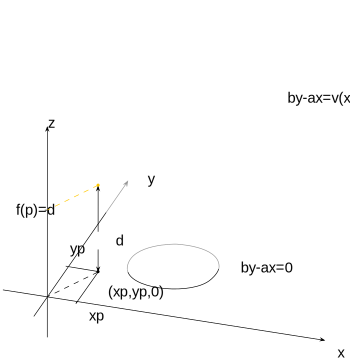
\includegraphics{figures/source/plot11}};


\path[draw=c989898,line join=round,line width=0.512pt] (173.2880,332.6840) -- (173.2970,290.3690);



\path[draw=c989898,line join=round,line width=0.512pt] (173.2970,288.2890) -- (173.3150,213.6110);



\path[draw=c989898,line join=round,line width=0.512pt] (173.3160,211.2310) -- (173.3390,113.4170);



\path[draw=black,line join=round,line width=0.512pt] (47.3201,297.3570) -- (324.8360,340.8940);



\path[draw=black,line join=round,line width=0.512pt] (47.3393,297.7850) -- (47.3804,127.3150);



\path[draw=black,line join=round,line width=0.512pt] (47.3257,337.8570) -- (47.3354,297.7680);



\path[draw=black,line join=round,line width=0.512pt] (47.2678,297.6320) -- (83.2534,245.9200);



\path[draw=black,line join=round,line width=0.512pt] (92.4553,232.6970) -- (105.4110,214.0800);



\path[draw=c989898,line join=round,line width=0.512pt] (107.5070,211.0670) -- (113.9760,201.7710);



\path[draw=c989898,line join=round,line width=0.512pt] (116.0050,198.8560) -- (127.7670,181.9540);



\path[fill=black,line join=round,line width=0.160pt] (45.1337,132.1130) -- (47.4067,130.1080) -- (49.4902,132.1040) -- (47.3042,126.3360) -- (45.1337,132.1130) -- cycle;



\path[fill=black,line join=round,line width=0.160pt] (320.4950,337.6730) -- (322.0070,340.2990) -- (319.6360,341.9440) -- (325.7240,340.9500) -- (320.4950,337.6730) -- cycle;



\path[cm={{1.0,0.0,0.0,1.0,(323.0,358.0)}}] (0.0000,0.0000) node[above right] () {$x$};



\path[cm={{1.0,0.0,0.0,1.0,(33.0,128.0)}}] (0.0000,0.0000) node[above right] () {$z$};



\path[cm={{1.0,0.0,0.0,1.0,(133.0,184.0)}}] (0.0000,0.0000) node[above right] () {$y$};



\path[draw=c989898,fill=c989898,line join=round,line width=0.160pt] (123.4090,184.7720) -- (126.3920,184.2350) -- (127.1390,187.0210) -- (128.2590,180.9550) -- (123.4090,184.7720) -- cycle;



\path[draw=black,line join=round,line width=0.512pt] (33.8411,316.9190) -- (47.2875,297.6020);



\path[draw=c989898,line join=round,line width=0.512pt] (219.3400,268.1300) .. controls (219.4020,267.7220) and (219.4350,267.3120) .. (219.4350,266.9020) .. controls (219.4350,246.0400) and (175.9680,244.5180) .. (175.9680,244.5180);



\path[draw=c989898,line join=round,line width=0.512pt] (170.9090,244.6550) .. controls (159.1350,245.2810) and (130.6670,248.6840) .. (127.5750,266.9020) .. controls (127.3910,267.9820) and (127.3660,269.0270) .. (127.4870,270.0360);



\path[draw=c989898,line join=round,line width=0.512pt] (127.4870,270.0360) .. controls (127.5930,270.9230) and (127.8120,271.7810) .. (128.1350,272.6120);



\path[draw=black,line join=round,line width=0.512pt] (128.1350,272.6120) .. controls (135.2830,291.0080) and (193.4860,295.5780) .. (210.9770,280.0880) .. controls (210.9770,280.0880) and (217.3970,275.0510) .. (219.0510,269.4220);



\path[draw=c989898,line join=round,line width=0.512pt] (219.0510,269.4220) .. controls (219.1760,268.9940) and (219.2750,268.5630) .. (219.3400,268.1300);

%here is the upper circle
\path[draw=black,line join=round,line width=0.512pt] (98.5146,184.9420) .. controls (110.1230,214.8150) and (204.6360,222.2350) .. (233.0370,197.0820) .. controls (233.0370,197.0820) and (243.4630,188.9020) .. (246.1480,179.7620);


\path[fill=foo,line join=round,line width=0.160pt] (84.9343,148.9700) -- (86.9687,145.2070) -- (90.8356,147.3020) -- (85.2988,139.7020) -- (84.9343,148.9700) -- cycle;



\path[draw=c989898,line join=round,line width=0.512pt] (246.1880,179.7470) .. controls (246.2880,179.0870) and (246.3410,178.4250) .. (246.3410,177.7630) .. controls (246.3410,144.0430) and (176.0870,141.5840) .. (176.0870,141.5840) .. controls (176.0870,141.5840) and (175.8910,141.5810) .. (175.5170,141.5810);



\path[draw=c989898,line join=round,line width=0.512pt] (171.7840,141.6430) .. controls (156.1870,142.1140) and (103.2510,146.0570) .. (97.8694,177.7630) .. controls (97.5732,179.5090) and (97.5329,181.1970) .. (97.7282,182.8280);



\path[fill=foo,line join=round,line width=0.160pt] (98.2177,183.9090) .. controls (99.0719,183.9090) and (99.7643,184.6020) .. (99.7643,185.4560) .. controls (99.7643,186.3100) and (99.0719,187.0030) .. (98.2177,187.0030) .. controls (97.3635,187.0030) and (96.6710,186.3100) .. (96.6710,185.4560) .. controls (96.6710,184.6020) and (97.3635,183.9090) .. (98.2177,183.9090) -- cycle;



\path[draw=black,line join=round,line width=0.512pt] (44.8080,210.4840) -- (47.5576,210.4910);



\path[cm={{1.0,0.0,0.0,1.0,(-10.0,215.0)}}] (0.0000,0.0000) node[above right] () {$\varphi(\mathbf{p})=d_2$};



\path[fill=foo,line join=round,line width=0.256pt] (88.6971,190.5360) -- (83.9057,192.8790) -- (83.6246,192.3040) -- (88.4160,189.9610) -- (88.6971,190.5360) -- cycle(79.1143,195.2210) -- (74.3230,197.5640) -- (74.0419,196.9890) -- (78.8333,194.6460) -- (79.1143,195.2210) -- cycle(69.5316,199.9060) -- (64.7402,202.2490) -- (64.4592,201.6740) -- (69.2505,199.3310) -- (69.5316,199.9060) -- cycle(59.9489,204.5910) -- (55.1575,206.9340) -- (54.8764,206.3590) -- (59.6678,204.0160) -- (59.9489,204.5910) -- cycle(50.3661,209.2760) -- (47.4761,210.6890) -- (47.1950,210.1140) -- (50.0851,208.7010) -- (50.3661,209.2760) -- cycle(98.2798,185.8510) -- (93.4884,188.1940) -- (93.2073,187.6190) -- (97.9987,185.2760) -- (98.2798,185.8510) -- cycle;



\path[cm={{1.0,0.0,0.0,1.0,(209.0,252.0)}}] (0.0000,0.0000) node[above right] () {$(x-3)^2+(y-3)^2-2=h$};



\path[draw=foo,fill=foo,line join=round,line width=0.160pt] (111.5160,222.6330) -- (109.6890,226.5640) -- (105.7670,224.5760) -- (111.5090,232.0200) -- (111.5160,222.6330) -- cycle;



\path[draw=foo,line join=round,line width=1.080pt] (98.2124,185.3970) -- (109.6740,227.0900);



\path[fill=foo,line join=round,line width=0.160pt] (173.2540,332.7580) .. controls (174.1080,332.7580) and (174.8000,333.4510) .. (174.8000,334.3050) .. controls (174.8000,335.1590) and (174.1080,335.8520) .. (173.2540,335.8520) .. controls (172.4000,335.8520) and (171.7070,335.1590) .. (171.7070,334.3050) .. controls (171.7070,333.4510) and (172.4000,332.7580) .. (173.2540,332.7580) -- cycle;



\path[cm={{1.0,0.0,0.0,1.0,(59.0,151.0)}}] (0.0000,0.0000) node[above right] () {$\nabla\varphi_i$};



\path[cm={{1.0,0.0,0.0,1.0,(78.0,247.0)}}] (0.0000,0.0000) node[above right] () {$-\nabla\varphi_i$};



\path[cm={{1.0,0.0,0.0,1.0,(161.0,351.0)}}] (0.0000,0.0000) node[above right] () {$\nabla\varphi_i=0$};



\path[fill=c989898,line join=round,line width=0.160pt] (173.3130,266.0410) .. controls (174.1670,266.0410) and (174.8590,266.7340) .. (174.8590,267.5880) .. controls (174.8590,268.4420) and (174.1670,269.1340) .. (173.3130,269.1340) .. controls (172.4580,269.1340) and (171.7660,268.4420) .. (171.7660,267.5880) .. controls (171.7660,266.7340) and (172.4580,266.0410) .. (173.3130,266.0410) -- cycle;



\path[fill=c989898,line join=round,line width=0.160pt] (173.2130,176.3380) .. controls (174.0670,176.3380) and (174.7590,177.0300) .. (174.7590,177.8840) .. controls (174.7590,178.7390) and (174.0670,179.4310) .. (173.2130,179.4310) .. controls (172.3590,179.4310) and (171.6660,178.7390) .. (171.6660,177.8840) .. controls (171.6660,177.0300) and (172.3590,176.3380) .. (173.2130,176.3380) -- cycle;



\path[draw=foo,line join=round,line width=1.080pt] (86.8208,143.8110) -- (98.2827,185.5040);




\end{tikzpicture}


  \caption[.]{.}
  \label{fig:grad}
\end{figure}
Immagine for an instant that our goal is not to fly over the circle in \fref{fig:plot11}{Figure}, but to its center $(x_c,y_c)$ in \frefeq{eq:pathf-circle}. The vector field $\varPhi$ in \frefeq{eq:vec-field-def} direct us in the opposite direction; we can then use $-\nabla\varphi_i$ to direct to robot to the goal.

Vector fields are common used in the motion planning literature for navigation of different mobile robots~\citep{lindemann2005smoothly,gonccalves2010vector,panagou2014motion,zhou2014vector,kapitanyuk2017guiding,de2017guidance}, and are also threated in some robots planning textbooks~\citep{choset2005principles,lavalle2006planning}. A well-known intuitive method brought from optimization is the gradient descent algorithm\findex{gradient descent algorithm}~\citep{choset2005principles,bryson1975applied}, where an intuitive choice of the search direction is the negative gradient $\Delta \varphi_i:=-\nabla\varphi_i$~\citep{boyd2004convex}. We illustrate the gradient descent algorithm in \fref{algo:grad-desc}{Algorithm} where we iterate at discrete time steps (i.e., at instant $n$, $\mathcal{K}$ contains $t_0,t_0+h,\dots,t_0+nh$; we discuss further the time step $h$ ($h$ is not to be confused with the altitude when used in the path functions) later in this chapter in \fref{sec:algo}{Section}), $\mathbf{p}(t_0)$ is given (e.g., from sensors data), $\theta(i)$ is a scalar step size at time instant $i$~\citep{choset2005principles}--there can be indeed different step sizes at different instants--and $\varepsilon\in\mathbb{R}_{>0}$ is chosen based on the task requirements (it is unrealistic to assume we will reach $\nabla\varphi_i=0$).

\begin{algorithm}[h!] %this is an example
  \SetKwInOut{Input}{Input}
  \SetKwInOut{Output}{Output}
  \SetKwFunction{FMain}{\small\tt zamboni-like\_motion}
  \SetKwProg{Fn}{Function}{:}{}
  \SetKwProg{Pn}{Function}{:}{\KwRet}

  \DontPrintSemicolon
  \Input{$t_0${ \otherfont initial time step}\newline
         $c^\rho_i${ \otherfont value of the path parameters}\newline
         $j${ \otherfont current stage}
  }
  \Output{$\mathbf{p}(\mathcal{K})${ \otherfont trajectory}
  }
  \vspace{.8ex}

  \ForEach{\normalsize $i\in\mathcal{K}:=\{t_0,t_0+h,t_0+2h,\dots\}$}{
    \If{\normalsize $\norm{\nabla\varphi_j(\mathbf{p}(t),c^\rho_i)}\leq \varepsilon$}{
      \vspace{.8ex}
      \Return{\normalsize $\mathbf{p}(\mathcal{K})$}\;
    }
    {\normalsize $\mathbf{p}(i+h)\gets \mathbf{p}(i)+\theta(i)\Delta\varphi_j(\mathbf{p}(t),c^\rho_i)$}\;
  }
  \vspace{.8ex}

  \caption{Gradient descent}\findex{gradient descent}
  \label{algo:grad-desc}
\end{algorithm}

\fref{algo:grad-desc}{Algorithm} that we illustrate in \fref{fig:grad_desc}{Figure} directs us to the center of the circle in case we have a circle as a path function.
\begin{figure}[h!]
  \centering
  \fontfamily{phv}\selectfont
  
\definecolor{c989898}{RGB}{152,152,152}
\small

\def \globalscale {1.000000}
\begin{tikzpicture}[y=0.80pt, x=0.80pt, yscale=-\globalscale, xscale=\globalscale, inner sep=0pt, outer sep=0pt]
\path[draw=black,line join=round,line width=0.512pt] (10.4871,206.0790) -- (222.2210,206.0800);



\path[draw=black,line join=round,line width=0.512pt] (16.1042,10.3269) -- (16.1041,128.8180);



\path[draw=black,line join=round,line width=0.512pt] (16.1041,148.0200) -- (16.1041,212.0610);



\path[fill=black,line join=round,line width=0.160pt] (14.1422,14.1208) -- (16.1124,12.3829) -- (17.9183,14.1129) -- (16.0235,9.1129) -- (14.1422,14.1208) -- cycle;



\path[fill=black,line join=round,line width=0.160pt] (220.0700,204.0730) -- (221.8080,206.0430) -- (220.0780,207.8490) -- (225.0780,205.9540) -- (220.0700,204.0730) -- cycle;



\path[draw=c989898,line join=round,line width=0.512pt] (149.8410,78.8284) .. controls (154.3410,84.7637) and (157.0120,92.1629) .. (157.0120,100.1860) .. controls (157.0120,119.7270) and (141.1700,135.5680) .. (121.6290,135.5680) .. controls (102.0880,135.5680) and (86.2470,119.7270) .. (86.2470,100.1860) .. controls (86.2470,80.6446) and (102.0880,64.8033) .. (121.6290,64.8033) .. controls (129.8280,64.8033) and (137.3750,67.5916) .. (143.3740,72.2717);



\path[draw=c989898,line join=round,line width=0.512pt] (182.5090,96.6832) .. controls (182.5660,97.7650) and (182.5950,98.8543) .. (182.5950,99.9503) .. controls (182.5950,133.6210) and (155.2990,160.9160) .. (121.6290,160.9160) .. controls (87.9590,160.9160) and (60.6638,133.6210) .. (60.6638,99.9503) .. controls (60.6638,66.2801) and (87.9590,38.9848) .. (121.6290,38.9848) .. controls (150.9150,38.9848) and (175.3790,59.6349) .. (181.2530,87.1686);



\path[draw=c989898,line join=round,line width=0.512pt] (145.1750,24.6380) .. controls (177.2720,34.6552) and (200.5690,64.6102) .. (200.5690,100.0060) .. controls (200.5690,143.6030) and (165.2260,178.9460) .. (121.6290,178.9460) .. controls (78.0322,178.9460) and (42.6898,143.6030) .. (42.6898,100.0060) .. controls (42.6898,56.4095) and (78.0322,21.0669) .. (121.6290,21.0669) .. controls (125.2030,21.0669) and (128.7210,21.3043) .. (132.1690,21.7643);



\path[draw=black,line join=round,line width=0.512pt] (169.1290,84.0395) .. controls (170.8430,89.0955) and (171.7730,94.5140) .. (171.7730,100.1490) .. controls (171.7730,127.8430) and (149.3230,150.2930) .. (121.6290,150.2930) .. controls (93.9356,150.2930) and (71.4855,127.8430) .. (71.4855,100.1490) .. controls (71.4855,72.4559) and (93.9356,50.0056) .. (121.6290,50.0056) .. controls (140.6690,50.0056) and (157.2300,60.6169) .. (165.7210,76.2480);



\path[draw=c989898,line join=round,line width=0.512pt] (123.3230,13.4268) .. controls (170.3700,14.3427) and (208.2270,52.7672) .. (208.2270,100.0330) .. controls (208.2270,147.8740) and (169.4450,186.6560) .. (121.6040,186.6560) .. controls (73.7637,186.6560) and (34.9813,147.8740) .. (34.9813,100.0330) .. controls (34.9813,56.4761) and (67.1302,20.4270) .. (108.9940,14.3212);



\path[draw=c989898,line join=round,line width=0.512pt] (158.4340,39.8940) .. controls (178.6100,52.2827) and (192.0660,74.5505) .. (192.0660,99.9615) .. controls (192.0660,138.8630) and (160.5300,170.3980) .. (121.6290,170.3980) .. controls (82.7282,170.3980) and (51.1927,138.8630) .. (51.1927,99.9615) .. controls (51.1927,61.0606) and (82.7282,29.5249) .. (121.6290,29.5249) .. controls (130.9120,29.5249) and (139.7750,31.3205) .. (147.8900,34.5835);



\path[fill=foo,line join=round,line width=0.160pt] (121.4980,98.8207) .. controls (122.2380,98.8207) and (122.8380,99.4209) .. (122.8380,100.1610) .. controls (122.8380,100.9020) and (122.2380,101.5020) .. (121.4980,101.5020) .. controls (120.7570,101.5020) and (120.1570,100.9020) .. (120.1570,100.1610) .. controls (120.1570,99.4209) and (120.7570,98.8207) .. (121.4980,98.8207) -- cycle;



\path[fill=foo,line join=round,line width=0.160pt] (50.9590,135.0120) ellipse (0.0378cm and 0.0378cm);



\path[draw=foo,line join=round,line width=0.512pt] (51.0193,135.0320) -- (58.2991,131.4430);



\path[fill=foo,line join=round,line width=0.256pt] (63.0120,128.9410) -- (65.4039,127.7620) -- (65.5453,128.0490) -- (63.1535,129.2280) -- (63.0120,128.9410) -- cycle(67.7957,126.5830) -- (70.1875,125.4040) -- (70.3290,125.6910) -- (67.9372,126.8700) -- (67.7957,126.5830) -- cycle(72.5794,124.2250) -- (74.9712,123.0460) -- (75.1127,123.3330) -- (72.7209,124.5120) -- (72.5794,124.2250) -- cycle(77.3631,121.8670) -- (79.7549,120.6880) -- (79.8964,120.9750) -- (77.5045,122.1540) -- (77.3631,121.8670) -- cycle(82.1467,119.5090) -- (84.5386,118.3300) -- (84.6801,118.6170) -- (82.2882,119.7960) -- (82.1467,119.5090) -- cycle(86.9304,117.1510) -- (89.3222,115.9720) -- (89.4637,116.2590) -- (87.0719,117.4380) -- (86.9304,117.1510) -- cycle(91.7141,114.7930) -- (94.1059,113.6130) -- (94.2474,113.9010) -- (91.8556,115.0800) -- (91.7141,114.7930) -- cycle(96.4978,112.4340) -- (98.8896,111.2550) -- (99.0311,111.5420) -- (96.6393,112.7210) -- (96.4978,112.4340) -- cycle(101.2810,110.0760) -- (103.6730,108.8970) -- (103.8150,109.1840) -- (101.4230,110.3630) -- (101.2810,110.0760) -- cycle(106.0650,107.7180) -- (108.4570,106.5390) -- (108.5980,106.8260) -- (106.2070,108.0050) -- (106.0650,107.7180) -- cycle(110.8490,105.3600) -- (113.2410,104.1810) -- (113.3820,104.4680) -- (110.9900,105.6470) -- (110.8490,105.3600) -- cycle(115.6320,103.0020) -- (118.0240,101.8230) -- (118.1660,102.1100) -- (115.7740,103.2890) -- (115.6320,103.0020) -- cycle(120.4160,100.6440) -- (121.6180,100.0510) -- (121.7600,100.3380) -- (120.5580,100.9310) -- (120.4160,100.6440) -- cycle(58.2284,131.3000) -- (60.6202,130.1210) -- (60.7617,130.4080) -- (58.3698,131.5870) -- (58.2284,131.3000) -- cycle;



\path[fill=foo,line join=round,line width=0.160pt] (58.4502,131.3860) ellipse (0.0378cm and 0.0378cm);



\path[fill=foo,line join=round,line width=0.160pt] (66.9795,125.6080) .. controls (67.7198,125.6080) and (68.3201,126.2080) .. (68.3201,126.9480) .. controls (68.3201,127.6890) and (67.7198,128.2890) .. (66.9795,128.2890) .. controls (66.2390,128.2890) and (65.6388,127.6890) .. (65.6388,126.9480) .. controls (65.6388,126.2080) and (66.2390,125.6080) .. (66.9795,125.6080) -- cycle;



\path[fill=foo,line join=round,line width=0.160pt] (76.6875,120.9270) .. controls (77.4279,120.9270) and (78.0281,121.5270) .. (78.0281,122.2680) .. controls (78.0281,123.0080) and (77.4279,123.6080) .. (76.6875,123.6080) .. controls (75.9471,123.6080) and (75.3468,123.0080) .. (75.3468,122.2680) .. controls (75.3468,121.5270) and (75.9471,120.9270) .. (76.6875,120.9270) -- cycle;



\path[fill=foo,line join=round,line width=0.160pt] (89.7933,114.2820) .. controls (90.5337,114.2820) and (91.1339,114.8820) .. (91.1339,115.6220) .. controls (91.1339,116.3630) and (90.5337,116.9630) .. (89.7933,116.9630) .. controls (89.0529,116.9630) and (88.4527,116.3630) .. (88.4527,115.6220) .. controls (88.4527,114.8820) and (89.0529,114.2820) .. (89.7933,114.2820) -- cycle;



\path[cm={{1.0,0.0,0.0,1.0,(166.0,82.0)}}] (0.0000,0.0000) node[above right] () {\footnotesize $h$};



\path[cm={{1.0,0.0,0.0,1.0,(141.0,78.0)}}] (0.0000,0.0000) node[above right] () {\scriptsize -1};



\path[cm={{1.0,0.0,0.0,1.0,(175.0,95.0)}}] (0.0000,0.0000) node[above right] () {\scriptsize +1};



\path[cm={{1.0,0.0,0.0,1.0,(146.0,41.0)}}] (0.0000,0.0000) node[above right] () {\scriptsize +2};



\path[cm={{1.0,0.0,0.0,1.0,(133.0,27.0)}}] (0.0000,0.0000) node[above right] () {\scriptsize +3};



\path[cm={{1.0,0.0,0.0,1.0,(110.0,16.0)}}] (0.0000,0.0000) node[above right] () {\scriptsize +4};



\path[cm={{1.0,0.0,0.0,1.0,(222.0,222.0)}}] (0.0000,0.0000) node[above right] () {$x$};



\path[cm={{1.0,0.0,0.0,1.0,(0.0,7.0)}}] (0.0000,0.0000) node[above right] () {$y$};



\path[cm={{1.0,0.0,0.0,1.0,(110.0,119.0)}}] (0.0000,0.0000) node[above right] () {$\nabla\varphi_i=0$};



\path[cm={{1.0,0.0,0.0,1.0,(42.0,196.0)}}] (0.0000,0.0000) node[above right] () {$\mathbf{p}(t_0+h)$};



\path[draw=black,line join=round,line width=0.512pt] (51.6569,181.8440) .. controls (51.6569,181.8440) and (43.5503,166.9640) .. (48.7769,158.0040) .. controls (54.0036,149.0440) and (57.4702,146.6280) .. (58.6435,135.1080);



\path[cm={{1.0,0.0,0.0,1.0,(1.0,143.5)}}] (0.0000,0.0000) node[above right] () {$\mathbf{p}(t_0)$};



\path[draw=black,line join=round,line width=0.512pt] (24.5102,135.5880) .. controls (24.5102,135.5880) and (27.5769,136.2540) .. (35.3635,134.2280) .. controls (40.6100,132.8620) and (41.7368,130.6280) .. (47.3369,133.0810);




\end{tikzpicture}


  \caption[.]{.}
  \label{fig:grad_desc}
\end{figure}
However, we are interested into following these paths at an assigned altitude, i.e., we want to track the functions in \frefeq{eq:two-paths}. Concretely, in the path sub-plan that we proposed in \frefeqM{eq:line-gene}{eq:circ-gene} in \fref{sec:path-wise}{Section}, we want to track, e.g., the path function $\varphi_{i+1}$ by flying over the function rather that heading the center of the circle it describes; we started tracking the function after reaching $\mathbf{p}_{\Gamma_i}$ while tracking $\varphi_i$ and so on. To this end, we use a vector field-based approach proposed in the literature specifically for aerial robots~\citep{de2017guidance}, which points to the contours of the functions in \fref{fig:plot1}{Figures}\fref{fig:plot11}{--\hspace{-.8ex}} and thus to \frefeq{eq:two-paths}.

The expression for the search direction $\Delta\varphi_i$ in~\citep{de2017guidance} becomes
\begin{equation}\label{eq:pd}
  \Delta_d\varphi_i(\mathbf{p}(t),c_i^\rho):=E_i\nabla\varphi_i(\mathbf{p}(t),c_i^\rho)-k_e\varphi_i(\mathbf{p}(t),c_i^\rho)\nabla\varphi_i(\mathbf{p}(t),c_i^\rho),
\end{equation}
where $E_i\nabla\varphi_i(\mathbf{p}(t),c_i^\rho)$ is a vector pointing perpendicularly to the gradient $\nabla\varphi_i(\mathbf{p}(t),c_i^\rho)$, $E_i$ is the $i$th stage direction
\begin{equation}
  E_i=\begin{bmatrix}
    0&1\\-1&0
  \end{bmatrix},
\end{equation}
with $E_i$ being the counter clockwise, $-E_i$ the clockwise direction. 
The contribution of the component $-k_e\varphi_i(\mathbf{p}(t),c_i^\rho)\nabla\varphi_i(\mathbf{p}(t),c_i^\rho)$ in \frefeq{eq:pd} points then in the direction of the path function. It depends on the coefficient $k_e\in\mathbb{R}_{>0}$--indicating the speed of convergence~\citep{de2017guidance}--and on the value of $\varphi_i$ at the current point (of course also on the path parameters and the value of the gradient). We illustrate $\Delta_d\varphi_i$ in \fref{}{Figure}. When we take a point within the circle, let's call it $\mathbf{p}_{-}$, the value of $\varphi_i$ is negative; $-k_e\varphi_i(\mathbf{p}_{-},c_i^\rho)\nabla\varphi_i(\mathbf{p}_{-},c_i^\rho)$ points outwards of the circle center, in the direction of the path function. $E_i\nabla\varphi_i(\mathbf{p}_{-},c_i^\rho)$ points perpendicularly to the gradient $\nabla\varphi_i$ and to the path function itself. The resulting vector $\Delta_d\varphi_i(\mathbf{p}_{-},c_i^\rho)$ then points the direction of the path function.

Now we take a point $\mathbf{p}_{+}$ out of the circle, and not exactly over the path function. The value of $\varphi_i$ is positive; $-k_e\varphi_i(\mathbf{p}_{+},c_i^\rho)\nabla\varphi_i(\mathbf{p}_{+},c_i^\rho)$ points inwards of the circle center and the resulting vector $\Delta_d\varphi_i(\mathbf{p}_{-},c_i^\rho)$ in the direction of the path function. If we finally take a point $\mathbf{p}_{0}$ exactly over the path function, $\varphi_i$ is zero; $-k_e\varphi_i(\mathbf{p}_{0},c_i^\rho)\nabla\varphi_i(\mathbf{p}_{0},c_i^\rho)$ is thus also zero and $\Delta_d\varphi_i(\mathbf{p}_{0},c_i^\rho)$ points perpendicularly to the path functions. Let us thus define the vector fields
\begin{equation}
  \varPhi_d(t,\varphi_i,c_i^\rho):=\bigcup\limits_{\mathbf{p}(t)\in\mathcal{Q}^v}{\Delta_d\varphi_i{\mathbf{p}(t),c_i^\rho}}.
\end{equation}

This vector fields points to the path function such as the line and the circle in \frefeq{eq:two-paths} for every point in space $\mathcal{Q}^v$ as we illustrate in \fref{}{Figure} for the line $2y-x=h$ and in \fref{}{Figure} for the circle $(x-3)^2+(y-3)^2-2=h$.

\begin{algorithm}[h!] %this is an example
  \SetKwInOut{Input}{Input}
  \SetKwInOut{Output}{Output}
  \SetKwFunction{FMain}{\small\tt zamboni-like\_motion}
  \SetKwProg{Fn}{Function}{:}{}
  \SetKwProg{Pn}{Function}{:}{\KwRet}

  \DontPrintSemicolon
  \Input{$t_0${ \otherfont initial time step}\newline
         $c^\rho_i${ \otherfont value of the path parameters}\newline
         $j${ \otherfont current stage}
  }
  \Output{$\mathbf{p}(\mathcal{K})${ \otherfont trajectory}
  }
  \vspace{.8ex}

  \ForEach{\normalsize $i\in\mathcal{K}:=\{t_0,t_0+h,t_0+2h,\dots\}$}{\label{algo:track:foreach}
    \If{\normalsize $\norm{\mathbf{p}(i)-\mathbf{p}_{\Gamma_j}}\leq \varepsilon$}{\label{algo:track:eucly}
      \vspace{.8ex}
      \Return{\normalsize $\mathbf{p}(\mathcal{K})$}\;
    }
    {\normalsize $\mathbf{p}(i+h)\gets \mathbf{p}(i)+\theta(i)\Delta_d\varphi_j(\mathbf{p}(i),c_j^\rho)$}\;\label{algo:track:gvf}
  }
  \vspace{.8ex}

  \caption{Path function tracking}\findex{tracking}
  \label{algo:track}
\end{algorithm}


Finally, let's reconsider \fref{algo:grad-desc}{Algorith} with the vector field $\varPhi_d$ and guide the aerial robot in space to track a specific path function $\varphi_i$ in \fref{algo:track}{Algorithm}. The algorithm iterates at discrete time steps on \fref{algo:track:foreach}{Line} as \fref{algo:grad-desc}{Algorith}. It stops tracking the $j$th path function at occurrence of the triggering point $\mathbf{p}_{\Gamma_j}$ on \fref{algo:track:eucly}{Line} using the Euclidean distance with a small enough $\varepsilon\in\mathbb{R}_{>0}$ rather than evaluating if the function reached a local minimum with $\nabla\varphi_j=0$ in \fref{algo:grad-desc}{Algorithm}. The algorithm then computes a simplified version of the next position  on \fref{algo:track:gvf}{Line} using the current position $\mathbf{p}(i)$ and the gradient $\Delta_d\varphi_i$ without considering vehicles' velocity $v(i)$ and other parameters (such as external interferences, e.g., wind speed and direction). For simplicity, we can use the same value for the time step $h$ that we used for the step size $\theta$ for all the time instants in $\mathcal{K}$.



\subsection{\color{red}Derivation of the guidance action}


%%%%%%%%%%%%%%%%%%%%%%%%%%%%%%%%
\section{Coverage Path Planning}
\label{sec:cov-path-plan}\findex{coverage path planning}

In this section, we solve \fref{pb:cov-pb}{Problem}. Let us recall briefly our objective of providing a set of paths (a tour) in the plan from \fref{def:plan}{Definition} to cover each point in a given space. We summarize such space with a set of vertices $v:=\{v_1,v_2,\dots\}$ that form a polygon. The robot is free to move within the polygon except for some obstacles described by other sets of vertices, one per each obstacle $o_1:=\{o_{1,1},o_{1,2},\dots\},o_2:=\{o_{2,1},o_{2,2},\dots\},\dots$. There are several different approaches in the literature to solve this problem. We have detailed the approaches in the literature in \fref{sec:soa-cov-path-plan}{Sections}\fref{sec:opti-cov}{--\hspace{-.8ex}} for mobile robots and in \fref{sec:cov-plan-aero}{Sections}\fref{sec:opti-aero-cov}{--\hspace{-.8ex}} for aerial robots specifically. In summary, the sub-class of motion planning that finds the coverage tour of a given space is called coverage path planning (CPP)~\citep{choset1998coverage}. The algorithms for the coverage tour are NP-hard\findex{NP-hard}~\citep{arkin2000approximation} and use either implicitly or explicitly the cellular decomposition that divides the robot's free space into sub-regions that can be easily covered~\citep{choset2001coverage,galceran2013survey}.

There are numerous methodologies for cellular decomposition itself. Some decompose the polygon into equally sized sub-regions that form a grid and then visits only the sub-regions where the robot is free to move~\citep{galceran2013survey}. 
\begin{figure}[h!]
  \centering
  \fontfamily{phv}\selectfont
  
\definecolor{cD9D9D9}{RGB}{217,217,217}
\footnotesize
\def \globalscale {1.000000}
\begin{tikzpicture}[y=0.80pt, x=0.80pt, yscale=-\globalscale, xscale=\globalscale, inner sep=0pt, outer sep=0pt]
\path[draw=black,line join=round,line width=0.512pt] (18.6584,24.2061) -- (183.9870,7.5586) -- (183.9870,107.9380) -- (18.6584,124.5850) -- (18.6584,24.2061) -- cycle;



\path[draw=black,fill=cD9D9D9,line join=round,line width=0.256pt] (67.8359,72.3465) -- (79.1010,53.2824) -- (102.1880,45.5971) -- (127.8940,56.4066) -- (124.7750,79.5434) -- (80.3210,91.5016) -- (67.8359,72.3465) -- cycle;



\path[cm={{1.0,0.0,0.0,1.0,(0.0,27.0)}}] (0.0000,0.0000) node[above right] () {$v_1$};

\path[cm={{1.0,0.0,0.0,1.0,(0.0,126.0)}}] (0.0000,0.0000) node[above right] () {$v_4$};

\path[cm={{1.0,0.0,0.0,1.0,(190.0,7.0)}}] (0.0000,0.0000) node[above right] () {$v_2$};

\path[cm={{1.0,0.0,0.0,1.0,(190.0,109.0)}}] (0.0000,0.0000) node[above right] () {$v_3$};

\path[cm={{1.0,0.0,0.0,1.0,(52.0,69.0)}}] (0.0000,0.0000) node[above right] () {$o_{1,1}$};

\path[cm={{1.0,0.0,0.0,1.0,(63.0,52.0)}}] (0.0000,0.0000) node[above right] () {$o_{1,2}$};

\path[cm={{1.0,0.0,0.0,1.0,(94.0,45.0)}}] (0.0000,0.0000) node[above right] () {$o_{1,3}$};

\path[cm={{1.0,0.0,0.0,1.0,(135.0,60.0)}}] (0.0000,0.0000) node[above right] () {$o_{1,4}$};

\path[cm={{1.0,0.0,0.0,1.0,(127.0,88.0)}}] (0.0000,0.0000) node[above right] () {$o_{1,5}$};

\path[cm={{1.0,0.0,0.0,1.0,(66.0,100.0)}}] (0.0000,0.0000) node[above right] () {$o_{1,6}$};



\path[draw=black,line join=round,line width=0.256pt] (18.6285,54.5004) -- (134.7670,54.5001);



\path[draw=black,line join=round,line width=0.256pt] (155.5270,54.5004) -- (184.0610,54.5001);



\path[draw=black,line join=round,line width=0.256pt] (18.6285,24.5004) -- (184.0610,24.5001);



\path[draw=black,line join=round,line width=0.256pt] (18.6285,34.5004) -- (184.0610,34.5001);



\path[draw=black,line join=round,line width=0.256pt] (18.6285,44.5004) -- (62.1670,44.5003);



\path[draw=black,line join=round,line width=0.256pt] (81.7806,44.5003) -- (93.4071,44.5003);



\path[draw=black,line join=round,line width=0.256pt] (113.9670,44.5006) -- (184.0610,44.5001);



\path[draw=black,line join=round,line width=0.256pt] (18.6285,94.5004) -- (63.9474,94.5003);



\path[draw=black,line join=round,line width=0.256pt] (83.6273,94.5002) -- (184.0610,94.5001);



\path[draw=black,line join=round,line width=0.256pt] (18.6285,84.5004) -- (126.4200,84.5001);



\path[draw=black,line join=round,line width=0.256pt] (144.7140,84.5001) -- (184.0610,84.5001);



\path[draw=black,line join=round,line width=0.256pt] (18.6285,74.5004) -- (184.0610,74.5001);



\path[draw=black,line join=round,line width=0.256pt] (18.6285,64.5004) -- (50.5273,64.5003);



\path[draw=black,line join=round,line width=0.256pt] (69.6273,64.5003) -- (184.0610,64.5001);



\path[draw=black,line join=round,line width=0.256pt] (18.6285,104.5000) -- (184.0610,104.5000);



\path[draw=black,line join=round,line width=0.256pt] (18.6285,114.5000) -- (119.0600,114.5050);



\path[draw=black,line join=round,line width=0.256pt] (115.6280,14.5024) -- (184.0610,14.5001);



\path[draw=black,line join=round,line width=0.256pt] (118.6220,14.1766) -- (118.6250,114.6100);



\path[draw=black,line join=round,line width=0.256pt] (108.6230,15.1767) -- (108.6230,36.0018);



\path[draw=black,line join=round,line width=0.256pt] (108.6240,45.2420) -- (108.6260,115.6100);



\path[draw=black,line join=round,line width=0.256pt] (98.6223,16.1766) -- (98.6230,36.0302);



\path[draw=black,line join=round,line width=0.256pt] (98.6241,45.3706) -- (98.6257,116.6100);



\path[draw=black,line join=round,line width=0.256pt] (88.6223,17.1766) -- (88.6258,117.6100);



\path[draw=black,line join=round,line width=0.256pt] (78.6222,18.1766) -- (78.6228,42.2150);



\path[draw=black,line join=round,line width=0.256pt] (78.6234,52.4953) -- (78.6248,90.0419);



\path[draw=black,line join=round,line width=0.256pt] (78.6251,99.8153) -- (78.6258,118.6100);



\path[draw=black,line join=round,line width=0.256pt] (68.6223,19.1766) -- (68.6236,42.1817);



\path[draw=black,line join=round,line width=0.256pt] (68.6244,52.2773) -- (68.6245,59.1362);



\path[draw=black,line join=round,line width=0.256pt] (68.6249,68.8953) -- (68.6254,90.3623);



\path[draw=black,line join=round,line width=0.256pt] (68.6258,99.7889) -- (68.6263,119.6100);



\path[draw=black,line join=round,line width=0.256pt] (58.6232,20.1764) -- (58.6241,59.2753);



\path[draw=black,line join=round,line width=0.256pt] (58.6244,69.0756) -- (58.6263,120.6100);



\path[draw=black,line join=round,line width=0.256pt] (48.6232,21.1765) -- (48.6263,121.6100);



\path[draw=black,line join=round,line width=0.256pt] (28.6232,23.1764) -- (28.6263,123.6100);



\path[draw=black,line join=round,line width=0.256pt] (38.6232,22.1764) -- (38.6263,122.6100);



\path[draw=black,line join=round,line width=0.256pt] (128.6230,13.1767) -- (128.6240,78.0236);



\path[draw=black,line join=round,line width=0.256pt] (128.6250,88.7706) -- (128.6250,113.6100);



\path[draw=black,line join=round,line width=0.256pt] (138.6260,12.1767) -- (138.6260,49.4502);



\path[draw=black,line join=round,line width=0.256pt] (138.6270,60.3504) -- (138.6260,78.0353);



\path[draw=black,line join=round,line width=0.256pt] (138.6260,88.9086) -- (138.6250,112.6100);



\path[draw=black,line join=round,line width=0.256pt] (148.6270,11.1767) -- (148.6260,49.4287);



\path[draw=black,line join=round,line width=0.256pt] (148.6260,60.3688) -- (148.6250,111.5100);



\path[draw=black,line join=round,line width=0.256pt] (158.5930,10.1848) -- (158.5910,110.6180);



\path[draw=black,line join=round,line width=0.256pt] (168.6000,9.1981) -- (168.5980,109.6310);



\path[draw=black,line join=round,line width=0.256pt] (178.5500,8.1813) -- (178.5480,108.6140);




\end{tikzpicture}


  \caption[Grid decomposition]{A polygonal space where we want to find a coverage tour and visit all the points delimited by $v:=\{v_1,\dots,v_4\}$ except for the obstacle $o_1:=\{o_{1,1},\dots,o_{1,6}\}$. A way to cover the space is the grid decomposition that divides the polygon into equally sized cells and visits each cell except the obstacle.}
  \label{fig:gride}
\end{figure}
This methodology is termed grid decomposition\findex{grid decomposition} in~\fref{fig:gride}{Figure}. Another way is to sweep the polygon and divide it into sub-regions\findex{sub-regions} when the sweep line\findex{sweep line} encounters a change in connectivity. We implement this latter class in \fref{sec:cell-deco}{Section}.
Once the algorithm divides the free space into sub-region, it builds an adjacency graph\findex{adjacency graph}. The vertices contain the sub-regions and edges connect adjacent sub-regions~\citep{choset2005principles}. A covering order between the sub-region to derive the sequence of the coverage is then an exhaustive walkthrough of the adjacency graph with, e.g., depth-first search\findex{depth-first search} algorithm~\citep{choset2005principles}. Once divided the space and the order of the coverage, we need to cover each sub-region. We recall that a method is the boustrophedon motion that we discussed in \fref{cp:soa}{Chapter}. However, a generic nonholonomic mobile robot, such as the Opterra fixed-wing craft in the precision agriculture scenario in \fref{sec:motivation}{Section}, has limited maneuverability~\citep{mannadiar2010optimal,xu2011optimal,xu2014efficient}. For a generic aerial robot, it is preferred to have a large turning radius~\citep{wang2017curvature}; to this end, we propose a Zamboni-like motion. We introduced both the Zamboni- and boustrophedon-like motions in \fref{sec:path-wise}{Section}, whereas we implement them later in this chapter in \fref{sec:cov-motion}{Section}.

\subsection{Cellular decomposition of the space}
\label{sec:cell-deco}\findex{cellular decomposition}

In detail, a cellular decomposition decomposes the coverage space into non-overlapping sub-regions called cell\findex{cells}s. Let us define the robot's free space\findex{free space} or the coverage space\findex{coverage space} as $\mathcal{Q}^v$ for an inertial navigation frame $\mathcal{O}_W$. Physically, the free space is where the robot is free to move without intersecting an obstacle~\citep{choset2005principles}. Let $\mathcal{Q}^{o_i}\subset\mathbb{R}^2$ be the space delimited by the obstacle $o_i$. $\mathcal{Q}^v\subseteq\mathbb{R}^2$ contains all the points delimited by the vertices of the polygon $v$ except for $i$ obstacles delimited by the vertices of $i$ polygons $o_i$. The entire space in the polygon $v$, including all the obstacles $o_i$, is then $\mathcal{Q}:=(\bigcup_{i\in|o|}\mathcal{Q}^{o_i})\cup\mathcal{Q}^v$. 
\begin{figure}[h]
  \centering
  \fontfamily{phv}\selectfont
  
\definecolor{cD9D9D9}{RGB}{217,217,217}
\small

\def \globalscale {1.100000}
\begin{tikzpicture}[y=0.80pt, x=0.80pt, yscale=-\globalscale, xscale=\globalscale, inner sep=0pt, outer sep=0pt]
\path[draw=black,line join=round,line width=0.512pt] (18.6584,29.4064) -- (183.9870,12.7588) -- (183.9870,113.1380) -- (18.6584,129.7850) -- (18.6584,29.4064) -- cycle;

\path[draw=black,fill=black,line join=round,line width=0.512pt] (18.6440,28.2683) .. controls (19.2323,28.2683) and (19.7092,28.7453) .. (19.7092,29.3336) .. controls (19.7092,29.9219) and (19.2323,30.3988) .. (18.6440,30.3988) .. controls (18.0556,30.3988) and (17.5787,29.9219) .. (17.5787,29.3336) .. controls (17.5787,28.7453) and (18.0556,28.2683) .. (18.6440,28.2683) -- cycle;

\path[draw=black,fill=cD9D9D9,line join=round,line width=0.256pt] (67.8359,77.5468) -- (79.1010,58.4827) -- (102.1880,50.7974) -- (127.8940,61.6068) -- (124.7750,84.7435) -- (80.3210,96.7019) -- (67.8359,77.5468) -- cycle;

\path[draw=black,fill=black,line join=round,line width=0.512pt] (18.7577,128.6400) .. controls (19.3460,128.6400) and (19.8229,129.1170) .. (19.8229,129.7050) .. controls (19.8229,130.2930) and (19.3460,130.7700) .. (18.7577,130.7700) .. controls (18.1694,130.7700) and (17.6924,130.2930) .. (17.6924,129.7050) .. controls (17.6924,129.1170) and (18.1694,128.6400) .. (18.7577,128.6400) -- cycle;

\path[fill=black,line join=round,line width=0.256pt] (18.9784,10.9866) -- (18.9784,16.3199) -- (18.3384,16.3199) -- (18.3384,10.9866) -- (18.9784,10.9866) -- cycle(18.9784,21.6533) -- (18.9784,26.9866) -- (18.3384,26.9866) -- (18.3384,21.6533) -- (18.9784,21.6533) -- cycle(18.9784,32.3199) -- (18.9784,37.6533) -- (18.3384,37.6533) -- (18.3384,32.3199) -- (18.9784,32.3199) -- cycle(18.9784,42.9866) -- (18.9784,48.3199) -- (18.3384,48.3199) -- (18.3384,42.9866) -- (18.9784,42.9866) -- cycle(18.9784,53.6533) -- (18.9784,58.9866) -- (18.3384,58.9866) -- (18.3384,53.6533) -- (18.9784,53.6533) -- cycle(18.9784,64.3199) -- (18.9784,69.6533) -- (18.3384,69.6533) -- (18.3384,64.3199) -- (18.9784,64.3199) -- cycle(18.9784,74.9866) -- (18.9784,80.3199) -- (18.3384,80.3199) -- (18.3384,74.9866) -- (18.9784,74.9866) -- cycle(18.9784,85.6533) -- (18.9784,90.9866) -- (18.3384,90.9866) -- (18.3384,85.6533) -- (18.9784,85.6533) -- cycle(18.9784,96.3199) -- (18.9784,101.6530) -- (18.3384,101.6530) -- (18.3384,96.3199) -- (18.9784,96.3199) -- cycle(18.9784,106.9870) -- (18.9784,112.3200) -- (18.3384,112.3200) -- (18.3384,106.9870) -- (18.9784,106.9870) -- cycle(18.9784,117.6530) -- (18.9784,122.9870) -- (18.3384,122.9870) -- (18.3384,117.6530) -- (18.9784,117.6530) -- cycle(18.9784,128.3200) -- (18.9784,133.6530) -- (18.3384,133.6530) -- (18.3384,128.3200) -- (18.9784,128.3200) -- cycle(18.9784,138.9870) -- (18.9784,143.2150) -- (18.3384,143.2150) -- (18.3384,138.9870) -- (18.9784,138.9870) -- cycle(18.9784,0.3199) -- (18.9784,5.6533) -- (18.3384,5.6533) -- (18.3384,0.3199) -- (18.9784,0.3199) -- cycle;

\path[cm={{1.0,0.0,0.0,1.0,(0.0,32.0)}}] (0.0000,0.0000) node[above right] () {$v_1$};

\path[cm={{1.0,0.0,0.0,1.0,(0.0,132.0)}}] (0.0000,0.0000) node[above right] () {$v_4$};

\path[cm={{1.0,0.0,0.0,1.0,(190.0,12.0)}}] (0.0000,0.0000) node[above right] () {$v_2$};

\path[cm={{1.0,0.0,0.0,1.0,(190.0,114.0)}}] (0.0000,0.0000) node[above right] () {$v_3$};

\path[cm={{1.0,0.0,0.0,1.0,(50.0,73.0)}}] (0.0000,0.0000) node[above right] () {$o_{1,1}$};

\path[cm={{1.0,0.0,0.0,1.0,(64.0,56.0)}}] (0.0000,0.0000) node[above right] () {$o_{1,2}$};

\path[cm={{1.0,0.0,0.0,1.0,(94.0,48.0)}}] (0.0000,0.0000) node[above right] () {$o_{1,3}$};

\path[cm={{1.0,0.0,0.0,1.0,(131.0,64.0)}}] (0.0000,0.0000) node[above right] () {$o_{1,4}$};

\path[cm={{1.0,0.0,0.0,1.0,(128.0,88.0)}}] (0.0000,0.0000) node[above right] () {$o_{1,5}$};

\path[cm={{1.0,0.0,0.0,1.0,(70.0,106.0)}}] (0.0000,0.0000) node[above right] () {$o_{1,6}$};

\path[cm={{1.0,0.0,0.0,1.0,(25.0,19.0)}}] (0.0000,0.0000) node[above right] () {$\mathcal{S}_{\underline{x}_v}$};

\path[draw=black,line join=round,line width=0.256pt] (265.9760,60.3019) ellipse (0.2763cm and 0.2749cm);

\path[cm={{1.0,0.0,0.0,1.0,(261.0,64.0)}}] (0.0000,0.0000) node[above right] () {$c_1$};


\path[cm={{1.0,0.0,0.0,1.0,(37.0,116.0)}}] (0.0000,0.0000) node[above right] () {$c_1$};

\end{tikzpicture}

  \caption[Initial step of the boustrophedon decomposition]{The boustrophedon decomposition for coverage path planning sweeps the space and adds cells in case the sweeping line encounters a change in connectivity. Figure shows an initial step with $c_1$ the first cell formed.}
  \label{fig:bcd2}
\end{figure}
In \fref{fig:bcd2}{Figure}, the polygon is delimited by $v:=\{v_1,\dots,v_4\}$ and forms $\mathcal{Q}^v$, whereas the obstacle by $o_1:=\{o_{1,1},\dots,o_{1,6}\}$ and forms $\mathcal{Q}^{o_1}$. The union of these two is then $\mathcal{Q}$.

An important approach in the polygonal environment is the boustrophedon decomposition\findex{boustrophedon decomposition}~\citep{choset2000coverage}. For non-polygonal environments where $v$ and $o_i$ are, e.g., elliptical functions, a significant result is the decomposition in terms of critical points of Morse functions\findex{Morse functions}~\citep{choset2000exact}. Both the boustrophedon decomposition and decomposition in terms of critical points of Morse functions sweep $\mathcal{Q}$ with a line and decompose $\mathcal{Q}^v$ adding a cell in case of a change in connectivity or when they encounter a critical point~\citep{choset2000coverage,choset2001coverage,choset2005principles}. 
\begin{figure}[h]
  \centering
  \fontfamily{phv}\selectfont
  
\definecolor{cD9D9D9}{RGB}{217,217,217}
\footnotesize
\def \globalscale {1.000000}
\begin{tikzpicture}[y=0.80pt, x=0.80pt, yscale=-\globalscale, xscale=\globalscale, inner sep=0pt, outer sep=0pt]
\path[draw=black,line join=round,line width=0.512pt] (18.6584,29.4063) -- (183.9870,12.7587) -- (183.9870,113.1380) -- (18.6584,129.7850) -- (18.6584,29.4063) -- cycle;

\path[draw=black,fill=black,line join=round,line width=0.512pt] (18.6440,28.2683) .. controls (19.2323,28.2683) and (19.7092,28.7452) .. (19.7092,29.3336) .. controls (19.7092,29.9218) and (19.2323,30.3988) .. (18.6440,30.3988) .. controls (18.0557,30.3988) and (17.5787,29.9218) .. (17.5787,29.3336) .. controls (17.5787,28.7452) and (18.0557,28.2683) .. (18.6440,28.2683) -- cycle;

\path[draw=black,fill=cD9D9D9,line join=round,line width=0.256pt] (67.8359,77.5466) -- (79.1010,58.4826) -- (102.1880,50.7973) -- (127.8940,61.6068) -- (124.7750,84.7435) -- (80.3210,96.7018) -- (67.8359,77.5466) -- cycle;

\path[draw=black,fill=black,line join=round,line width=0.512pt] (18.7577,128.6400) .. controls (19.3460,128.6400) and (19.8230,129.1170) .. (19.8230,129.7050) .. controls (19.8230,130.2930) and (19.3460,130.7700) .. (18.7577,130.7700) .. controls (18.1694,130.7700) and (17.6925,130.2930) .. (17.6925,129.7050) .. controls (17.6925,129.1170) and (18.1694,128.6400) .. (18.7577,128.6400) -- cycle;

\path[cm={{1.0,0.0,0.0,1.0,(0.0,32.0)}}] (0.0000,0.0000) node[above right] () {$v_1$};

\path[cm={{1.0,0.0,0.0,1.0,(0.0,132.0)}}] (0.0000,0.0000) node[above right] () {$v_4$};

\path[cm={{1.0,0.0,0.0,1.0,(190.0,12.0)}}] (0.0000,0.0000) node[above right] () {$v_2$};

\path[cm={{1.0,0.0,0.0,1.0,(190.0,114.0)}}] (0.0000,0.0000) node[above right] () {$v_3$};

\path[cm={{1.0,0.0,0.0,1.0,(50.0,73.0)}}] (0.0000,0.0000) node[above right] () {$o_{1,1}$};

\path[cm={{1.0,0.0,0.0,1.0,(64.0,56.0)}}] (0.0000,0.0000) node[above right] () {$o_{1,2}$};

\path[cm={{1.0,0.0,0.0,1.0,(94.0,48.0)}}] (0.0000,0.0000) node[above right] () {$o_{1,3}$};

\path[cm={{1.0,0.0,0.0,1.0,(131.0,64.0)}}] (0.0000,0.0000) node[above right] () {$o_{1,4}$};

\path[cm={{1.0,0.0,0.0,1.0,(128.0,88.0)}}] (0.0000,0.0000) node[above right] () {$o_{1,5}$};

\path[cm={{1.0,0.0,0.0,1.0,(70.0,106.0)}}] (0.0000,0.0000) node[above right] () {$o_{1,6}$};

\path[fill=black,line join=round,line width=0.256pt] (128.3960,10.9866) -- (128.3960,16.3199) -- (127.7560,16.3199) -- (127.7560,10.9866) -- (128.3960,10.9866) -- cycle(128.3960,21.6533) -- (128.3960,26.9866) -- (127.7560,26.9866) -- (127.7560,21.6533) -- (128.3960,21.6533) -- cycle(128.3960,32.3199) -- (128.3960,37.6533) -- (127.7560,37.6533) -- (127.7560,32.3199) -- (128.3960,32.3199) -- cycle(128.3960,42.9866) -- (128.3960,48.3199) -- (127.7560,48.3199) -- (127.7560,42.9866) -- (128.3960,42.9866) -- cycle(128.3960,53.6533) -- (128.3960,58.9866) -- (127.7560,58.9866) -- (127.7560,53.6533) -- (128.3960,53.6533) -- cycle(128.3960,64.3199) -- (128.3960,69.6533) -- (127.7560,69.6533) -- (127.7560,64.3199) -- (128.3960,64.3199) -- cycle(128.3960,74.9866) -- (128.3960,80.3199) -- (127.7560,80.3199) -- (127.7560,74.9866) -- (128.3960,74.9866) -- cycle(128.3960,85.6533) -- (128.3960,90.9866) -- (127.7560,90.9866) -- (127.7560,85.6533) -- (128.3960,85.6533) -- cycle(128.3960,96.3199) -- (128.3960,101.6530) -- (127.7560,101.6530) -- (127.7560,96.3199) -- (128.3960,96.3199) -- cycle(128.3960,106.9870) -- (128.3960,112.3200) -- (127.7560,112.3200) -- (127.7560,106.9870) -- (128.3960,106.9870) -- cycle(128.3960,117.6530) -- (128.3960,122.9870) -- (127.7560,122.9870) -- (127.7560,117.6530) -- (128.3960,117.6530) -- cycle(128.3960,128.3200) -- (128.3960,133.6530) -- (127.7560,133.6530) -- (127.7560,128.3200) -- (128.3960,128.3200) -- cycle(128.3960,138.9870) -- (128.3960,143.2150) -- (127.7560,143.2150) -- (127.7560,138.9870) -- (128.3960,138.9870) -- cycle(128.3960,0.3199) -- (128.3960,5.6533) -- (127.7560,5.6533) -- (127.7560,0.3199) -- (128.3960,0.3199) -- cycle;

\path[fill=black,line join=round,line width=0.256pt] (67.9513,29.7995) -- (67.9513,32.4662) -- (67.6313,32.4662) -- (67.6313,29.7995) -- (67.9513,29.7995) -- cycle(67.9513,35.1329) -- (67.9513,37.7995) -- (67.6313,37.7995) -- (67.6313,35.1329) -- (67.9513,35.1329) -- cycle(67.9513,40.4662) -- (67.9513,43.1329) -- (67.6313,43.1329) -- (67.6313,40.4662) -- (67.9513,40.4662) -- cycle(67.9513,45.7995) -- (67.9513,48.4662) -- (67.6313,48.4662) -- (67.6313,45.7995) -- (67.9513,45.7995) -- cycle(67.9513,51.1329) -- (67.9513,53.7995) -- (67.6313,53.7995) -- (67.6313,51.1329) -- (67.9513,51.1329) -- cycle(67.9513,56.4662) -- (67.9513,59.1329) -- (67.6313,59.1329) -- (67.6313,56.4662) -- (67.9513,56.4662) -- cycle(67.9513,61.7995) -- (67.9513,64.4662) -- (67.6313,64.4662) -- (67.6313,61.7995) -- (67.9513,61.7995) -- cycle(67.9513,67.1329) -- (67.9513,69.7995) -- (67.6313,69.7995) -- (67.6313,67.1329) -- (67.9513,67.1329) -- cycle(67.9513,72.4662) -- (67.9513,75.1329) -- (67.6313,75.1329) -- (67.6313,72.4662) -- (67.9513,72.4662) -- cycle(67.9513,77.7995) -- (67.9513,80.4662) -- (67.6313,80.4662) -- (67.6313,77.7995) -- (67.9513,77.7995) -- cycle(67.9513,83.1329) -- (67.9513,85.7995) -- (67.6313,85.7995) -- (67.6313,83.1329) -- (67.9513,83.1329) -- cycle(67.9513,88.4662) -- (67.9513,91.1329) -- (67.6313,91.1329) -- (67.6313,88.4662) -- (67.9513,88.4662) -- cycle(67.9513,93.7995) -- (67.9513,96.4662) -- (67.6313,96.4662) -- (67.6313,93.7995) -- (67.9513,93.7995) -- cycle(67.9513,99.1329) -- (67.9513,101.8000) -- (67.6313,101.8000) -- (67.6313,99.1329) -- (67.9513,99.1329) -- cycle(67.9513,104.4660) -- (67.9513,107.1330) -- (67.6313,107.1330) -- (67.6313,104.4660) -- (67.9513,104.4660) -- cycle(67.9513,109.8000) -- (67.9513,112.4660) -- (67.6313,112.4660) -- (67.6313,109.8000) -- (67.9513,109.8000) -- cycle(67.9513,115.1330) -- (67.9513,117.8000) -- (67.6313,117.8000) -- (67.6313,115.1330) -- (67.9513,115.1330) -- cycle(67.9513,120.4660) -- (67.9513,123.1330) -- (67.6313,123.1330) -- (67.6313,120.4660) -- (67.9513,120.4660) -- cycle(67.9513,24.4662) -- (67.9513,27.1329) -- (67.6313,27.1329) -- (67.6313,24.4662) -- (67.9513,24.4662) -- cycle;



\path[draw=black,fill=black,line join=round,line width=0.512pt] (67.7196,76.5121) .. controls (68.3079,76.5121) and (68.7848,76.9890) .. (68.7848,77.5774) .. controls (68.7848,78.1656) and (68.3079,78.6426) .. (67.7196,78.6426) .. controls (67.1313,78.6426) and (66.6544,78.1656) .. (66.6544,77.5774) .. controls (66.6544,76.9890) and (67.1313,76.5121) .. (67.7196,76.5121) -- cycle;



\path[cm={{1.0,0.0,0.0,1.0,(134.0,136.0)}}] (0.0000,0.0000) node[above right] () {$\mathcal{S}_{x_{o_{1,4}}}$};



\path[cm={{1.0,0.0,0.0,1.0,(60.0,17.0)}}] (0.0000,0.0000) node[above right] () {$v_1'$};



\path[cm={{1.0,0.0,0.0,1.0,(59.0,138.0)}}] (0.0000,0.0000) node[above right] () {$v_4'$};



\path[draw=black,line join=round,line width=0.256pt] (260.0330,45.9693) .. controls (265.4410,45.9693) and (269.8250,50.3308) .. (269.8250,55.7110) .. controls (269.8250,61.0912) and (265.4410,65.4527) .. (260.0330,65.4527) .. controls (254.6250,65.4527) and (250.2410,61.0912) .. (250.2410,55.7110) .. controls (250.2410,50.3308) and (254.6250,45.9693) .. (260.0330,45.9693) -- cycle;



\path[cm={{1.0,0.0,0.0,1.0,(255.0,59.0)}}] (0.0000,0.0000) node[above right] () {$c_1$};



\path[draw=black,line join=round,line width=0.256pt] (303.8700,82.0760) ellipse (0.2763cm and 0.2749cm);



\path[cm={{1.0,0.0,0.0,1.0,(299.0,85.0)}}] (0.0000,0.0000) node[above right] () {$c_3$};



\path[draw=black,line join=round,line width=0.256pt] (296.4430,22.6787) .. controls (301.8500,22.6787) and (306.2340,27.0402) .. (306.2340,32.4204) .. controls (306.2340,37.8006) and (301.8500,42.1621) .. (296.4430,42.1621) .. controls (291.0350,42.1621) and (286.6510,37.8006) .. (286.6510,32.4204) .. controls (286.6510,27.0402) and (291.0350,22.6787) .. (296.4430,22.6787) -- cycle;

\path[cm={{1.0,0.0,0.0,1.0,(292.0,36.0)}}] (0.0000,0.0000) node[above right] () {$c_2$};

\path[draw=black,line join=round,line width=0.256pt] (267.9900,61.6406) -- (296.5230,75.8005);

\path[draw=black,line join=round,line width=0.256pt] (267.5100,49.2690) -- (287.1900,35.4824);

\path[cm={{1.0,0.0,0.0,1.0,(31.0,116.0)}}] (0.0000,0.0000) node[above right] () {$c_1$};

\path[cm={{1.0,0.0,0.0,1.0,(76.0,36.0)}}] (0.0000,0.0000) node[above right] () {$c_2$};

\path[cm={{1.0,0.0,0.0,1.0,(103.0,115.0)}}] (0.0000,0.0000) node[above right] () {$c_3$};

\end{tikzpicture}


  \caption[Intermediate step of the boustrophedon decomposition]{An intermediate step of the boustrophedon decomposition, with $c_2,c_3$ formed at the first encounter of the obstacle $o_1$. The black points indicate the critical points or changes in connectivity.
  }
  \label{fig:bcd3}
\end{figure}
In \fref{fig:bcd3}{Figure}, the change in connectivity happens when the sweeping line encounters the obstacle $o_1$. This approach optimizes the neighboring cells that can be thus aggregated as opposed to, e.g., trapezoidal decomposition\findex{trapezoidal decomposition}~\citep{galceran2013survey} in \fref{fig:trap}{Figure}, which splits the space into cells when it encounters a vertex~\citep{lavalle2006planning}.
\begin{figure}[h]
  \centering
  \fontfamily{phv}\selectfont
  
\definecolor{cD9D9D9}{RGB}{217,217,217}
\small

\def \globalscale {1.100000}
\begin{tikzpicture}[y=0.80pt, x=0.80pt, yscale=-\globalscale, xscale=\globalscale, inner sep=0pt, outer sep=0pt]
\path[draw=black,line join=round,line width=0.512pt] (18.6583,24.9551) -- (183.9870,8.3075) -- (183.9870,108.6870) -- (18.6583,125.3340) -- (18.6583,24.9551) -- cycle;




\path[draw=black,fill=cD9D9D9,line join=round,line width=0.256pt] (67.8359,73.0953) -- (79.1010,54.0313) -- (102.1880,46.3460) -- (127.8940,57.1555) -- (124.7750,80.2922) -- (80.3210,92.2505) -- (67.8359,73.0953) -- cycle;



\path[cm={{1.0,0.0,0.0,1.0,(0.0,28.0)}}] (0.0000,0.0000) node[above right] () {$v_1$};



\path[cm={{1.0,0.0,0.0,1.0,(0.0,127.0)}}] (0.0000,0.0000) node[above right] () {$v_4$};



\path[cm={{1.0,0.0,0.0,1.0,(189.0,8.0)}}] (0.0000,0.0000) node[above right] () {$v_2$};



\path[cm={{1.0,0.0,0.0,1.0,(190.0,109.0)}}] (0.0000,0.0000) node[above right] () {$v_3$};



\path[fill=black,line join=round,line width=0.256pt] (67.9514,25.3483) -- (67.9514,28.0150) -- (67.6314,28.0150) -- (67.6314,25.3483) -- (67.9514,25.3483) -- cycle(67.9514,30.6816) -- (67.9514,33.3483) -- (67.6314,33.3483) -- (67.6314,30.6816) -- (67.9514,30.6816) -- cycle(67.9514,36.0150) -- (67.9514,38.6816) -- (67.6314,38.6816) -- (67.6314,36.0150) -- (67.9514,36.0150) -- cycle(67.9514,41.3483) -- (67.9514,44.0150) -- (67.6314,44.0150) -- (67.6314,41.3483) -- (67.9514,41.3483) -- cycle(67.9514,46.6816) -- (67.9514,49.3483) -- (67.6314,49.3483) -- (67.6314,46.6816) -- (67.9514,46.6816) -- cycle(67.9514,52.0150) -- (67.9514,54.6816) -- (67.6314,54.6816) -- (67.6314,52.0150) -- (67.9514,52.0150) -- cycle(67.9514,57.3483) -- (67.9514,60.0150) -- (67.6314,60.0150) -- (67.6314,57.3483) -- (67.9514,57.3483) -- cycle(67.9514,62.6816) -- (67.9514,65.3483) -- (67.6314,65.3483) -- (67.6314,62.6816) -- (67.9514,62.6816) -- cycle(67.9514,68.0150) -- (67.9514,70.6816) -- (67.6314,70.6816) -- (67.6314,68.0150) -- (67.9514,68.0150) -- cycle(67.9514,73.3483) -- (67.9514,76.0150) -- (67.6314,76.0150) -- (67.6314,73.3483) -- (67.9514,73.3483) -- cycle(67.9514,78.6816) -- (67.9514,81.3483) -- (67.6314,81.3483) -- (67.6314,78.6816) -- (67.9514,78.6816) -- cycle(67.9514,84.0150) -- (67.9514,86.6816) -- (67.6314,86.6816) -- (67.6314,84.0150) -- (67.9514,84.0150) -- cycle(67.9514,89.3483) -- (67.9514,92.0150) -- (67.6314,92.0150) -- (67.6314,89.3483) -- (67.9514,89.3483) -- cycle(67.9514,94.6816) -- (67.9514,97.3483) -- (67.6314,97.3483) -- (67.6314,94.6816) -- (67.9514,94.6816) -- cycle(67.9514,100.0150) -- (67.9514,102.6820) -- (67.6314,102.6820) -- (67.6314,100.0150) -- (67.9514,100.0150) -- cycle(67.9514,105.3480) -- (67.9514,108.0150) -- (67.6314,108.0150) -- (67.6314,105.3480) -- (67.9514,105.3480) -- cycle(67.9514,110.6820) -- (67.9514,113.3480) -- (67.6314,113.3480) -- (67.6314,110.6820) -- (67.9514,110.6820) -- cycle(67.9514,116.0150) -- (67.9514,118.6820) -- (67.6314,118.6820) -- (67.6314,116.0150) -- (67.9514,116.0150) -- cycle(67.9514,20.0150) -- (67.9514,22.6816) -- (67.6314,22.6816) -- (67.6314,20.0150) -- (67.9514,20.0150) -- cycle;

\path[fill=black,line join=round,line width=0.256pt] (128.1570,19.2150) -- (128.1570,21.8817) -- (127.8370,21.8817) -- (127.8370,19.2150) -- (128.1570,19.2150) -- cycle(128.1570,24.5484) -- (128.1570,27.2150) -- (127.8370,27.2150) -- (127.8370,24.5484) -- (128.1570,24.5484) -- cycle(128.1570,29.8817) -- (128.1570,32.5484) -- (127.8370,32.5484) -- (127.8370,29.8817) -- (128.1570,29.8817) -- cycle(128.1570,35.2150) -- (128.1570,37.8817) -- (127.8370,37.8817) -- (127.8370,35.2150) -- (128.1570,35.2150) -- cycle(128.1570,40.5484) -- (128.1570,43.2150) -- (127.8370,43.2150) -- (127.8370,40.5484) -- (128.1570,40.5484) -- cycle(128.1570,45.8817) -- (128.1570,48.5484) -- (127.8370,48.5484) -- (127.8370,45.8817) -- (128.1570,45.8817) -- cycle(128.1570,51.2150) -- (128.1570,53.8817) -- (127.8370,53.8817) -- (127.8370,51.2150) -- (128.1570,51.2150) -- cycle(128.1570,56.5484) -- (128.1570,59.2150) -- (127.8370,59.2150) -- (127.8370,56.5484) -- (128.1570,56.5484) -- cycle(128.1570,61.8817) -- (128.1570,64.5484) -- (127.8370,64.5484) -- (127.8370,61.8817) -- (128.1570,61.8817) -- cycle(128.1570,67.2150) -- (128.1570,69.8817) -- (127.8370,69.8817) -- (127.8370,67.2150) -- (128.1570,67.2150) -- cycle(128.1570,72.5484) -- (128.1570,75.2150) -- (127.8370,75.2150) -- (127.8370,72.5484) -- (128.1570,72.5484) -- cycle(128.1570,77.8817) -- (128.1570,80.5484) -- (127.8370,80.5484) -- (127.8370,77.8817) -- (128.1570,77.8817) -- cycle(128.1570,83.2150) -- (128.1570,85.8817) -- (127.8370,85.8817) -- (127.8370,83.2150) -- (128.1570,83.2150) -- cycle(128.1570,88.5484) -- (128.1570,91.2150) -- (127.8370,91.2150) -- (127.8370,88.5484) -- (128.1570,88.5484) -- cycle(128.1570,93.8817) -- (128.1570,96.5484) -- (127.8370,96.5484) -- (127.8370,93.8817) -- (128.1570,93.8817) -- cycle(128.1570,13.8817) -- (128.1570,16.5484) -- (127.8370,16.5484) -- (127.8370,13.8817) -- (128.1570,13.8817) -- cycle;



\path[fill=black,line join=round,line width=0.256pt] (128.1570,110.9160) -- (128.1570,113.5830) -- (127.8370,113.5830) -- (127.8370,110.9160) -- (128.1570,110.9160) -- cycle(128.1570,105.5830) -- (128.1570,108.2490) -- (127.8370,108.2490) -- (127.8370,105.5830) -- (128.1570,105.5830) -- cycle;



\path[draw=black,line join=round,line width=0.256pt] (283.7740,27.1487) ellipse (0.2763cm and 0.2749cm);



\path[cm={{1.0,0.0,0.0,1.0,(279.0,30.0)}}] (0.0000,0.0000) node[above right] () {$c_4$};



\path[cm={{1.0,0.0,0.0,1.0,(31.0,111.0)}}] (0.0000,0.0000) node[above right] () {$c_1$};



\path[cm={{1.0,0.0,0.0,1.0,(69.0,32.0)}}] (0.0000,0.0000) node[above right] () {$c_2$};



\path[cm={{1.0,0.0,0.0,1.0,(164.0,24.0)}}] (0.0000,0.0000) node[above right] () {$c_8$};



\path[cm={{1.0,0.0,0.0,1.0,(70.0,112.0)}}] (0.0000,0.0000) node[above right] () {$c_3$};



\path[draw=black,line join=round,line width=0.256pt] (226.6150,58.7603) ellipse (0.2763cm and 0.2749cm);



\path[cm={{1.0,0.0,0.0,1.0,(222.0,62.0)}}] (0.0000,0.0000) node[above right] () {$c_1$};



\path[draw=black,line join=round,line width=0.256pt] (260.4520,75.3837) .. controls (265.8590,75.3837) and (270.2430,79.7451) .. (270.2430,85.1254) .. controls (270.2430,90.5056) and (265.8590,94.8671) .. (260.4520,94.8671) .. controls (255.0440,94.8671) and (250.6600,90.5056) .. (250.6600,85.1254) .. controls (250.6600,79.7451) and (255.0440,75.3837) .. (260.4520,75.3837) -- cycle;



\path[cm={{1.0,0.0,0.0,1.0,(256.0,88.0)}}] (0.0000,0.0000) node[above right] () {$c_3$};



\path[draw=black,line join=round,line width=0.256pt] (253.0240,35.4697) ellipse (0.2763cm and 0.2749cm);



\path[cm={{1.0,0.0,0.0,1.0,(248.0,39.0)}}] (0.0000,0.0000) node[above right] () {$c_2$};



\path[draw=black,line join=round,line width=0.256pt] (234.5710,64.6898) -- (250.8100,82.9987);



\path[draw=black,line join=round,line width=0.256pt] (234.0910,52.3182) -- (245.4260,41.5057);



\path[draw=black,line join=round,line width=0.256pt] (262.1050,32.0142) -- (274.0520,27.0187);



\path[fill=black,line join=round,line width=0.256pt] (79.2593,24.3795) -- (79.2593,27.0461) -- (78.9393,27.0461) -- (78.9393,24.3795) -- (79.2593,24.3795) -- cycle(79.2594,29.7128) -- (79.2594,32.3795) -- (78.9394,32.3795) -- (78.9393,29.7128) -- (79.2594,29.7128) -- cycle(79.2594,35.0461) -- (79.2594,37.7128) -- (78.9394,37.7128) -- (78.9394,35.0461) -- (79.2594,35.0461) -- cycle(79.2594,40.3795) -- (79.2595,43.0461) -- (78.9395,43.0461) -- (78.9394,40.3795) -- (79.2594,40.3795) -- cycle(79.2595,45.7128) -- (79.2595,48.3795) -- (78.9395,48.3795) -- (78.9395,45.7128) -- (79.2595,45.7128) -- cycle(79.2595,51.0461) -- (79.2596,53.7128) -- (78.9395,53.7128) -- (78.9395,51.0461) -- (79.2595,51.0461) -- cycle(79.2593,19.0461) -- (79.2593,21.7128) -- (78.9393,21.7128) -- (78.9393,19.0461) -- (79.2593,19.0461) -- cycle;



\path[fill=black,line join=round,line width=0.256pt] (102.3660,21.8091) -- (102.3660,24.4758) -- (102.0460,24.4758) -- (102.0460,21.8091) -- (102.3660,21.8091) -- cycle(102.3660,27.1425) -- (102.3660,29.8091) -- (102.0460,29.8091) -- (102.0460,27.1425) -- (102.3660,27.1425) -- cycle(102.3660,32.4758) -- (102.3660,35.1425) -- (102.0460,35.1425) -- (102.0460,32.4758) -- (102.3660,32.4758) -- cycle(102.3660,37.8091) -- (102.3660,40.4758) -- (102.0460,40.4758) -- (102.0460,37.8091) -- (102.3660,37.8091) -- cycle(102.3660,43.1425) -- (102.3660,45.8091) -- (102.0460,45.8091) -- (102.0460,43.1425) -- (102.3660,43.1425) -- cycle(102.3660,16.4758) -- (102.3660,19.1425) -- (102.0460,19.1425) -- (102.0460,16.4758) -- (102.3660,16.4758) -- cycle;



\path[fill=black,line join=round,line width=0.256pt] (80.5200,97.5339) -- (80.5201,100.2010) -- (80.2001,100.2010) -- (80.2000,97.5339) -- (80.5200,97.5339) -- cycle(80.5201,102.8670) -- (80.5201,105.5340) -- (80.2001,105.5340) -- (80.2001,102.8670) -- (80.5201,102.8670) -- cycle(80.5202,108.2010) -- (80.5202,110.8670) -- (80.2002,110.8670) -- (80.2002,108.2010) -- (80.5202,108.2010) -- cycle(80.5202,113.5340) -- (80.5203,116.2010) -- (80.2003,116.2010) -- (80.2002,113.5340) -- (80.5202,113.5340) -- cycle(80.5203,118.8670) -- (80.5203,119.2830) -- (80.2003,119.2830) -- (80.2003,118.8670) -- (80.5203,118.8670) -- cycle(80.5199,92.2006) -- (80.5200,94.8672) -- (80.2000,94.8672) -- (80.1999,92.2006) -- (80.5199,92.2006) -- cycle;



\path[fill=black,line join=round,line width=0.256pt] (124.8630,85.5283) -- (124.8630,88.1949) -- (124.5430,88.1949) -- (124.5430,85.5283) -- (124.8630,85.5283) -- cycle(124.8630,90.8616) -- (124.8630,93.5283) -- (124.5430,93.5283) -- (124.5430,90.8616) -- (124.8630,90.8616) -- cycle(124.8630,96.1949) -- (124.8630,96.7428) -- (124.5430,96.7428) -- (124.5430,96.1949) -- (124.8630,96.1949) -- cycle(124.8630,80.1949) -- (124.8630,82.8616) -- (124.5430,82.8616) -- (124.5430,80.1949) -- (124.8630,80.1949) -- cycle;



\path[fill=black,line join=round,line width=0.256pt] (124.8630,110.7160) -- (124.8630,113.3830) -- (124.5430,113.3830) -- (124.5430,110.7160) -- (124.8630,110.7160) -- cycle(124.8630,105.3830) -- (124.8630,108.0490) -- (124.5430,108.0490) -- (124.5430,105.3830) -- (124.8630,105.3830) -- cycle;



\path[cm={{1.0,0.0,0.0,1.0,(88.0,28.0)}}] (0.0000,0.0000) node[above right] () {$c_4$};



\path[cm={{1.0,0.0,0.0,1.0,(115.0,25.0)}}] (0.0000,0.0000) node[above right] () {$c_6$};



\path[cm={{1.0,0.0,0.0,1.0,(97.0,113.0)}}] (0.0000,0.0000) node[above right] () {$c_5$};



\path[cm={{1.0,0.0,0.0,1.0,(122.0,104.0)}}] (0.0000,0.0000) node[above right] () {$c_7$};



\path[draw=black,line join=round,line width=0.256pt] (291.1610,82.6401) ellipse (0.2763cm and 0.2749cm);



\path[cm={{1.0,0.0,0.0,1.0,(287.0,86.0)}}] (0.0000,0.0000) node[above right] () {$c_5$};



\path[draw=black,line join=round,line width=0.256pt] (312.2010,23.1201) ellipse (0.2763cm and 0.2749cm);



\path[cm={{1.0,0.0,0.0,1.0,(307.0,26.0)}}] (0.0000,0.0000) node[above right] () {$c_6$};



\path[draw=black,line join=round,line width=0.256pt] (322.7610,74.9601) ellipse (0.2763cm and 0.2749cm);



\path[cm={{1.0,0.0,0.0,1.0,(318.0,78.0)}}] (0.0000,0.0000) node[above right] () {$c_7$};



\path[draw=black,line join=round,line width=0.256pt] (346.8680,39.1857) ellipse (0.2763cm and 0.2749cm);



\path[cm={{1.0,0.0,0.0,1.0,(342.0,42.0)}}] (0.0000,0.0000) node[above right] () {$c_8$};



\path[draw=black,line join=round,line width=0.256pt] (270.2760,84.7587) -- (281.4500,84.0653);



\path[draw=black,line join=round,line width=0.256pt] (300.8880,80.9471) -- (313.4220,77.8538);



\path[draw=black,line join=round,line width=0.256pt] (329.8480,68.2004) -- (342.1150,47.6137);



\path[draw=black,line join=round,line width=0.256pt] (321.7150,24.9500) -- (338.4350,34.0699);



\path[draw=black,line join=round,line width=0.256pt] (302.5050,22.9167) -- (292.8850,23.5300);




\end{tikzpicture}


  \caption[Trapezoidal decomposition]{In the trapezoidal decomposition a lot of small cells are created (i.e., the cells $c_2,c_3,c_7$) that can be otherwise merged resulting in disconnected coverage. Boustrophedon decomposition solves the problem by splitting/merging the cells at critical points rather than at vertices. The resulting tour has eight cells as opposed to four cells with boustrophedon decomposition in \fref{fig:bcd4}{Figure}.}
  \label{fig:trap}
\end{figure}
For the decomposition in terms of critical points of Morse functions, the intuition of using critical points\findex{critical points}~\citep{choset2000exact} comes from some early studies on roadmaps\findex{roadmaps}~\citep{canny1988complexity,canny1988constructing,canny1993opportunistic}. Notably, these studies show that topology\findex{topology} (i.e., connectivity) changes only at critical points of a sweeping function restricted to the boundaries of obstacles. We briefly summarize some findings~\citep{choset2000exact} for this latter method before discussing the coverage motion for the cells.

Let us define $\mathcal{S}_\lambda$ as the vertical sweeping function that sweeps $\mathcal{Q}$. A change in the value of $\lambda$ moves the function in $\mathcal{Q}$. Let further $\overline{x}_v,\underline{x}_v$ be the highest and lowest coordinate $x$ of all the vertices in $v$, i.e., $\lambda\in[\underline{x}_v,\overline{x}_v]$. If we refer to the sweeping function with at a specific point in space as a slice, we can express the entire space as the union of all the slices, i.e., $\mathcal{Q}=\cup_{\lambda}\mathcal{S}_\lambda$. Let us further define the slice contained in the free space $\mathcal{S}^v_\lambda:=\mathcal{S}_\lambda\cap\mathcal{Q}^{v}$.
At this point, a change in connectivity of $\mathcal{S}^v$ means that the original cell has to be closed and two more opened, or that two cells are closed and one is opened respectively when the connectivity increases or decreases~\citep{choset2000exact}. 
\begin{figure}[h]
  \centering
  \fontfamily{phv}\selectfont
  
\definecolor{cD9D9D9}{RGB}{217,217,217}
\small
\def \globalscale {1.100000}
\begin{tikzpicture}[y=0.80pt, x=0.80pt, yscale=-\globalscale, xscale=\globalscale, inner sep=0pt, outer sep=0pt]
\path[draw=black,line join=round,line width=0.512pt] (18.6584,29.4063) -- (183.9870,12.7587) -- (183.9870,113.1380) -- (18.6584,129.7850) -- (18.6584,29.4063) -- cycle;

\path[draw=black,fill=black,line join=round,line width=0.512pt] (18.6440,29.3336) ellipse (0.0301cm and 0.0301cm);

\path[draw=black,fill=cD9D9D9,line join=round,line width=0.256pt] (67.8359,77.5466) -- (79.1010,58.4826) -- (102.1880,50.7973) -- (127.8940,61.6068) -- (124.7750,84.7435) -- (80.3210,96.7018) -- (67.8359,77.5466) -- cycle;

\path[draw=black,fill=black,line join=round,line width=0.512pt] (18.7578,128.6400) .. controls (19.3461,128.6400) and (19.8230,129.1170) .. (19.8230,129.7050) .. controls (19.8230,130.2930) and (19.3461,130.7700) .. (18.7578,130.7700) .. controls (18.1694,130.7700) and (17.6925,130.2930) .. (17.6925,129.7050) .. controls (17.6925,129.1170) and (18.1694,128.6400) .. (18.7578,128.6400) -- cycle;

\path[cm={{1.0,0.0,0.0,1.0,(0.0,32.0)}}] (0.0000,0.0000) node[above right] () {$v_1$};

\path[cm={{1.0,0.0,0.0,1.0,(0.0,132.0)}}] (0.0000,0.0000) node[above right] () {$v_4$};

\path[cm={{1.0,0.0,0.0,1.0,(189.0,12.0)}}] (0.0000,0.0000) node[above right] () {$v_2$};

\path[cm={{1.0,0.0,0.0,1.0,(190.0,114.0)}}] (0.0000,0.0000) node[above right] () {$v_3$};

\path[cm={{1.0,0.0,0.0,1.0,(50.0,73.0)}}] (0.0000,0.0000) node[above right] () {$o_{1,1}$};

\path[cm={{1.0,0.0,0.0,1.0,(64.0,56.0)}}] (0.0000,0.0000) node[above right] () {$o_{1,2}$};

\path[cm={{1.0,0.0,0.0,1.0,(94.0,48.0)}}] (0.0000,0.0000) node[above right] () {$o_{1,3}$};

\path[cm={{1.0,0.0,0.0,1.0,(131.0,64.0)}}] (0.0000,0.0000) node[above right] () {$o_{1,4}$};

\path[cm={{1.0,0.0,0.0,1.0,(128.0,88.0)}}] (0.0000,0.0000) node[above right] () {$o_{1,5}$};

\path[cm={{1.0,0.0,0.0,1.0,(70.0,106.0)}}] (0.0000,0.0000) node[above right] () {$o_{1,6}$};

\path[fill=black,line join=round,line width=0.256pt] (184.3070,10.9866) -- (184.3070,16.3199) -- (183.6670,16.3199) -- (183.6670,10.9866) -- (184.3070,10.9866) -- cycle(184.3070,21.6533) -- (184.3070,26.9866) -- (183.6670,26.9866) -- (183.6670,21.6533) -- (184.3070,21.6533) -- cycle(184.3070,32.3199) -- (184.3070,37.6533) -- (183.6670,37.6533) -- (183.6670,32.3199) -- (184.3070,32.3199) -- cycle(184.3070,42.9866) -- (184.3070,48.3199) -- (183.6670,48.3199) -- (183.6670,42.9866) -- (184.3070,42.9866) -- cycle(184.3070,53.6533) -- (184.3070,58.9866) -- (183.6670,58.9866) -- (183.6670,53.6533) -- (184.3070,53.6533) -- cycle(184.3070,64.3199) -- (184.3070,69.6533) -- (183.6670,69.6533) -- (183.6670,64.3199) -- (184.3070,64.3199) -- cycle(184.3070,74.9866) -- (184.3070,80.3199) -- (183.6670,80.3199) -- (183.6670,74.9866) -- (184.3070,74.9866) -- cycle(184.3070,85.6533) -- (184.3070,90.9866) -- (183.6670,90.9866) -- (183.6670,85.6533) -- (184.3070,85.6533) -- cycle(184.3070,96.3199) -- (184.3070,101.6530) -- (183.6670,101.6530) -- (183.6670,96.3199) -- (184.3070,96.3199) -- cycle(184.3070,106.9870) -- (184.3070,112.3200) -- (183.6670,112.3200) -- (183.6670,106.9870) -- (184.3070,106.9870) -- cycle(184.3070,117.6530) -- (184.3070,122.9870) -- (183.6670,122.9870) -- (183.6670,117.6530) -- (184.3070,117.6530) -- cycle(184.3070,128.3200) -- (184.3070,133.6530) -- (183.6670,133.6530) -- (183.6670,128.3200) -- (184.3070,128.3200) -- cycle(184.3070,138.9870) -- (184.3070,143.2150) -- (183.6670,143.2150) -- (183.6670,138.9870) -- (184.3070,138.9870) -- cycle(184.3070,0.3199) -- (184.3070,5.6533) -- (183.6670,5.6533) -- (183.6670,0.3199) -- (184.3070,0.3199) -- cycle;

\path[fill=black,line join=round,line width=0.256pt] (67.9514,29.7995) -- (67.9514,32.4661) -- (67.6314,32.4661) -- (67.6314,29.7995) -- (67.9514,29.7995) -- cycle(67.9514,35.1328) -- (67.9514,37.7995) -- (67.6314,37.7995) -- (67.6314,35.1328) -- (67.9514,35.1328) -- cycle(67.9514,40.4661) -- (67.9514,43.1328) -- (67.6314,43.1328) -- (67.6314,40.4661) -- (67.9514,40.4661) -- cycle(67.9514,45.7995) -- (67.9514,48.4661) -- (67.6314,48.4661) -- (67.6314,45.7995) -- (67.9514,45.7995) -- cycle(67.9514,51.1328) -- (67.9514,53.7995) -- (67.6314,53.7995) -- (67.6314,51.1328) -- (67.9514,51.1328) -- cycle(67.9514,56.4661) -- (67.9514,59.1328) -- (67.6314,59.1328) -- (67.6314,56.4661) -- (67.9514,56.4661) -- cycle(67.9514,61.7995) -- (67.9514,64.4661) -- (67.6314,64.4661) -- (67.6314,61.7995) -- (67.9514,61.7995) -- cycle(67.9514,67.1328) -- (67.9514,69.7995) -- (67.6314,69.7995) -- (67.6314,67.1328) -- (67.9514,67.1328) -- cycle(67.9514,72.4661) -- (67.9514,75.1328) -- (67.6314,75.1328) -- (67.6314,72.4661) -- (67.9514,72.4661) -- cycle(67.9514,77.7995) -- (67.9514,80.4661) -- (67.6314,80.4661) -- (67.6314,77.7995) -- (67.9514,77.7995) -- cycle(67.9514,83.1328) -- (67.9514,85.7995) -- (67.6314,85.7995) -- (67.6314,83.1328) -- (67.9514,83.1328) -- cycle(67.9514,88.4661) -- (67.9514,91.1328) -- (67.6314,91.1328) -- (67.6314,88.4661) -- (67.9514,88.4661) -- cycle(67.9514,93.7995) -- (67.9514,96.4661) -- (67.6314,96.4661) -- (67.6314,93.7995) -- (67.9514,93.7995) -- cycle(67.9514,99.1328) -- (67.9514,101.7990) -- (67.6314,101.7990) -- (67.6314,99.1328) -- (67.9514,99.1328) -- cycle(67.9514,104.4660) -- (67.9514,107.1330) -- (67.6314,107.1330) -- (67.6314,104.4660) -- (67.9514,104.4660) -- cycle(67.9514,109.7990) -- (67.9514,112.4660) -- (67.6314,112.4660) -- (67.6314,109.7990) -- (67.9514,109.7990) -- cycle(67.9514,115.1330) -- (67.9514,117.7990) -- (67.6314,117.7990) -- (67.6314,115.1330) -- (67.9514,115.1330) -- cycle(67.9514,120.4660) -- (67.9514,123.1330) -- (67.6314,123.1330) -- (67.6314,120.4660) -- (67.9514,120.4660) -- cycle(67.9514,24.4661) -- (67.9514,27.1328) -- (67.6314,27.1328) -- (67.6314,24.4661) -- (67.9514,24.4661) -- cycle;



\path[draw=black,fill=black,line join=round,line width=0.512pt] (67.7196,76.5121) .. controls (68.3080,76.5121) and (68.7849,76.9890) .. (68.7849,77.5773) .. controls (68.7849,78.1656) and (68.3080,78.6426) .. (67.7196,78.6426) .. controls (67.1313,78.6426) and (66.6544,78.1656) .. (66.6544,77.5773) .. controls (66.6544,76.9890) and (67.1313,76.5121) .. (67.7196,76.5121) -- cycle;

\path[fill=black,line join=round,line width=0.256pt] (128.1570,23.6663) -- (128.1570,26.3329) -- (127.8370,26.3329) -- (127.8370,23.6663) -- (128.1570,23.6663) -- cycle(128.1570,28.9996) -- (128.1570,31.6663) -- (127.8370,31.6663) -- (127.8370,28.9996) -- (128.1570,28.9996) -- cycle(128.1570,34.3329) -- (128.1570,36.9996) -- (127.8370,36.9996) -- (127.8370,34.3329) -- (128.1570,34.3329) -- cycle(128.1570,39.6663) -- (128.1570,42.3329) -- (127.8370,42.3329) -- (127.8370,39.6663) -- (128.1570,39.6663) -- cycle(128.1570,44.9996) -- (128.1570,47.6663) -- (127.8370,47.6663) -- (127.8370,44.9996) -- (128.1570,44.9996) -- cycle(128.1570,50.3329) -- (128.1570,52.9996) -- (127.8370,52.9996) -- (127.8370,50.3329) -- (128.1570,50.3329) -- cycle(128.1570,55.6663) -- (128.1570,58.3329) -- (127.8370,58.3329) -- (127.8370,55.6663) -- (128.1570,55.6663) -- cycle(128.1570,60.9996) -- (128.1570,63.6663) -- (127.8370,63.6663) -- (127.8370,60.9996) -- (128.1570,60.9996) -- cycle(128.1570,66.3329) -- (128.1570,68.9996) -- (127.8370,68.9996) -- (127.8370,66.3329) -- (128.1570,66.3329) -- cycle(128.1570,71.6663) -- (128.1570,74.3329) -- (127.8370,74.3329) -- (127.8370,71.6663) -- (128.1570,71.6663) -- cycle(128.1570,76.9996) -- (128.1570,79.6663) -- (127.8370,79.6663) -- (127.8370,76.9996) -- (128.1570,76.9996) -- cycle(128.1570,82.3329) -- (128.1570,84.9996) -- (127.8370,84.9996) -- (127.8370,82.3329) -- (128.1570,82.3329) -- cycle(128.1570,87.6663) -- (128.1570,90.3329) -- (127.8370,90.3329) -- (127.8370,87.6663) -- (128.1570,87.6663) -- cycle(128.1570,92.9996) -- (128.1570,95.6663) -- (127.8370,95.6663) -- (127.8370,92.9996) -- (128.1570,92.9996) -- cycle(128.1570,98.3329) -- (128.1570,101.0000) -- (127.8370,101.0000) -- (127.8370,98.3329) -- (128.1570,98.3329) -- cycle(128.1570,103.6660) -- (128.1570,106.3330) -- (127.8370,106.3330) -- (127.8370,103.6660) -- (128.1570,103.6660) -- cycle(128.1570,109.0000) -- (128.1570,111.6660) -- (127.8370,111.6660) -- (127.8370,109.0000) -- (128.1570,109.0000) -- cycle(128.1570,114.3330) -- (128.1570,117.0000) -- (127.8370,117.0000) -- (127.8370,114.3330) -- (128.1570,114.3330) -- cycle(128.1570,18.3329) -- (128.1570,20.9996) -- (127.8370,20.9996) -- (127.8370,18.3329) -- (128.1570,18.3329) -- cycle;



\path[draw=black,fill=black,line join=round,line width=0.512pt] (127.9250,60.6303) .. controls (128.5130,60.6303) and (128.9900,61.1072) .. (128.9900,61.6955) .. controls (128.9900,62.2838) and (128.5130,62.7607) .. (127.9250,62.7607) .. controls (127.3370,62.7607) and (126.8600,62.2838) .. (126.8600,61.6955) .. controls (126.8600,61.1072) and (127.3370,60.6303) .. (127.9250,60.6303) -- cycle;



\path[cm={{1.0,0.0,0.0,1.0,(188.0,137.0)}}] (0.0000,0.0000) node[above right] () {$\mathcal{S}_{\overline{x}_v}$};



\path[cm={{1.0,0.0,0.0,1.0,(62.0,17.0)}}] (0.0000,0.0000) node[above right] () {$v_1'$};



\path[cm={{1.0,0.0,0.0,1.0,(61.0,138.0)}}] (0.0000,0.0000) node[above right] () {$v_4'$};



\path[cm={{1.0,0.0,0.0,1.0,(123.0,13.0)}}] (0.0000,0.0000) node[above right] () {$v_2'$};



\path[cm={{1.0,0.0,0.0,1.0,(122.0,133.0)}}] (0.0000,0.0000) node[above right] () {$v_3'$};



\path[draw=black,line join=round,line width=0.256pt] (323.7740,21.8583) .. controls (329.1820,21.8583) and (333.5650,26.2197) .. (333.5650,31.6000) .. controls (333.5650,36.9802) and (329.1820,41.3417) .. (323.7740,41.3417) .. controls (318.3660,41.3417) and (313.9820,36.9802) .. (313.9820,31.6000) .. controls (313.9820,26.2197) and (318.3660,21.8583) .. (323.7740,21.8583) -- cycle;



\path[cm={{1.0,0.0,0.0,1.0,(319.0,35.0)}}] (0.0000,0.0000) node[above right] () {$c_4$};



\path[cm={{1.0,0.0,0.0,1.0,(31.0,116.0)}}] (0.0000,0.0000) node[above right] () {$c_1$};



\path[cm={{1.0,0.0,0.0,1.0,(76.0,36.0)}}] (0.0000,0.0000) node[above right] () {$c_2$};



\path[cm={{1.0,0.0,0.0,1.0,(164.0,28.0)}}] (0.0000,0.0000) node[above right] () {$c_4$};



\path[cm={{1.0,0.0,0.0,1.0,(103.0,115.0)}}] (0.0000,0.0000) node[above right] () {$c_3$};



\path[draw=black,line join=round,line width=0.256pt] (246.6150,53.4698) .. controls (252.0230,53.4698) and (256.4060,57.8313) .. (256.4060,63.2115) .. controls (256.4060,68.5917) and (252.0230,72.9532) .. (246.6150,72.9532) .. controls (241.2070,72.9532) and (236.8230,68.5917) .. (236.8230,63.2115) .. controls (236.8230,57.8313) and (241.2070,53.4698) .. (246.6150,53.4698) -- cycle;



\path[cm={{1.0,0.0,0.0,1.0,(242.0,67.0)}}] (0.0000,0.0000) node[above right] () {$c_1$};



\path[draw=black,line join=round,line width=0.256pt] (290.4520,79.8348) .. controls (295.8590,79.8348) and (300.2430,84.1964) .. (300.2430,89.5765) .. controls (300.2430,94.9568) and (295.8590,99.3182) .. (290.4520,99.3182) .. controls (285.0440,99.3182) and (280.6600,94.9568) .. (280.6600,89.5765) .. controls (280.6600,84.1964) and (285.0440,79.8348) .. (290.4520,79.8348) -- cycle;



\path[cm={{1.0,0.0,0.0,1.0,(286.0,93.0)}}] (0.0000,0.0000) node[above right] () {$c_3$};



\path[draw=black,line join=round,line width=0.256pt] (283.0240,30.1792) .. controls (288.4320,30.1792) and (292.8160,34.5407) .. (292.8160,39.9209) .. controls (292.8160,45.3011) and (288.4320,49.6626) .. (283.0240,49.6626) .. controls (277.6160,49.6626) and (273.2330,45.3011) .. (273.2330,39.9209) .. controls (273.2330,34.5407) and (277.6160,30.1792) .. (283.0240,30.1792) -- cycle;



\path[cm={{1.0,0.0,0.0,1.0,(278.0,43.0)}}] (0.0000,0.0000) node[above right] () {$c_2$};



\path[draw=black,line join=round,line width=0.256pt] (254.5720,69.1411) -- (283.1050,83.3010);



\path[draw=black,line join=round,line width=0.256pt] (254.0910,56.7695) -- (273.7710,42.9828);



\path[draw=black,line join=round,line width=0.256pt] (292.1050,36.4653) -- (314.0520,31.4699);

\path[draw=black,line join=round,line width=0.256pt] (326.1050,40.8653) -- (299.1050,85.3010);



\end{tikzpicture}


  \caption[Result of the boustrophedon decomposition]{The final step of the boustrophedon decomposition, where the sweeping line $\mathcal{S}_{\lambda}$ encounters the final point of its domain $\overline{x}_v$. The decomposition results in four cells. To determine the order of the coverage tour, the methodology is to  visit the adjacency graph.}
  \label{fig:bcd4}
\end{figure}
In \fref{fig:bcd3}{Figure}, $\mathcal{S}_\lambda$ sweeps the space from $\lambda=\underline{x}_v$ in \fref{fig:bcd2}{Figure} up to $\lambda=x_{o_{1,1}}$. At this latter lambda, $\mathcal{S}_{x_{o_{1,1}}}$ encounters a change in connectivity ($\mathcal{S}^v_{x_{o_{1,1}}}$ forms two disconnected slices). The decomposition methodology builds two new cells $c_2,c_3$, and adds these cells to the adjacency graph. $\mathcal{S}_\lambda$ encounters another change in connectivity at $\lambda=x_{o_{1,4}}$ ($\mathcal{S}^v_{x_{o_{1,4}}}$ is again one connected slice). This latter is different from the previous: the cells are merged with forming a new cell $c_4$. The coverage tour is then a visit through the adjacency graph, resulting in the coverage order $c_1,c_2,c_4$, and finally $c_3$. 

In summary, the methodology iterates through the environment with $\mathcal{S}^v_{\lambda}$ in \fref{fig:bcd2}{Figure}. When the connectivity of $\mathcal{S}^v_{\lambda}$ increases in \fref{fig:bcd3}{Figure}, it closes a cell and opens two new cells--the literature~\citep{choset2000exact,choset2005principles} refers to these cells as ceiling and floor cells (for $c_2$ and $c_3$ in~\fref{fig:bcd4}{Figure} respectively). When the connectivity decreases back in \fref{fig:bcd4}{Figure}, the two opened cells are closed, and a new one is opened. The overall complexity is $O(n\log{n})$ with $n:=|v|+\sum_{i=1}^{|o|}|o_i|$ the total number of vertices~\citep{choset2000exact}. Indeed, for polygonal environments, it is enough to verify the change in connectivity by iterating the vertices and visit the constructed adjacency graph to find the coverage order.

%\begin{algorithm}[h!] %this is an example
%  \SetKwInOut{Input}{Input}
%  \SetKwInOut{Output}{Output}
%  \SetKwFunction{FMain}{\small\tt build\_cells}
%  \SetKwProg{Fn}{Function}{:}{}
%  \SetKwProg{Pn}{Function}{:}{\KwRet}

%  \DontPrintSemicolon
%  \Input{$v\,${\otherfont the list of vertices},\newline
%         $o\,${\otherfont the list of vertices of obstacles}
%  }
%  \Output{$c\,${\otherfont the list of vertices of cells}}

%  {\normalsize $c\gets\, ${\small\tt build\_cells(}$v,o${\small\tt )}}\;

%  \Pn{\FMain{\normalsize $v,o,\mathcal{S}^v_\lambda$}}{  
%  {\normalsize $l_s\gets l(v_1,v_{|v|})$}\;% builds coverage motion parallel to the edge of the polygon
    
%    \eIf{\normalsize $o\neq\emptyset,\,o_1\in v$}{ % split in 2 cells in proximity of obstacle
    
%      {\normalsize $c_{c}\gets (x_{\underline{o}_1},\mathcal{S}_{x_{\underline{o}_1}}^c)\cup\{w\mid w\in v, \underline{o}_1< w< \overline{o}_1\}\cup(x_{\overline{o}_1},\mathcal{S}_{x_{\overline{o}_1}}^c)$}\;
%      {\normalsize $c_{c}\gets c_{c}\curvearrowright \{w\mid w\in o_1, w\geq \underline{o}_1\}$}\; % ceiling

%      {\normalsize $c_{f}\gets (x_{\underline{o}_1},\mathcal{S}_{x_{\underline{o}_1}}^c)\cup\{w\mid w\in v, \underline{o}_1< w< \overline{o}_1\}\cup(x_{\overline{o}_1},\mathcal{S}_{x_{\overline{o}_1}}^c)$}\;
%      {\normalsize $c_{c}\gets c_{c}\curvearrowright \{w\mid w\in o_1, w\geq \underline{o}_1\}$}\; % floor

%      {\normalsize $c_{f}\gets c_{c}$}\;
%      {\normalsize $c_{f}\curvearrowright   \{w\mid w\in o_1, w\leq \underline{o}_1\}\cup (\overline{x}_{o_{1}},l_f(\overline{x}_{o_{1}}))$}\; % floor

%      {\normalsize $c_{2}\curvearrowright \{w\mid w\in c_{1}, w\geq \underline{x}_{o_{1}}\}\cup (\underline{x}_{o_{1}},l_c(\underline{x}_{o_{1}}))\cup(\underline{x}_{o_{1}},l_f(\underline{x}_{o_{1}}))$}\;

%      {\normalsize $c_{1}\curvearrowright \{w\mid w\in c_{1}, w\leq \underline{x}_{o_{1}}\}\cup (\underline{x}_{o_{1}},l_c(\underline{x}_{o_{1}}))\cup(\underline{x}_{o_{1}},l_f(\underline{x}_{o_{1}}))$}\;

%      {\normalsize $o\gets o\setminus\{o_1\}$}\;
%      \Return{\normalsize $c_{1}\,\,\cup\,\,${\small\tt build\_cells(}$c_{c},o${\small\tt )}$\,\,\cup\,\,${\small\tt build\_cells(}$c_{2},o${\small\tt )}$\,\,\cup\,\,${\small\tt build\_cells(}$c_{f},o${\small\tt )}}\;
%    }{
%      \Return{\normalsize $c_{1}$}\;
%    }
%  }
%  \vspace{.8ex}

%  \caption{A simplified algorithm for cellular decomposition}
%\end{algorithm}
 
  
%ALGO: the algo has some events -- vertex of a polygon
%EVENTS:
%IN event connectivity of the slice increases, current cell is closed %and two new are opened

%OUT event the two current cells are closed  and one new is opened

%MIDDLE do not open nor close
% in Choset
% FLOOR vertices that are on the top of the polygon
% CEILING vertices that are on the bottom

%INPUT: list of polygon with vertices in counter-clockwise order
% ASSUMPTION: No two IN nor two OUT events have the same x-coordinate


\subsection{Coverage motion generation}\findex{coverage motion}
\label{sec:cov-motion}

Once we delimited the coverage and obstacles spaces into appropriate cells, we need to define the tour that travels through all the points in the cells--the coverage motion. A classical approach for the coverage motion in the literature is to travel back and forth. We saw in~\fref{cp:soa}{Chapter} and discussed briefly at the beginning of~\fref{sec:cov-path-plan}{Section} that this is termed the boustrophedon motion. We propose a slight variation of this motion for our problem, which we introduced with the intuitive path in~\fref{sec:path-wise}{Section} in~\fref{fig:plot3}{Figure}. The variation called the boustrophedon-like motion optimizes the turns of the aerial robot flying. The past literature analyzes broadly turns optimizations in the coverage for both mobile~\citep{huang2001optimal} and aerial robots~\citep{artemenko2016energy,li2011coverage}. The problem is that mobile robots are often subject to various constraints, including the turning radius. The original boustrophedon motion has edges parallel to the polygon where a mobile robot might have to slow to perform the turn. For instance, a lawnmower mobile robot would have to drive outside the path to turn efficiently~\citep{huang2001optimal}. An aerial robot traveling the boustrophedon motion might have to follow a greedy path planning algorithm instead or travel an additional turning maneuver such as a curlicue orbit~\citep{xu2011optimal,xu2014efficient}. To this end, the boustrophedon-like motion in~\fref{sec:path-wise}{Section} considerably smooths the turns. Given two following back and forth parallel lines in the original version, ours connects these lines using a semi-circle of a given radius rather than connecting them with additional lines. We illustrate how we cover the cell $c_1$ in~\fref{fig:bcd4}{Figure} using the boustrophedon-like motion in~\fref{fig:bm}{Figure}. 
\begin{figure}[h]
  \centering
  \fontfamily{phv}\selectfont
  
\definecolor{cD9D9D9}{RGB}{217,217,217}
\small

\def \globalscale {1.000000}
\begin{tikzpicture}[y=0.80pt, x=0.80pt, yscale=-\globalscale, xscale=\globalscale, inner sep=0pt, outer sep=0pt]
\path[draw=black,line join=round,line width=0.512pt] (18.6584,24.0976) -- (183.9870,7.4501) -- (183.9870,107.8290) -- (18.6584,124.4770) -- (18.6584,24.0976) -- cycle;



\path[draw=black,fill=black,line join=round,line width=0.512pt] (18.6440,22.9597) .. controls (19.2323,22.9597) and (19.7092,23.4366) .. (19.7092,24.0249) .. controls (19.7092,24.6132) and (19.2323,25.0901) .. (18.6440,25.0901) .. controls (18.0556,25.0901) and (17.5787,24.6132) .. (17.5787,24.0249) .. controls (17.5787,23.4366) and (18.0556,22.9597) .. (18.6440,22.9597) -- cycle;



\path[draw=black,fill=cD9D9D9,line join=round,line width=0.256pt] (67.8359,72.2380) -- (79.1010,53.1740) -- (102.1880,45.4887) -- (127.8940,56.2981) -- (124.7750,79.4348) -- (80.3210,91.3931) -- (67.8359,72.2380) -- cycle;



\path[draw=black,fill=black,line join=round,line width=0.512pt] (18.7578,123.3310) .. controls (19.3461,123.3310) and (19.8230,123.8080) .. (19.8230,124.3960) .. controls (19.8230,124.9850) and (19.3461,125.4610) .. (18.7578,125.4610) .. controls (18.1694,125.4610) and (17.6925,124.9850) .. (17.6925,124.3960) .. controls (17.6925,123.8080) and (18.1694,123.3310) .. (18.7578,123.3310) -- cycle;



\path[cm={{1.0,0.0,0.0,1.0,(0.0,27.0)}}] (0.0000,0.0000) node[above right] () {$v_1$};



\path[cm={{1.0,0.0,0.0,1.0,(0.0,126.0)}}] (0.0000,0.0000) node[above right] () {$v_4$};



\path[cm={{1.0,0.0,0.0,1.0,(189.0,7.0)}}] (0.0000,0.0000) node[above right] () {$v_2$};



\path[cm={{1.0,0.0,0.0,1.0,(190.0,109.0)}}] (0.0000,0.0000) node[above right] () {$v_3$};



\path[fill=black,line join=round,line width=0.256pt] (67.9514,24.4908) -- (67.9514,27.1574) -- (67.6314,27.1574) -- (67.6314,24.4908) -- (67.9514,24.4908) -- cycle(67.9514,29.8241) -- (67.9514,32.4908) -- (67.6314,32.4908) -- (67.6314,29.8241) -- (67.9514,29.8241) -- cycle(67.9514,35.1574) -- (67.9514,37.8241) -- (67.6314,37.8241) -- (67.6314,35.1574) -- (67.9514,35.1574) -- cycle(67.9514,40.4908) -- (67.9514,43.1574) -- (67.6314,43.1574) -- (67.6314,40.4908) -- (67.9514,40.4908) -- cycle(67.9514,45.8241) -- (67.9514,48.4908) -- (67.6314,48.4908) -- (67.6314,45.8241) -- (67.9514,45.8241) -- cycle(67.9514,51.1574) -- (67.9514,53.8241) -- (67.6314,53.8241) -- (67.6314,51.1574) -- (67.9514,51.1574) -- cycle(67.9514,56.4908) -- (67.9514,59.1574) -- (67.6314,59.1574) -- (67.6314,56.4908) -- (67.9514,56.4908) -- cycle(67.9514,61.8241) -- (67.9514,64.4908) -- (67.6314,64.4908) -- (67.6314,61.8241) -- (67.9514,61.8241) -- cycle(67.9514,67.1574) -- (67.9514,69.8241) -- (67.6314,69.8241) -- (67.6314,67.1574) -- (67.9514,67.1574) -- cycle(67.9514,72.4908) -- (67.9514,75.1574) -- (67.6314,75.1574) -- (67.6314,72.4908) -- (67.9514,72.4908) -- cycle(67.9514,77.8241) -- (67.9514,80.4908) -- (67.6314,80.4908) -- (67.6314,77.8241) -- (67.9514,77.8241) -- cycle(67.9514,83.1574) -- (67.9514,85.8241) -- (67.6314,85.8241) -- (67.6314,83.1574) -- (67.9514,83.1574) -- cycle(67.9514,88.4908) -- (67.9514,91.1574) -- (67.6314,91.1574) -- (67.6314,88.4908) -- (67.9514,88.4908) -- cycle(67.9514,93.8241) -- (67.9514,96.4908) -- (67.6314,96.4908) -- (67.6314,93.8241) -- (67.9514,93.8241) -- cycle(67.9514,99.1574) -- (67.9514,101.8240) -- (67.6314,101.8240) -- (67.6314,99.1574) -- (67.9514,99.1574) -- cycle(67.9514,104.4910) -- (67.9514,107.1570) -- (67.6314,107.1570) -- (67.6314,104.4910) -- (67.9514,104.4910) -- cycle(67.9514,109.8240) -- (67.9514,112.4910) -- (67.6314,112.4910) -- (67.6314,109.8240) -- (67.9514,109.8240) -- cycle(67.9514,115.1570) -- (67.9514,117.8240) -- (67.6314,117.8240) -- (67.6314,115.1570) -- (67.9514,115.1570) -- cycle(67.9514,19.1574) -- (67.9514,21.8241) -- (67.6314,21.8241) -- (67.6314,19.1574) -- (67.9514,19.1574) -- cycle;



\path[draw=black,fill=black,line join=round,line width=0.512pt] (67.7196,71.2034) .. controls (68.3080,71.2034) and (68.7849,71.6804) .. (68.7849,72.2687) .. controls (68.7849,72.8570) and (68.3080,73.3339) .. (67.7196,73.3339) .. controls (67.1313,73.3339) and (66.6544,72.8570) .. (66.6544,72.2687) .. controls (66.6544,71.6804) and (67.1313,71.2034) .. (67.7196,71.2034) -- cycle;



\path[fill=black,line join=round,line width=0.256pt] (128.1570,18.3576) -- (128.1570,21.0243) -- (127.8370,21.0243) -- (127.8370,18.3576) -- (128.1570,18.3576) -- cycle(128.1570,23.6910) -- (128.1570,26.3576) -- (127.8370,26.3576) -- (127.8370,23.6910) -- (128.1570,23.6910) -- cycle(128.1570,29.0243) -- (128.1570,31.6910) -- (127.8370,31.6910) -- (127.8370,29.0243) -- (128.1570,29.0243) -- cycle(128.1570,34.3576) -- (128.1570,37.0243) -- (127.8370,37.0243) -- (127.8370,34.3576) -- (128.1570,34.3576) -- cycle(128.1570,39.6910) -- (128.1570,42.3576) -- (127.8370,42.3576) -- (127.8370,39.6910) -- (128.1570,39.6910) -- cycle(128.1570,45.0243) -- (128.1570,47.6910) -- (127.8370,47.6910) -- (127.8370,45.0243) -- (128.1570,45.0243) -- cycle(128.1570,50.3576) -- (128.1570,53.0243) -- (127.8370,53.0243) -- (127.8370,50.3576) -- (128.1570,50.3576) -- cycle(128.1570,55.6910) -- (128.1570,58.3576) -- (127.8370,58.3576) -- (127.8370,55.6910) -- (128.1570,55.6910) -- cycle(128.1570,61.0243) -- (128.1570,63.6910) -- (127.8370,63.6910) -- (127.8370,61.0243) -- (128.1570,61.0243) -- cycle(128.1570,66.3576) -- (128.1570,69.0243) -- (127.8370,69.0243) -- (127.8370,66.3576) -- (128.1570,66.3576) -- cycle(128.1570,71.6910) -- (128.1570,74.3576) -- (127.8370,74.3576) -- (127.8370,71.6910) -- (128.1570,71.6910) -- cycle(128.1570,77.0243) -- (128.1570,79.6910) -- (127.8370,79.6910) -- (127.8370,77.0243) -- (128.1570,77.0243) -- cycle(128.1570,82.3576) -- (128.1570,85.0243) -- (127.8370,85.0243) -- (127.8370,82.3576) -- (128.1570,82.3576) -- cycle(128.1570,87.6910) -- (128.1570,90.3576) -- (127.8370,90.3576) -- (127.8370,87.6910) -- (128.1570,87.6910) -- cycle(128.1570,93.0243) -- (128.1570,95.6910) -- (127.8370,95.6910) -- (127.8370,93.0243) -- (128.1570,93.0243) -- cycle(128.1570,98.3576) -- (128.1570,101.0240) -- (127.8370,101.0240) -- (127.8370,98.3576) -- (128.1570,98.3576) -- cycle(128.1570,103.6910) -- (128.1570,106.3580) -- (127.8370,106.3580) -- (127.8370,103.6910) -- (128.1570,103.6910) -- cycle(128.1570,109.0240) -- (128.1570,111.6910) -- (127.8370,111.6910) -- (127.8370,109.0240) -- (128.1570,109.0240) -- cycle(128.1570,13.0243) -- (128.1570,15.6910) -- (127.8370,15.6910) -- (127.8370,13.0243) -- (128.1570,13.0243) -- cycle;



\path[draw=black,fill=black,line join=round,line width=0.512pt] (127.9250,55.3216) .. controls (128.5130,55.3216) and (128.9900,55.7985) .. (128.9900,56.3868) .. controls (128.9900,56.9751) and (128.5130,57.4521) .. (127.9250,57.4521) .. controls (127.3370,57.4521) and (126.8600,56.9751) .. (126.8600,56.3868) .. controls (126.8600,55.7985) and (127.3370,55.3216) .. (127.9250,55.3216) -- cycle;



\path[cm={{1.0,0.0,0.0,1.0,(62.0,12.0)}}] (0.0000,0.0000) node[above right] () {$v_1'$};



\path[cm={{1.0,0.0,0.0,1.0,(61.0,133.0)}}] (0.0000,0.0000) node[above right] () {$v_4'$};



\path[cm={{1.0,0.0,0.0,1.0,(123.0,7.0)}}] (0.0000,0.0000) node[above right] () {$v_2'$};



\path[cm={{1.0,0.0,0.0,1.0,(122.0,128.0)}}] (0.0000,0.0000) node[above right] () {$v_3'$};



\path[cm={{1.0,0.0,0.0,1.0,(26.0,116.0)}}] (0.0000,0.0000) node[above right] () {$c_1$};



\path[cm={{1.0,0.0,0.0,1.0,(80.0,30.0)}}] (0.0000,0.0000) node[above right] () {$c_2$};



\path[cm={{1.0,0.0,0.0,1.0,(164.0,23.0)}}] (0.0000,0.0000) node[above right] () {$c_3$};



\path[cm={{1.0,0.0,0.0,1.0,(102.0,110.0)}}] (0.0000,0.0000) node[above right] () {$c_4$};



\path[draw=black,line join=round,line width=0.256pt] (22.7526,23.5645) -- (22.7526,123.6130);



\path[draw=black,line join=round,line width=0.256pt] (29.7125,23.0445) .. controls (29.7125,21.1226) and (31.2706,19.5645) .. (33.1925,19.5645) .. controls (35.1143,19.5645) and (36.6724,21.1226) .. (36.6724,23.0445);



\path[draw=black,line join=round,line width=0.256pt] (29.7125,122.9440) .. controls (29.7125,124.8660) and (28.1545,126.4240) .. (26.2326,126.4240) .. controls (24.3106,126.4240) and (22.7526,124.8660) .. (22.7526,122.9440);



\path[draw=black,line join=round,line width=0.256pt] (29.7125,22.9673) -- (29.7125,108.1990);



\path[draw=black,line join=round,line width=0.256pt] (29.7125,118.2240) -- (29.7125,123.0150);



\path[draw=black,line join=round,line width=0.256pt] (36.6723,23.0215) -- (36.6724,121.6680);



\path[draw=black,line join=round,line width=0.256pt] (43.6324,121.5940) .. controls (43.6324,123.5160) and (42.0743,125.0740) .. (40.1524,125.0740) .. controls (38.2305,125.0740) and (36.6724,123.5160) .. (36.6724,121.5940);



\path[draw=black,line join=round,line width=0.256pt] (43.6321,21.3950) -- (43.6324,121.6410);



\path[draw=black,line join=round,line width=0.256pt] (43.6322,21.6181) .. controls (43.6322,19.6963) and (45.1903,18.1383) .. (47.1122,18.1383) .. controls (49.0340,18.1383) and (50.5922,19.6963) .. (50.5922,21.6181);



\path[draw=black,line join=round,line width=0.256pt] (50.5919,21.5756) -- (50.5920,120.4230);



\path[draw=black,line join=round,line width=0.256pt] (57.5519,120.2440) .. controls (57.5519,122.1660) and (55.9938,123.7240) .. (54.0719,123.7240) .. controls (52.1499,123.7240) and (50.5919,122.1660) .. (50.5919,120.2440);



\path[draw=black,line join=round,line width=0.256pt] (57.5517,19.9092) -- (57.5519,120.2560);



\path[draw=black,line join=round,line width=0.256pt] (57.5518,20.1484) .. controls (57.5518,18.2265) and (59.1098,16.6685) .. (61.0317,16.6685) .. controls (62.9536,16.6685) and (64.5117,18.2265) .. (64.5117,20.1484);



\path[draw=black,line join=round,line width=0.256pt] (64.5116,20.1943) -- (64.5115,119.6430);




\end{tikzpicture}


  \caption[Boustrophedon-like motion covering a cell]{The boustrophedon-like motion covering the cell $c_1$, composed of back and forth parallel lines and circles connecting them of radius half the ideal coverage distance.}
  \label{fig:bm}
\end{figure}
The remaining cells are covered in the same manner. The overall coverage is achieved by visiting the cells in the appropriate order derived in the previous section ($c_1,c_2,c_4,$ and $c_3$).

Let us assume for an instant that the turning radius in~\fref{pb:cov-pb}{Problem} is not given. Let us further assume that the aerial robot can overfly the boundaries of the polygons $v$ and $o_i$ for the turns. The methodology that outputs the plan $\Gamma$ that covers $\mathcal{Q}^v$ with boustrophedon-like motion is to build four paths:
\begin{enumerate*}[label={(\alph*)},font={\textit}]
  \item the line $\varphi_1$ from \fref{fig:plot3}{Figure} parallel to the edge formed by vertices $v_1$ and $v_4$,
  \item the circle $\varphi_2$ with the center laying on the edge formed by vertices $v_4$ and $v_3$,
  \item the line $\varphi_3$ parallel to $\varphi_1$ that connects the right side of $\varphi_2$ and extends up to the left side of $\varphi_4$, and
  \item the circle $\varphi_4$ whose center is on the edge formed by vertices $v_1$ and $v_2$.
\end{enumerate*}
The remaining paths $\varphi_5,\varphi_6,\dots$ are formed similarly. To evaluate the radius of the circles, let us assume the ideal distance between the vertical lines in the motion (the lines $\varphi_1,\varphi_3,\varphi_5,\dots$) is a given constant. Then the radius in the plan (the circles $\varphi_2,\varphi_4,\varphi_6,\dots$) is half the ideal distance. We can change the radius of the circles and thus alter the quality of the coverage accordingly. Indeed our planning approach consists of generating an initial plan that can be changed in a replanning phase using an optimal control technique in \fref{sec:output-mpc}{Section} with the aerial robot being subject to uncertainty and external interferences in flight.

Although the turns are considerably smoothed with the plan containing the boustrophedon-like motion, they are still impractical for fixed-wing aerial robots with the turning radius exceeding the radius of these turns~\citep{dille2013efficient,xu2011optimal,xu2014efficient}. For this latter class of robots, we utilize the Zamboni-like motion. The Zamboni motion is often in the literature for fixed-wing aerial robots~\citep{ablavsky2000optimal,araujo2013multiple,majeed2019new}, and its name comes from the hockey arenas' ice maintenance machines~\citep{araujo2013multiple,dille2013efficient,ablavsky2000optimal}. They have a large turning radius like the aerial robots we study; hence they resurface the ice by sweeping distant lines first instead of adjacent lines in a back and forth motion (the boustrophedon or boustrophedon-like motions). 
\begin{figure}[h]
  \centering
  \fontfamily{phv}\selectfont
  
\definecolor{cD9D9D9}{RGB}{217,217,217}
\footnotesize

\def \globalscale {1.000000}
\begin{tikzpicture}[y=0.80pt, x=0.80pt, yscale=-\globalscale, xscale=\globalscale, inner sep=0pt, outer sep=0pt]
\path[draw=black,line join=round,line width=0.512pt] (18.6584,41.5752) -- (183.9870,24.9278) -- (183.9870,125.3070) -- (18.6584,141.9540) -- (18.6584,41.5752) -- cycle;



\path[draw=black,fill=black,line join=round,line width=0.512pt] (18.6440,40.4374) .. controls (19.2323,40.4374) and (19.7092,40.9143) .. (19.7092,41.5026) .. controls (19.7092,42.0909) and (19.2323,42.5679) .. (18.6440,42.5679) .. controls (18.0556,42.5679) and (17.5787,42.0909) .. (17.5787,41.5026) .. controls (17.5787,40.9143) and (18.0556,40.4374) .. (18.6440,40.4374) -- cycle;



\path[draw=black,fill=cD9D9D9,line join=round,line width=0.256pt] (67.8359,89.7156) -- (79.1010,70.6516) -- (102.1880,62.9663) -- (127.8940,73.7758) -- (124.7750,96.9125) -- (80.3210,108.8710) -- (67.8359,89.7156) -- cycle;



\path[draw=black,fill=black,line join=round,line width=0.512pt] (18.7578,140.8090) .. controls (19.3461,140.8090) and (19.8230,141.2860) .. (19.8230,141.8740) .. controls (19.8230,142.4620) and (19.3461,142.9390) .. (18.7578,142.9390) .. controls (18.1695,142.9390) and (17.6925,142.4620) .. (17.6925,141.8740) .. controls (17.6925,141.2860) and (18.1695,140.8090) .. (18.7578,140.8090) -- cycle;



\path[cm={{1.0,0.0,0.0,1.0,(0.0,44.0)}}] (0.0000,0.0000) node[above right] () {$v_1$};



\path[cm={{1.0,0.0,0.0,1.0,(0.0,144.0)}}] (0.0000,0.0000) node[above right] () {$v_4$};



\path[cm={{1.0,0.0,0.0,1.0,(190.0,25.0)}}] (0.0000,0.0000) node[above right] () {$v_2$};



\path[cm={{1.0,0.0,0.0,1.0,(190.0,126.0)}}] (0.0000,0.0000) node[above right] () {$v_3$};



\path[fill=black,line join=round,line width=0.256pt] (67.9514,41.9685) -- (67.9514,44.6352) -- (67.6314,44.6352) -- (67.6314,41.9685) -- (67.9514,41.9685) -- cycle(67.9514,47.3018) -- (67.9514,49.9685) -- (67.6314,49.9685) -- (67.6314,47.3018) -- (67.9514,47.3018) -- cycle(67.9514,52.6352) -- (67.9514,55.3018) -- (67.6314,55.3018) -- (67.6314,52.6352) -- (67.9514,52.6352) -- cycle(67.9514,57.9685) -- (67.9514,60.6352) -- (67.6314,60.6352) -- (67.6314,57.9685) -- (67.9514,57.9685) -- cycle(67.9514,63.3018) -- (67.9514,65.9685) -- (67.6314,65.9685) -- (67.6314,63.3018) -- (67.9514,63.3018) -- cycle(67.9514,68.6352) -- (67.9514,71.3018) -- (67.6314,71.3018) -- (67.6314,68.6352) -- (67.9514,68.6352) -- cycle(67.9514,73.9685) -- (67.9514,76.6352) -- (67.6314,76.6352) -- (67.6314,73.9685) -- (67.9514,73.9685) -- cycle(67.9514,79.3018) -- (67.9514,81.9685) -- (67.6314,81.9685) -- (67.6314,79.3018) -- (67.9514,79.3018) -- cycle(67.9514,84.6352) -- (67.9514,87.3018) -- (67.6314,87.3018) -- (67.6314,84.6352) -- (67.9514,84.6352) -- cycle(67.9514,89.9685) -- (67.9514,92.6352) -- (67.6314,92.6352) -- (67.6314,89.9685) -- (67.9514,89.9685) -- cycle(67.9514,95.3018) -- (67.9514,97.9685) -- (67.6314,97.9685) -- (67.6314,95.3018) -- (67.9514,95.3018) -- cycle(67.9514,100.6350) -- (67.9514,103.3020) -- (67.6314,103.3020) -- (67.6314,100.6350) -- (67.9514,100.6350) -- cycle(67.9514,105.9690) -- (67.9514,108.6350) -- (67.6314,108.6350) -- (67.6314,105.9690) -- (67.9514,105.9690) -- cycle(67.9514,111.3020) -- (67.9514,113.9690) -- (67.6314,113.9690) -- (67.6314,111.3020) -- (67.9514,111.3020) -- cycle(67.9514,116.6350) -- (67.9514,119.3020) -- (67.6314,119.3020) -- (67.6314,116.6350) -- (67.9514,116.6350) -- cycle(67.9514,121.9690) -- (67.9514,124.6350) -- (67.6314,124.6350) -- (67.6314,121.9690) -- (67.9514,121.9690) -- cycle(67.9514,127.3020) -- (67.9514,129.9690) -- (67.6314,129.9690) -- (67.6314,127.3020) -- (67.9514,127.3020) -- cycle(67.9514,132.6350) -- (67.9514,135.3020) -- (67.6314,135.3020) -- (67.6314,132.6350) -- (67.9514,132.6350) -- cycle(67.9514,36.6352) -- (67.9514,39.3018) -- (67.6314,39.3018) -- (67.6314,36.6352) -- (67.9514,36.6352) -- cycle;



\path[draw=black,fill=black,line join=round,line width=0.512pt] (67.7196,88.6812) .. controls (68.3079,88.6812) and (68.7849,89.1580) .. (68.7849,89.7464) .. controls (68.7849,90.3346) and (68.3079,90.8116) .. (67.7196,90.8116) .. controls (67.1313,90.8116) and (66.6544,90.3346) .. (66.6544,89.7464) .. controls (66.6544,89.1580) and (67.1313,88.6812) .. (67.7196,88.6812) -- cycle;



\path[fill=black,line join=round,line width=0.256pt] (128.1570,35.8352) -- (128.1570,38.5020) -- (127.8370,38.5020) -- (127.8370,35.8352) -- (128.1570,35.8352) -- cycle(128.1570,41.1686) -- (128.1570,43.8352) -- (127.8370,43.8352) -- (127.8370,41.1686) -- (128.1570,41.1686) -- cycle(128.1570,46.5020) -- (128.1570,49.1686) -- (127.8370,49.1686) -- (127.8370,46.5020) -- (128.1570,46.5020) -- cycle(128.1570,51.8352) -- (128.1570,54.5020) -- (127.8370,54.5020) -- (127.8370,51.8352) -- (128.1570,51.8352) -- cycle(128.1570,57.1686) -- (128.1570,59.8352) -- (127.8370,59.8352) -- (127.8370,57.1686) -- (128.1570,57.1686) -- cycle(128.1570,62.5020) -- (128.1570,65.1686) -- (127.8370,65.1686) -- (127.8370,62.5020) -- (128.1570,62.5020) -- cycle(128.1570,67.8352) -- (128.1570,70.5020) -- (127.8370,70.5020) -- (127.8370,67.8352) -- (128.1570,67.8352) -- cycle(128.1570,73.1686) -- (128.1570,75.8352) -- (127.8370,75.8352) -- (127.8370,73.1686) -- (128.1570,73.1686) -- cycle(128.1570,78.5020) -- (128.1570,81.1686) -- (127.8370,81.1686) -- (127.8370,78.5020) -- (128.1570,78.5020) -- cycle(128.1570,83.8352) -- (128.1570,86.5020) -- (127.8370,86.5020) -- (127.8370,83.8352) -- (128.1570,83.8352) -- cycle(128.1570,89.1686) -- (128.1570,91.8352) -- (127.8370,91.8352) -- (127.8370,89.1686) -- (128.1570,89.1686) -- cycle(128.1570,94.5020) -- (128.1570,97.1686) -- (127.8370,97.1686) -- (127.8370,94.5020) -- (128.1570,94.5020) -- cycle(128.1570,99.8352) -- (128.1570,102.5020) -- (127.8370,102.5020) -- (127.8370,99.8352) -- (128.1570,99.8352) -- cycle(128.1570,105.1690) -- (128.1570,107.8350) -- (127.8370,107.8350) -- (127.8370,105.1690) -- (128.1570,105.1690) -- cycle(128.1570,110.5020) -- (128.1570,113.1690) -- (127.8370,113.1690) -- (127.8370,110.5020) -- (128.1570,110.5020) -- cycle(128.1570,115.8350) -- (128.1570,118.5020) -- (127.8370,118.5020) -- (127.8370,115.8350) -- (128.1570,115.8350) -- cycle(128.1570,121.1690) -- (128.1570,123.8350) -- (127.8370,123.8350) -- (127.8370,121.1690) -- (128.1570,121.1690) -- cycle(128.1570,126.5020) -- (128.1570,129.1690) -- (127.8370,129.1690) -- (127.8370,126.5020) -- (128.1570,126.5020) -- cycle(128.1570,30.5020) -- (128.1570,33.1686) -- (127.8370,33.1686) -- (127.8370,30.5020) -- (128.1570,30.5020) -- cycle;



\path[draw=black,fill=black,line join=round,line width=0.512pt] (127.9250,72.7992) .. controls (128.5130,72.7992) and (128.9900,73.2762) .. (128.9900,73.8644) .. controls (128.9900,74.4527) and (128.5130,74.9297) .. (127.9250,74.9297) .. controls (127.3370,74.9297) and (126.8600,74.4527) .. (126.8600,73.8644) .. controls (126.8600,73.2762) and (127.3370,72.7992) .. (127.9250,72.7992) -- cycle;



\path[cm={{1.0,0.0,0.0,1.0,(63.0,32.0)}}] (0.0000,0.0000) node[above right] () {$v_1'$};



\path[cm={{1.0,0.0,0.0,1.0,(64.0,152.0)}}] (0.0000,0.0000) node[above right] () {$v_4'$};



\path[cm={{1.0,0.0,0.0,1.0,(122.0,25.0)}}] (0.0000,0.0000) node[above right] () {$v_2'$};



\path[cm={{1.0,0.0,0.0,1.0,(125.0,146.0)}}] (0.0000,0.0000) node[above right] () {$v_3'$};



\path[cm={{1.0,0.0,0.0,1.0,(26.0,134.0)}}] (0.0000,0.0000) node[above right] () {$c_1$};



\path[cm={{1.0,0.0,0.0,1.0,(79.0,47.0)}}] (0.0000,0.0000) node[above right] () {$c_2$};



\path[cm={{1.0,0.0,0.0,1.0,(164.0,40.0)}}] (0.0000,0.0000) node[above right] () {$c_3$};



\path[cm={{1.0,0.0,0.0,1.0,(79.0,126.0)}}] (0.0000,0.0000) node[above right] () {$c_4$};



\path[draw=black,line join=round,line width=0.256pt] (22.7526,41.0423) -- (22.7519,134.2950);



\path[draw=black,line join=round,line width=0.256pt] (29.7411,40.5077) .. controls (29.7411,20.2677) and (46.1500,3.8587) .. (66.3900,3.8587) .. controls (86.6300,3.8587) and (103.0390,20.2677) .. (103.0390,40.5077);



\path[draw=black,line join=round,line width=0.256pt] (103.0390,133.3880) .. controls (103.0390,155.5580) and (85.0663,173.5310) .. (62.8959,173.5310) .. controls (40.7255,173.5310) and (22.7528,155.5580) .. (22.7528,133.3880);



\path[draw=black,line join=round,line width=0.256pt] (29.7125,40.4449) -- (29.7125,125.6770);



\path[draw=black,line join=round,line width=0.256pt] (103.0390,40.4004) -- (103.0390,118.2310);



\path[draw=black,line join=round,line width=0.256pt] (103.0390,118.1180) -- (103.0390,133.5460);



\path[draw=black,line join=round,line width=0.256pt] (43.6892,38.8726) -- (43.6892,131.4200);



\path[draw=black,line join=round,line width=0.256pt] (50.6773,38.3545) -- (50.6775,130.7010);



\path[draw=black,line join=round,line width=0.256pt] (57.6657,37.6869) -- (57.6658,130.0340);



\path[draw=black,line join=round,line width=0.256pt] (64.6540,37.0723) -- (64.6540,137.1210);



\path[draw=black,line join=round,line width=0.256pt] (109.9990,132.7860) .. controls (109.9990,154.9570) and (92.0261,172.9290) .. (69.8557,172.9290) .. controls (48.6623,172.9290) and (31.3046,156.5070) .. (29.8162,135.6910);



\path[draw=black,line join=round,line width=0.256pt] (109.9990,39.5480) -- (109.9990,132.6940);



\path[draw=black,line join=round,line width=0.256pt] (36.7008,39.8515) .. controls (36.7008,19.6115) and (53.1098,3.2024) .. (73.3498,3.2024) .. controls (93.5898,3.2024) and (109.9990,19.6115) .. (109.9990,39.8515);



\path[draw=black,line join=round,line width=0.256pt] (36.7014,39.8069) -- (36.7008,132.2590);



\path[draw=black,line join=round,line width=0.256pt] (22.7526,41.0423) -- (22.7519,134.2950);



\path[draw=black,line join=round,line width=0.256pt] (116.9870,39.0512) -- (116.9870,132.1970);



\path[draw=black,line join=round,line width=0.256pt] (43.6891,39.2030) .. controls (43.6891,18.9630) and (60.0981,2.5540) .. (80.3381,2.5540) .. controls (100.5780,2.5540) and (116.9870,18.9630) .. (116.9870,39.2030);



\path[draw=black,line join=round,line width=0.256pt] (123.9750,38.2325) -- (123.9750,131.3780);



\path[draw=black,line join=round,line width=0.256pt] (50.6774,38.4309) .. controls (50.6774,18.1909) and (67.0864,1.7819) .. (87.3264,1.7819) .. controls (107.5660,1.7819) and (123.9750,18.1909) .. (123.9750,38.4309);



\path[draw=black,line join=round,line width=0.256pt] (116.9870,132.1240) .. controls (116.9870,154.2940) and (99.0144,172.2670) .. (76.8440,172.2670) .. controls (54.6736,172.2670) and (36.7008,154.2940) .. (36.7008,132.1240);



\path[draw=black,line join=round,line width=0.256pt] (123.9750,131.3240) .. controls (123.9750,153.4950) and (106.0030,171.4680) .. (83.8323,171.4680) .. controls (61.6619,171.4680) and (43.6891,153.4950) .. (43.6891,131.3240);



\path[draw=black,line join=round,line width=0.256pt] (130.9640,130.6190) .. controls (130.9640,132.1990) and (130.8720,133.7590) .. (130.6950,135.2920);



\path[draw=black,line join=round,line width=0.256pt] (128.3350,144.9360) .. controls (122.5690,160.0380) and (107.9470,170.7620) .. (90.8206,170.7620) .. controls (68.6502,170.7620) and (50.6774,152.7890) .. (50.6774,130.6190);



\path[draw=black,line join=round,line width=0.256pt] (130.9630,37.4865) -- (130.9640,130.6320);



\path[draw=black,line join=round,line width=0.256pt] (57.6657,37.5487) .. controls (57.6657,17.3087) and (74.0747,0.8997) .. (94.3147,0.8997) .. controls (107.1010,0.8997) and (118.3580,7.4485) .. (124.9160,17.3738);



\path[draw=black,line join=round,line width=0.256pt] (129.0820,25.9263) .. controls (130.3030,29.5782) and (130.9640,33.4864) .. (130.9640,37.5487);



\path[draw=black,line join=round,line width=0.256pt] (137.9520,129.9530) .. controls (137.9520,152.1240) and (119.9790,170.0960) .. (97.8088,170.0960) .. controls (75.6384,170.0960) and (57.6657,152.1240) .. (57.6657,129.9530);



\path[draw=black,line join=round,line width=0.256pt] (137.9520,36.7425) -- (137.9520,129.8880);



\path[draw=black,line join=round,line width=0.256pt] (64.6540,36.8091) .. controls (64.6540,34.4257) and (64.8816,32.0954) .. (65.3161,29.8396);



\path[draw=black,line join=round,line width=0.256pt] (67.9753,21.5435) .. controls (73.7652,8.9244) and (86.5110,0.1602) .. (101.3030,0.1602) .. controls (121.5430,0.1602) and (137.9520,16.5691) .. (137.9520,36.8091);




\end{tikzpicture}


  \caption[Zamboni-like motion covering a cell]{The Zamboni-like motion to cover the cell $c_1$. It is similar to the boustrophedon-like motion in~\fref{fig:bm}{Figure} but travels distant lines first, respecting the large turning radius constraint of the aerial robots we analyze in this work.}
  \label{fig:zambo1}
\end{figure}
The Zamboni-like motion is similar to the original Zamboni motion in the literature but applied to our scenario. We illustrate the Zamboni-like motion for $c_1$ in \fref{fig:zambo1}{Figure} (whereas the boustrophedon-like motion in \fref{fig:bm}{Figure}).

Let us assume that the aerial robot can completely overfly the obstacles; we discuss this assumption in \fref{sec:output-mpc}{Section}. The intuition is that although the robot moves over the obstacle, it has a further computations constraint specifying that it cannot perform any computation (similarly to the turns which we constrained in \fref{sec:computation-wise}{Section}). Let us further adopt the notation ${}^{v_1}|_{v_{|v|}}$ for an edge connecting vertices $v_1$ and $v_{|v|}$ (in this latter case, the first and last vertex). To generate the plan $\Gamma$ that covers $\mathcal{Q}^v$ with the Zamboni-like motion we build four paths:
\begin{enumerate*}[label={(\alph*)},font={\textit}]
  \item the line $\varphi_1$ parallel to ${}^{v_1}|_{v_{|v|}}$ that extends from ${}^{v_{|v|}}|_{v_{|v-1|}}$ to ${}^{v_{1}}|_{v_{2}}$ (similarly to the boustrophedon-like motion),
  \item the circle $\varphi_2$ of which the left side intersects the line that we just created and the right ${}^{v_x}|_{v_y}$ with $v_x,v_y\in v$ being two vertices of the polygon $v$ at a point $x_{\Gamma_2}$ (the name of the point is relative to the nomenclature in \fref{fig:plot4}{Figure}). This latter point depends on the radius of the circle $r_1$. For the following path, let us call ${}^{v_x}|_{v_y}$ the floor edge\findex{floor edge} and ${}^{v_w}|_{v_z}$ the corresponding ceiling edge\findex{ceiling edge} constructed with the sweeping function $\mathcal{S}_{\lambda}$ intersecting  ${}^{v_w}|_{v_z}$ at $\lambda=x_{\Gamma_2}$. 
  \item the line $\varphi_3$ parallel to $\varphi_1$ that intersects the right side of $\varphi_2$ and extends from the ceiling to the floor edge at $x_{\Gamma_2}$, and
  \item the circle $\varphi_4$ of a given radius and a parameter introduced in \fref{sec:path-wise}{Section}. The left edge of the circle lays on $\varphi_3$, whereas the right intersects another edge of the polygon. 
\end{enumerate*}
In \fref{fig:zambo1}{Figure}, the circle intersects ${}^{v_1}|_{v_2}$. Once we built these four paths, let us assume the polygon is regular and composed of four edges. It is then enough to generate the coverage tour from the primitive paths $\varphi_1,\dots,\varphi_4$ with a shift $\mathbf{d}$ in the same way as we did in \fref{sec:path-wise}{Section}. The corresponding plan $\Gamma$ contains the stages and some additional obstacles dependent constraints: to perform the computations only in $\mathcal{Q}^v$, or analogously, cells $c_1,c_2,\dots$ coming from the cellular decomposition in \fref{sec:cell-deco}{Section}. We discuss the actual implementation of the aerial robot flying the plan $\Gamma$ in the next section, where we execute the plan according to the constraints (of the plan and the cellular decomposition) and replan the original plan in case of unexpected and uncertainty-driven events. For the plan $\Gamma$, we thus use the \frefeqM{eq:line-gene}{eq:circ-gene} for the paths, and \frefeq{eq:trigs-gene} for the triggering points (i.e., the points in \fref{def:trigs}{Definition} where happens the change of the path).

If the polygon is not regular and composed of four edges, we still build the remaining paths in the plan $\Gamma$ $\varphi_5,\varphi_6,\dots$ starting from the primitive paths with slight variations. If, for example, the ceiling edge points higher than the floor edge, the line segments $\varphi_5,\varphi_9,\varphi_{13},\dots$ and $\varphi_7,\varphi_{11},\varphi_{15},\dots$ are longer than $\varphi_{1}$ and $\varphi_3$ of a given rate. If, on the contrary, the ceiling edge points lower than the floor edge, the line segments are shorter. Complex shapes are equally possible by, e.g., generating the plan online at each period (i.e., the time needed to fly primitive paths in \fref{def:period}{Definition}). 

The complexity of the coverage motion generation algorithm for a cell that returns $\Gamma$ with the primitive paths is simply the complexity of building then the four primitive paths $\varphi_1,\dots,\varphi_4$. We saw that this is enough to cover both a complex polygon or a regular one with four edges in \fref{fig:zambo1}{Figure}, and thus the running time is constant $O(1)$. The overall complexity of cellular decomposition of a polygon and the plan generation is thus $O(n\log{n})$, where $n$ is the number of vertices v and the vertices of $i$ obstacles $o_i$~\citep{choset2000exact}.

%\begin{algorithm}[h!] %this is an example
%  \SetKwInOut{Input}{Input}
%  \SetKwInOut{Output}{Output}
%  \SetKwFunction{FMain}{\small\tt zamboni-like\_motion}
%  \SetKwProg{Fn}{Function}{:}{}
%  \SetKwProg{Pn}{Function}{:}{\KwRet}

%  \DontPrintSemicolon
%  \Input{$v\subset\mathbb{R}${ \otherfont the list of vertices}\newline
%         $x_\mathbf{d}\in\mathbb{R}${ \otherfont shift on the $x$-axis (distance between the coverage lines)}
%    }
%  \Output{$\Gamma${\otherfont plan that covers the polygon }$v$}

%  {\normalsize $c\gets\, ${\small\tt build\_cells(}$v,o${\small\tt )}}\;

%  \Pn{\FMain{\normalsize $v$}}{  
%  }
%  \vspace{.8ex}
%
%  \caption{A simplified algorithm that generates the plan $\Gamma$ that covers a polygon $v$}
%\end{algorithm}


%%%%%%%%%%%%%%%%%%%%%%%%%%%%%%%%%%
\section{Energy-Aware Coverage Replanning}
\label{sec:mpc}

We have discussed various techniques for controlling a system optimally in \fref{cp:opt}{Chapter}. In this section, we use these techniques on the aerial robot. We recall briefly that the control in our model in \fref{sec:periodic-model}{Section} is the configuration of path and computations parameters in \fref{sec:defs-stages-triggs}{Section} specified in a given plan $\Gamma$; thus, the optimal control is the optimal configuration of both of the paths the aerial robot is flying and the computations it is computing. In our precision agriculture example, the configuration is relative to the coverage (we built the paths for a coverage tour in \fref{sec:cov-path-plan}{Section}) and the hazard detection (we discussed the computations running on the robot in \fref{sec:computation-wise}{Section}). To derive the optimal configuration, we derive the optimal control on a finite horizon rather than the entire time frame with MPC or receding horizon predictive control (RHPC)\findex{receding horizon predictive control}, an optimal control technique on a finite horizon~\citep{camacho2007model}. A problem of the generic optimal control is its difficulty and computational complexity. MPC overcomes this difficulty by optimizing for a bit of the time frame at each optimization step~\citep{camacho2007model}. MPC forecasts the system behavior and optimizes the forecast\findex{forecast} to derive a control action~\citep{rawlings2017model}. There have been many MPC developments in optimal control literature~\citep{rawlings2017model}. These range from robust\findex{robust model predictive control} (where the model is subject to uncertainty), output\findex{output model predictive control} (where noisy sensors' data estimates a model state), to distributed MPC\findex{distributed model predictive control} (that splits the original MPC into sub-problems)~\citep{camacho2007model,rawlings2017model,kwon2006receding,rossiter2004model,wang2009model}.

The models in \fref{sec:periodic-model}{Section} model the energy of computations and the overall energy evolution as a differential equation controlled with the configuration. We use the model in the cost and constraints of the MPC, which is then a convenient technique to derive a configuration that is energy-aware: we only have an empirical approximation of the time needed to cover a given space; instead of considering this approximation, with MPC, we optimize a given horizon. As further motivation, numerous recent studies apply MPC to aerial robots, such as studies for path following~\citep{gavilan2015iterative}, trajectory tracking~\citep{torrente2021data}, and involving fixed~\citep{kang2009linear,stastny2018nonlinear,chao2011collision,cavanini2021model} and rotary-wings~\citep{kostadinov2020online,song2020learning,bicego2020nonlinear}. More closely related to ours, some literature use optimization techniques on a finite horizon to plan the motion and schedule the computations energy-wise~\citep{zhang2007low,ondruska2015scheduled}, and others use different optimization techniques in this regard~\citep{lahijanian2018resource,brateman2006energy}. Our contribution extends some of these studies deriving further an energy-aware coverage path along with a power-saving schedule. In \fref{sec:soa-comp-motion-pl}{Section}, we broadly discuss the available literature for simultaneous planning and scheduling of mobile robots. Here, in \fref{sec:output-mpc}{Section}, we discuss output MPC that we use for replanning of $\Gamma$: a technique that uses estimates to refine the state of a model and thus to derive a control action robust to noise~\citep{rawlings2017model}. We then provide a further construct to include the battery model from \fref{cp:model}{Chapter}. In Section \fref{sec:opt-cont-gener}{Section}, we dig further into the implementation of output MPC, and finally, in \fref{sec:algo}{Section}, we discuss an algorithm for the coverage replanning and scheduling. This algorithm is central to our approach: it uses the model from \fref{cp:model}{Chapter} for energy-aware coverage planning and scheduling of the aerial robot flying under tight battery constraints and uncertainty.

\subsection{Definition of replanning via optimal control}
\label{sec:output-mpc}

In this section, we derive the optimal control (the configuration of the path and computations parameters) over a finite time horizon $N$ for an estimated state $\hat{\mathbf{q}}$ of the plan $\Gamma$. We use the estimated state $\hat{\mathbf{q}}$ in \fref{cp:est}{Section}, opposed to the ideal state in \fref{cp:model}{Chapter} due to the uncertainty. The literature commonly refers to this latter problem as output MPC\findex{output model predictive control}; a variation where estimates refine the state of a perfect model for a system of which the state is not fully known (indeed, the name refers to the notion that some available outputs estimate the state)~\citep{rawlings2017model}. For a differential model, such as the periodic model in \frefeq{eq:state-perf} in \fref{sec:periodic-model}{Section}, state estimation uses filtering techniques that include the Kalman filter in \fref{sec:kalmy}{Section}.

In our work, we do not know the state of our model (the coefficients of $\mathbf{q}$ that we presented in \fref{sec:nom-cont}{Section}), which we estimate in this section from the energy sensors measurements. Furthermore, the control differs from the nominal control in the model; in the observation in \fref{sec:nom-cont}{Section}, we presented a motivation for such control based on empirical data. The nominal control that we use inside the model maps the change in path and computations parameter to the change in time and power consumption. We use the latter to see how computations affect instantaneous energy (what happens to the power if we increase/decrease computations?), and the former to estimate the time needed to cover a given space and thus to the overall energy consumption (what happens to the energy if we travel more/fewer paths?). To this end, the algorithm that we propose in \fref{sec:algo}{Section} uses the change in path parameters to verify whenever a given path configuration can be done with the current state of charge (\Gls{acr:soc}) of the battery, whereas it uses the change in computations parameters to check that the computations configuration is within the battery maximum instantaneous energy consumption. While the former constraint is critical (having less battery SoC than needed would result in an abrupt termination of the flight), the latter does not necessarily imply a plan failure. Indeed the maximum instantaneous energy consumption is an approximated value derived from the battery model in \fref{sec:battery-model}{Section}. However, exceeding such value might degrade battery performance since the capacity fade of Li-ion batteries is related to different discharging (and charging) strategies\findex{discharging strategies}\findex{charging strategies}~\citep{lv2020analysis,tian2019quantifying}. Including this information allows future analysis on different energy-aware methodologies by, e.g., analyzing the cost of sudden spikes on the battery life as opposed to constant energy drain. We have done some earlier analysis in this direction~\citep{seewald2019coarse}, concluding that the spikes that our scheduler generates are not enough to show a visible effect on the battery life. Nonetheless, there are multiple optimizations possible within battery energy awareness, most of which depend on different battery chemistries\findex{battery chemistry}~\citep{tian2019quantifying} that are not the scope of this work. We discuss different future directions including accurate battery optimizations in \fref{cp:conc}{Chapter}.

For the sole purpose of exemplification, we provide a detailed visual example of the observation in \fref{sec:nom-cont}{Section} relative to the coverage path, showing how a change in the coverage affects the energy. We already discussed the energy effect of the change of computations on instantaneous energy consumption in \fref{sec:nom-cont}{Section}. It is due to different schedules on the computing hardware carried by the aerial robot. We observe a decrement in the power consumption intuitively by running at lower frames per second (\Gls{acr:fps}) rate. The energy effect of the change of path is due to the length of the coverage path. We elucidate what we mean by this latter statement in \fref{fig:zambo1}{Figures}\fref{fig:zambo2}{--\hspace*{-.8ex}}, where each figure represents the same coverage but different radiuses $r_2$ of the fourth circle $\varphi_4$ in the primitive paths $\varphi_1,\dots,\varphi_4$ in \fref{sec:path-wise}{Section}. 
\begin{figure}[h]
  \centering
  \fontfamily{phv}\selectfont
  
\definecolor{cD9D9D9}{RGB}{217,217,217}
\footnotesize

\def \globalscale {1.000000}
\begin{tikzpicture}[y=0.80pt, x=0.80pt, yscale=-\globalscale, xscale=\globalscale, inner sep=0pt, outer sep=0pt]
\path[draw=black,line join=round,line width=0.512pt] (18.6584,38.0894) -- (183.9870,21.4419) -- (183.9870,121.8210) -- (18.6584,138.4690) -- (18.6584,38.0894) -- cycle;



\path[draw=black,fill=black,line join=round,line width=0.512pt] (18.6440,36.9516) .. controls (19.2323,36.9516) and (19.7092,37.4286) .. (19.7092,38.0169) .. controls (19.7092,38.6052) and (19.2323,39.0821) .. (18.6440,39.0821) .. controls (18.0557,39.0821) and (17.5787,38.6052) .. (17.5787,38.0169) .. controls (17.5787,37.4286) and (18.0557,36.9516) .. (18.6440,36.9516) -- cycle;



\path[draw=black,fill=cD9D9D9,line join=round,line width=0.256pt] (67.8359,86.2298) -- (79.1010,67.1658) -- (102.1880,59.4805) -- (127.8940,70.2900) -- (124.7750,93.4267) -- (80.3210,105.3850) -- (67.8359,86.2298) -- cycle;



\path[draw=black,fill=black,line join=round,line width=0.512pt] (18.7578,137.3230) .. controls (19.3461,137.3230) and (19.8230,137.8000) .. (19.8230,138.3880) .. controls (19.8230,138.9760) and (19.3461,139.4530) .. (18.7578,139.4530) .. controls (18.1695,139.4530) and (17.6925,138.9760) .. (17.6925,138.3880) .. controls (17.6925,137.8000) and (18.1695,137.3230) .. (18.7578,137.3230) -- cycle;



\path[cm={{1.0,0.0,0.0,1.0,(0.0,41.0)}}] (0.0000,0.0000) node[above right] () {$v_1$};



\path[cm={{1.0,0.0,0.0,1.0,(0.0,140.0)}}] (0.0000,0.0000) node[above right] () {$v_4$};



\path[cm={{1.0,0.0,0.0,1.0,(190.0,21.0)}}] (0.0000,0.0000) node[above right] () {$v_2$};



\path[cm={{1.0,0.0,0.0,1.0,(190.0,123.0)}}] (0.0000,0.0000) node[above right] () {$v_3$};



\path[fill=black,line join=round,line width=0.256pt] (67.9514,38.4827) -- (67.9514,41.1494) -- (67.6314,41.1494) -- (67.6314,38.4827) -- (67.9514,38.4827) -- cycle(67.9514,43.8160) -- (67.9514,46.4827) -- (67.6314,46.4827) -- (67.6314,43.8160) -- (67.9514,43.8160) -- cycle(67.9514,49.1494) -- (67.9514,51.8160) -- (67.6314,51.8160) -- (67.6314,49.1494) -- (67.9514,49.1494) -- cycle(67.9514,54.4827) -- (67.9514,57.1494) -- (67.6314,57.1494) -- (67.6314,54.4827) -- (67.9514,54.4827) -- cycle(67.9514,59.8160) -- (67.9514,62.4827) -- (67.6314,62.4827) -- (67.6314,59.8160) -- (67.9514,59.8160) -- cycle(67.9514,65.1494) -- (67.9514,67.8160) -- (67.6314,67.8160) -- (67.6314,65.1494) -- (67.9514,65.1494) -- cycle(67.9514,70.4827) -- (67.9514,73.1494) -- (67.6314,73.1494) -- (67.6314,70.4827) -- (67.9514,70.4827) -- cycle(67.9514,75.8160) -- (67.9514,78.4827) -- (67.6314,78.4827) -- (67.6314,75.8160) -- (67.9514,75.8160) -- cycle(67.9514,81.1494) -- (67.9514,83.8160) -- (67.6314,83.8160) -- (67.6314,81.1494) -- (67.9514,81.1494) -- cycle(67.9514,86.4827) -- (67.9514,89.1494) -- (67.6314,89.1494) -- (67.6314,86.4827) -- (67.9514,86.4827) -- cycle(67.9514,91.8160) -- (67.9514,94.4827) -- (67.6314,94.4827) -- (67.6314,91.8160) -- (67.9514,91.8160) -- cycle(67.9514,97.1494) -- (67.9514,99.8160) -- (67.6314,99.8160) -- (67.6314,97.1494) -- (67.9514,97.1494) -- cycle(67.9514,102.4830) -- (67.9514,105.1490) -- (67.6314,105.1490) -- (67.6314,102.4830) -- (67.9514,102.4830) -- cycle(67.9514,107.8160) -- (67.9514,110.4830) -- (67.6314,110.4830) -- (67.6314,107.8160) -- (67.9514,107.8160) -- cycle(67.9514,113.1490) -- (67.9514,115.8160) -- (67.6314,115.8160) -- (67.6314,113.1490) -- (67.9514,113.1490) -- cycle(67.9514,118.4830) -- (67.9514,121.1490) -- (67.6314,121.1490) -- (67.6314,118.4830) -- (67.9514,118.4830) -- cycle(67.9514,123.8160) -- (67.9514,126.4830) -- (67.6314,126.4830) -- (67.6314,123.8160) -- (67.9514,123.8160) -- cycle(67.9514,129.1490) -- (67.9514,131.8160) -- (67.6314,131.8160) -- (67.6314,129.1490) -- (67.9514,129.1490) -- cycle(67.9514,33.1494) -- (67.9514,35.8160) -- (67.6314,35.8160) -- (67.6314,33.1494) -- (67.9514,33.1494) -- cycle;



\path[draw=black,fill=black,line join=round,line width=0.512pt] (67.7196,85.1953) .. controls (68.3080,85.1953) and (68.7849,85.6723) .. (68.7849,86.2606) .. controls (68.7849,86.8489) and (68.3080,87.3258) .. (67.7196,87.3258) .. controls (67.1313,87.3258) and (66.6544,86.8489) .. (66.6544,86.2606) .. controls (66.6544,85.6723) and (67.1313,85.1953) .. (67.7196,85.1953) -- cycle;



\path[fill=black,line join=round,line width=0.256pt] (128.1570,32.3496) -- (128.1570,35.0162) -- (127.8370,35.0162) -- (127.8370,32.3496) -- (128.1570,32.3496) -- cycle(128.1570,37.6829) -- (128.1570,40.3496) -- (127.8370,40.3496) -- (127.8370,37.6829) -- (128.1570,37.6829) -- cycle(128.1570,43.0162) -- (128.1570,45.6829) -- (127.8370,45.6829) -- (127.8370,43.0162) -- (128.1570,43.0162) -- cycle(128.1570,48.3496) -- (128.1570,51.0162) -- (127.8370,51.0162) -- (127.8370,48.3496) -- (128.1570,48.3496) -- cycle(128.1570,53.6829) -- (128.1570,56.3496) -- (127.8370,56.3496) -- (127.8370,53.6829) -- (128.1570,53.6829) -- cycle(128.1570,59.0162) -- (128.1570,61.6829) -- (127.8370,61.6829) -- (127.8370,59.0162) -- (128.1570,59.0162) -- cycle(128.1570,64.3496) -- (128.1570,67.0162) -- (127.8370,67.0162) -- (127.8370,64.3496) -- (128.1570,64.3496) -- cycle(128.1570,69.6829) -- (128.1570,72.3496) -- (127.8370,72.3496) -- (127.8370,69.6829) -- (128.1570,69.6829) -- cycle(128.1570,75.0162) -- (128.1570,77.6829) -- (127.8370,77.6829) -- (127.8370,75.0162) -- (128.1570,75.0162) -- cycle(128.1570,80.3496) -- (128.1570,83.0162) -- (127.8370,83.0162) -- (127.8370,80.3496) -- (128.1570,80.3496) -- cycle(128.1570,85.6829) -- (128.1570,88.3496) -- (127.8370,88.3496) -- (127.8370,85.6829) -- (128.1570,85.6829) -- cycle(128.1570,91.0162) -- (128.1570,93.6829) -- (127.8370,93.6829) -- (127.8370,91.0162) -- (128.1570,91.0162) -- cycle(128.1570,96.3496) -- (128.1570,99.0162) -- (127.8370,99.0162) -- (127.8370,96.3496) -- (128.1570,96.3496) -- cycle(128.1570,101.6830) -- (128.1570,104.3500) -- (127.8370,104.3500) -- (127.8370,101.6830) -- (128.1570,101.6830) -- cycle(128.1570,107.0160) -- (128.1570,109.6830) -- (127.8370,109.6830) -- (127.8370,107.0160) -- (128.1570,107.0160) -- cycle(128.1570,112.3500) -- (128.1570,115.0160) -- (127.8370,115.0160) -- (127.8370,112.3500) -- (128.1570,112.3500) -- cycle(128.1570,117.6830) -- (128.1570,120.3500) -- (127.8370,120.3500) -- (127.8370,117.6830) -- (128.1570,117.6830) -- cycle(128.1570,123.0160) -- (128.1570,125.6830) -- (127.8370,125.6830) -- (127.8370,123.0160) -- (128.1570,123.0160) -- cycle(128.1570,27.0162) -- (128.1570,29.6829) -- (127.8370,29.6829) -- (127.8370,27.0162) -- (128.1570,27.0162) -- cycle;



\path[draw=black,fill=black,line join=round,line width=0.512pt] (127.9250,69.3134) .. controls (128.5130,69.3134) and (128.9900,69.7904) .. (128.9900,70.3787) .. controls (128.9900,70.9670) and (128.5130,71.4439) .. (127.9250,71.4439) .. controls (127.3370,71.4439) and (126.8600,70.9670) .. (126.8600,70.3787) .. controls (126.8600,69.7904) and (127.3370,69.3134) .. (127.9250,69.3134) -- cycle;



\path[cm={{1.0,0.0,0.0,1.0,(68.0,28.0)}}] (0.0000,0.0000) node[above right] () {$v_1'$};



\path[cm={{1.0,0.0,0.0,1.0,(63.0,146.0)}}] (0.0000,0.0000) node[above right] () {$v_4'$};



\path[cm={{1.0,0.0,0.0,1.0,(131.0,21.0)}}] (0.0000,0.0000) node[above right] () {$v_2'$};



\path[cm={{1.0,0.0,0.0,1.0,(119.0,139.0)}}] (0.0000,0.0000) node[above right] () {$v_3'$};



\path[cm={{1.0,0.0,0.0,1.0,(26.0,130.0)}}] (0.0000,0.0000) node[above right] () {$c_1$};



\path[cm={{1.0,0.0,0.0,1.0,(79.0,44.0)}}] (0.0000,0.0000) node[above right] () {$c_2$};



\path[cm={{1.0,0.0,0.0,1.0,(164.0,37.0)}}] (0.0000,0.0000) node[above right] () {$c_3$};



\path[cm={{1.0,0.0,0.0,1.0,(79.0,122.0)}}] (0.0000,0.0000) node[above right] () {$c_4$};



\path[draw=black,line join=round,line width=0.256pt] (22.7526,37.5564) -- (22.7519,130.8090);



\path[draw=black,line join=round,line width=0.256pt] (36.1519,36.3182) .. controls (36.1519,17.8485) and (51.1257,2.8747) .. (69.5955,2.8747) .. controls (88.0652,2.8747) and (103.0390,17.8485) .. (103.0390,36.3182);



\path[draw=black,line join=round,line width=0.256pt] (103.0390,129.9020) .. controls (103.0390,152.0720) and (85.0663,170.0450) .. (62.8959,170.0450) .. controls (40.7255,170.0450) and (22.7528,152.0720) .. (22.7528,129.9020);



\path[draw=black,line join=round,line width=0.256pt] (103.0390,36.2164) -- (103.0390,114.7450);



\path[draw=black,line join=round,line width=0.256pt] (103.0390,114.6320) -- (103.0390,130.0610);



\path[draw=black,line join=round,line width=0.256pt] (36.1520,35.3868) -- (36.1520,128.7350);



\path[draw=black,line join=round,line width=0.256pt] (49.5513,34.9866) -- (49.5511,127.8360);



\path[draw=black,line join=round,line width=0.256pt] (22.7526,37.5564) -- (22.7519,130.8090);



\path[draw=black,line join=round,line width=0.256pt] (116.4380,34.7485) -- (116.4380,128.5930);



\path[draw=black,line join=round,line width=0.256pt] (116.4380,128.5400) .. controls (116.4380,150.7110) and (98.4656,168.6830) .. (76.2952,168.6830) .. controls (54.1248,168.6830) and (36.1520,150.7110) .. (36.1520,128.5400);



\path[draw=black,line join=round,line width=0.256pt] (49.5512,35.0285) .. controls (49.5512,16.5588) and (64.5251,1.5850) .. (82.9948,1.5850) .. controls (101.4650,1.5850) and (116.4380,16.5588) .. (116.4380,35.0285);



\path[draw=black,line join=round,line width=0.256pt] (129.8380,127.2860) .. controls (129.8380,149.4560) and (111.8650,167.4290) .. (89.6944,167.4290) .. controls (67.5240,167.4290) and (49.5513,149.4560) .. (49.5513,127.2860);



\path[draw=black,line join=round,line width=0.256pt] (129.8370,33.5190) -- (129.8380,127.3630);



\path[draw=black,line join=round,line width=0.256pt] (62.9505,33.6034) .. controls (62.9505,15.1336) and (77.9243,0.1599) .. (96.3940,0.1599) .. controls (114.8640,0.1599) and (129.8380,15.1336) .. (129.8380,33.6034);



\path[draw=black,line join=round,line width=0.256pt] (62.9507,33.8022) -- (62.9504,134.0530);




\end{tikzpicture}


  \caption[The Zamboni-like motion with the lowest parameter configuration.]{The Zamboni-like motion to cover the cell $c_1$ with the lowest configuration of parameter $c_{4,1}$ relative to the radius of the circle $\varphi_4$ in the primitive paths that form the coverage that we introduced in \fref{sec:path-wise}{Section}.}
  \label{fig:zambo2}
\end{figure}
\fref{fig:zambo1}{Figure} showed the coverage of the cell $c_1$ with the highest configuration of parameter $c_{4,1}$. If we assume that the time needed to perform the circle $\varphi_4(\overline{c}_{4,1})$ is $t_3$, the vertical lines $\varphi_1,\varphi_3$ is $2t_1$, and the circle $\varphi_2$ is $t_2$, then the overall time to cover $c_1$ with configuration ${c}_{4,1}=\overline{c}_{4,1}$ is $t_{\overline{c}_{4,1}}=7(2t_1+t_2+t_3)+t_1$. Conversely, in \fref{fig:zambo2}{Figure} we assume that the time needed to perform $\varphi_4(\underline{c}_{4,1})$ is $t_4$; then the time needed to cover $c_1$ with configuration ${c}_{4,1}=\underline{c}_{4,1}$ is $t_{\underline{c}_{4,1}}=3(2t_1+t_2+t_4)+t_1$. It is clear that $t_4<t_3$ (for how the parameter $c_{4,1}$ is constructed in \fref{sec:path-wise}{Section}) and thus $t_{\underline{c}_{4,1}}<t_{\overline{c}_{4,1}}$. If we further assume that traveling all the paths take a similar time $t_1\approx t_2\approx t_3\approx t_4$, then we can observe a 45\% time reduction in flying \fref{fig:zambo2}{Figure} compared to flying \fref{fig:zambo1}{Figure}. Analogously, in the energy domain, we can expect a considerable reduction in the battery drain with ${c}_{4,1}=\underline{c}_{4,1}$ compared to ${c}_{4,1}=\overline{c}_{4,1}$. Our purpose in the remaining of this section is to find the configuration of the path (in the latter case of $c_{4,1}$) along with the computations parameters to maximize the coverage with SoC higher than zero--to find the optimal control on $N$ w.r.t. a given energy cost.

The derivation of such optimal control involves the definition of an OCP\findex{optimal control problem} and its transformation into a nonlinear program (\Gls{acr:nlp})\findex{nonlinear program}~\citep{rawlings2017model,grune2017nonlinear}. Before, however, we re-evaluate the output constraints to include the battery model in \fref{sec:battery-model}{Section}. 
%\subsubsubsection{Output constraint set}
The output of the model in \frefeq{eq:state-perf} is the instantaneous energy consumption $y$ that we stated earlier evolves in $\mathbb{R}$. Nevertheless, there is a limit to the instantaneous energy consumption drainable from a battery at a given time instant. Moreover, aerial robots are bounded by strict energy budgets due to battery limitations, as we motivated in \fref{sec:motivation}{Section}. Hence, we redefine the original output constraint ($\mathbb{R}$) to include the battery model in \fref{sec:battery-model}{Section}. We consider SoC $b$ of the mobile robot's battery with the simplistic differential model in \frefeqM{eq:battery-model-1}{eq:battery-model-2}
\begin{equation}\label{eq:bat}
  \dot{b}(y(t),t)=-k_b\left(V-
  \sqrt{
    V^2-
    4R_ry(t)}
  \right)/(2R_rQ_c),
\end{equation}
where $k_b$ is the battery coefficient determined experimentally,  $V\in\mathbb{R}$ is the internal battery voltage measured in volts, $R_r\in\mathbb{R}$ the resistance measured in ohms, and $Q_c\in\mathbb{R}$ the constant nominal capacity measured in amperes per hour. 

From the literature on the battery SoC~\citep{sunden2019thermal,kurzweil2018state,kurzweil2021state,deng2017maximum}, we know that this latter can be calculated as $b(y(t),t)=Q(y(t),t)/Q_c$ where $Q(y(t),t)$ is the available capacity at a given time $t$. For simplicity, we omit further details that interfere in the calculation, such as battery state of health\findex{state of health}, temperature, and C-rate\findex{C-rate}. Indeed that are other methods in the literature~\citep{lu2013review,zhang2018state,espedal2021current} to estimate more accurately the SoC together with other battery parameters (these are, however, beyond the scopes of our work of coverage planning and scheduling). From the previous expression and the estimated SoC in \frefeq{eq:bat}, we can calculate the maximum instantaneous energy consumption by multiplying the constant nominal capacity, the SoC, and the internal battery voltage. We assume the maximum energy consumption cannot be negative
\begin{equation}
  0\leq y(t)\leq b(y(t),t)Q_cV,
\end{equation}
and therefore, we define a time-varying constraint for the output in \fref{def:const}{Definition}, being the maximum instantaneous energy consumption dependent on the SoC $b$ from \frefeq{eq:bat}, which is dependent on time and the instantaneous energy consumption (at the previous time step).
\begin{highlight}
\begin{defn}[Output constraint]\label{def:const}
\begin{equation*}
  \mathcal{Y}(t):=\{y\mid y\in[0,b(y(t),t)Q_cV]\subseteq{\mathbb{R}_{\geq 0}}\},
\end{equation*}
is the \emph{output constraint}\findex{output constraint}, where $b(y(t),t)Q_cV$ is the maximum instantaneous energy consumption.
\end{defn}
\end{highlight}
We assume the mobile robot carries a battery energy sensor and obtain the initial SoC $b(y(t_0),t_0)$ in the output constraint using the output of such sensor. This is a realistic assumption: aerial robots are often equipped with a flight controller, which returns various metrics, including the battery SoC. Evaluating the constraint requires numerical simulation: the battery model in \frefeq{eq:bat} is differential, similarly to the energy dynamics of the periodic model in \frefeq{eq:state-perf}. We can compute the numerical simulation using the Euler method in \fref{sec:euler}{Section} or the Runge-Kutta method in \fref{sec:rk4}{Section}. 

%\subsubsubsection{Optimal control problem for coverage (re)planning and scheduling}

To state the OCP on a finite horizon, we use a similar expression to \fref{sec:opt-constrained}{Section} with
\begin{subequations}\label{eq:ocp-output-mpc}\begin{align}
  \max_{\mathbf{q}(t),c_i(t)}&{l_f(\mathbf{q}(T),T)+\int_{t_0}^T{l(\mathbf{q}(t),c_i(t),t)\,dt}},\\
  \text{s.t. }\dot{\mathbf{q}}&=f(\mathbf{q}(t),c_i(t),t),\label{eq:dyn-evol}\\
  c_i(t)&\in\mathcal{U}_i,\mathbf{q}(t)\in\mathbb{R}^m,\label{eq:state-cont-const-mpc}\\
  y(t)&\in\mathcal{Y}(t),\label{eq:batt-const-mpc}\\
  \mathcal{S}_{i,j}&:=\{0\},\,\forall j \in [\sigma]\text{ when }\mathbf{p}(t)\notin\mathcal{Q}^v,\label{eq:polyg-const}\\
  \mathbf{q}(t_0)&=\hat{\mathbf{q}}_0\,\,\,\text{given (last estimate state)},\text{ and}\\
  b(y(t_0),t_0)&=b_0\,\,\,\text{given},
\end{align}\end{subequations}
where constraints in \frefeqM{eq:dyn-evol}{eq:polyg-const} are evaluated on $t\in[t_0,T]$. $\mathbf{q}(t)$ and $c_i(t)$ are the state and control trajectories and $\mathbf{p}(t)$ is the aerial robot's position w.r.t. an inertial navigation frame $\mathcal{O}_W$. The sizes of the state and control ($m$ and $n$) are defined in \fref{sec:periodic-model}{Section} and \fref{sec:nom-cont}{Section}. By solving the OCP in \frefeq{eq:ocp-output-mpc}, we want to derive the trajectory $c_i^*(t)=\{c^*_{i,1},\dots,c^*_{i,\rho},c^*_{i,\rho+1},\dots,c^*_{i,\rho+\sigma}\}$ in \fref{sec:defs-stages-triggs}{Section} for a given stage $i$ in \fref{def:stage}{Definition}. In the $\max$ term in \frefeq{eq:ocp-output-mpc}, we further derive the trajectory of the ideal state $\mathbf{q}(t)$, which we can use to evaluate the model's fidelity against future measured data. Indeed the solution to the OCP has to  evolve the model from trained data using state estimation up to the initial time instant $t_0$. At the very beginning of the optimization (when $t_0=0$), we will see that the perfect model evolution in \frefeq{eq:dyn-evol} does not correspond to the data despite converging later on: for successive horizons, there $\exists k\text{ s.t. }t_0=kN$ and the model in \frefeq{eq:dyn-evol} converges for $\mathbf{q}(kN)=\hat{\mathbf{q}}_{kN}$. Our constraints contain the control and state constraint in \frefeq{eq:constraint-set}, the output constraint in \fref{def:const}{Definition}, and the dynamics with the ideal state evolution in \frefeq{eq:state-perf} in \frefeqM{eq:dyn-evol}{eq:batt-const-mpc}. The OCP further contains the coverage constraint from \fref{sec:path-wise}{Section} and \fref{sec:cov-motion}{Section} in \frefeq{eq:polyg-const}. Although the aerial robot can overfly the obstacles and the edges of the polygon, it cannot compute any computation. Formally, we inhibit the computations setting their constraint to $\{0\}$ when the aerial robot is flying over the $i$th obstacle $o_i$ and out of the polygon $v$ (it is thus out of the space $\mathcal{Q}^v$). We have similarly inhibited the computations out of the polygon $v$ in \fref{sec:path-wise}{Section}.

The dynamic evolution in \frefeq{eq:dyn-evol} is then the periodic model in \frefeq{eq:state-perf} together with the scale transformation from \fref{sec:merging}{Section}
\begin{equation}\label{eq:perf-model-in-mpc}
  f(\mathbf{q}(t),c_i(t),t)=A\mathbf{q}(t)+B\mathrm{diag}(\nu_i)(c_i(t)-c_i(t-\Delta t)),
\end{equation}
where $c_i(t-\Delta t)$ is the control at the time instant preceding $t$, $A$ is the state transition matrix in \frefeq{eq:mat_A}, $B$ the input matrix in \frefeq{eq:mat_B}, and $\nu_i$ is the scale transformation in \frefeq{eq:scaling} with the scaling factors that for the first $\rho$ path parameters are given in \frefeq{eq:scale-traj} and for the remaining computations parameters in \frefeq{eq:scale-comp}.

The instantaneous cost function is the quadratic expression
\begin{equation}\label{eq:insta-cost-mpc}
  l(\mathbf{q}(t),c_i(t),t)=\mathbf{q}'(t)Q\mathbf{q}(t)+c_i'(t)Rc_i(t),
\end{equation}
where $Q\in\mathbb{R}^{m\times m},R\in\mathbb{R}^{n\times n}$ are given positive semidefinite matrices, resulting in the convexity of the cost $l$~\citep{nocedal2006numerical} with some guarantees on the solution~\citep{beck2014introduction}.

The final cost function is alike a quadratic expression but with no control
\begin{equation}\label{eq:final-cost-mpc}
  l_f(\mathbf{q}(T),T)=\mathbf{q}'(T)Q_f\mathbf{q}(T),
\end{equation}
where $Q_f\in\mathbb{R}^{m\times m}$ is a given positive semidefinite matrix. %We discuss in \fref{sec:opt-cont-gener}{Section} the items of the matrices $Q,R,$ and $Q_f$ in a concrete implementation of the output model predictive controller. 

The horizon $N$ is in seconds, and the controller selects the optimal control trajectory $c_i^*(t)$ over $[t_0,T]$, with $T=t_0+N$. At each instant, the controller refines the control trajectory (replans the coverage and schedule) that respects the constraints. To evaluate the state trajectory--needed for the instantaneous cost function $l$ and the final cost function $l_f$--the controller evaluates the battery trajectory $b(y(t),t)$ (it has to verify that the output is in $\mathcal{Y}(t)$). It then maximizes the instantaneous cost function $l$ for all the time instants but $T$ ($t_0\leq t < t_0+N$), and the final cost function $l_f$ in \frefeq{eq:final-cost-mpc} for the time instant $T$ ($t=t_0+N$).
The dynamics constraint satisfaction requires to evolve the perfect model $f$ in \frefeq{eq:perf-model-in-mpc} over horizon $[t_0,t_0+N]$ beginning from the last estimated state $\mathbf{q}_0=\hat{\mathbf{q}}(t_0)$ at time instant $t_0$. Similarly, the output constraint satisfaction requires then to evolve the battery constraint on $[t_0,t_0+N]$, from the last battery measurement $b_0$ from the battery energy sensor at instant $t_0$.

The OCP from \frefeq{eq:ocp-output-mpc} is infinite-dimensional, being the system dynamics in \frefeq{eq:dyn-evol} and the battery dynamics in \frefeq{eq:bat} given in continuous- and not discrete-time. Such an infinite dimensional OCP has an infinite-dimension of constraints and decision variables since there are infinitely many time instants between $t_0$ and $t_0+N$. We discretize the OCP to finite dimensions in \fref{sec:opt-cont-gener}{Section}.

\subsection{Replanning with output model predictive control}
\label{sec:opt-cont-gener}

In this section, we solve the OCP in \frefeq{eq:ocp-output-mpc}, providing a solution to \fref{pb}{Problem} that we introduced along with \fref{pb:cov-pb}{Problem} in \fref{cp:soa}{Chapter}. We use the notions from the previous sections and \fref{cp:model}{Chapters}\fref{cp:opt}{--\hspace*{-.8ex}}: with the solution, we derive the configuration of paths and computations $c_i^*$ for each stage $i$ in an energy-aware fashion to replan the plan $\Gamma$. The solution to \fref{pb:cov-pb}{Problem} is the plan $\Gamma$, which contains the primitive paths for the coverage motion in \fref{sec:cov-motion}{Section} and \fref{sec:path-wise}{Section}, along with the computations in \fref{sec:computation-wise}{Section}. 

We are interested in providing this solution online, with a procedure running onboard the aerial robot subject to various atmospheric interferences. There are different techniques for this purpose~\citep{grune2017nonlinear,rawlings2017model}. In \fref{cp:opt}{Chapter}, we saw some relevant to our approach, which are the direct methods already employed in many MPC-related applications~\citep{rawlings2017model}. In particular, we saw single and multiple shooting methods\findex{single shooting method}\findex{multiple shooting method} in \fref{sec:single-shoot}{Sections}\fref{sec:multi-shoot}{--\hspace*{-.8ex}}. They parametrize the control and state trajectories with a finite-dimensional vector and derive an NLP~\citep{rawlings2017model}. Both the methods perform this latter discretization, but the resulting NLP differs. The multiple shooting method keeps the states as decision variables at the boundary time points, allowing further optimizations~\citep{rawlings2017model}. It combines some of the advantages of the other methods, such as the direct collocation method\findex{collocation method} that we discussed in \fref{sec:colloc}{Section}, together with the direct single shooting method~\citep{diehl2006fast,grune2017nonlinear}. Once we obtain the finite-dimensional NLP, we can solve it numerically, with the numerical solvers available in the literature~\citep{diehl2006fast,grune2017nonlinear,nocedal2006numerical}. 

The NLP derived from the OCP in \frefeq{eq:ocp-output-mpc} is
\begin{subequations}\label{eq:disc-ocp-output-mpc}\begin{align}
  \max_{\mathbf{q}(k),c_i(k)}{l_f(\mathbf{q}(T}&{),T)+\sum_{k\in\mathcal{K}}{l_d(\mathbf{q}(k),c_i(k),k)}},\\
  \text{s.t. }\mathbf{q}(k+h)&=f_d(\mathbf{q}(k),c_i(k),k),\label{eq:disc-dyn-evol}\\
  c_i(k)&\in\mathcal{U}_i,\mathbf{q}(k)\in\mathbb{R}^m,\label{eq:disc-state-cont-const-mpc}\\
  y(k)&\in\mathcal{Y}(k),\label{eq:disc-batt-const-mpc}\\
  \mathcal{S}_{i,j}&:=\{0\},\,\forall j \in [\sigma]\text{ when }\mathbf{p}(k)\notin\mathcal{Q}^v,\label{eq:disc-polyg-const}\\
  \mathbf{q}(t_0)&=\hat{\mathbf{q}}_0\,\,\,\text{given (last estimated state)},\text{ and}\\
  b(y(t_0),t_0)&=b_0\,\,\,\text{given},
\end{align}\end{subequations}
where the constraints in \frefeqM{eq:disc-dyn-evol}{eq:disc-polyg-const} are evaluated now on a finite interval $k\in\mathcal{K}=\{t_0,t_0+h,t_0+2h,\dots,T\}$, and $h$ is a given time step or distance between two  consecutive time instants; the smaller the distance, the more precise the simulation. The other expressions are analogous to \frefeq{eq:ocp-output-mpc}.

We use numerical simulation\findex{numerical simulation} to transform \frefeq{eq:ocp-output-mpc} into \frefeq{eq:disc-ocp-output-mpc}. We can use either the Runge-Kutta methods\findex{Runge-Kutta methods} in \fref{sec:rk4}{Section} or the Euler method\findex{Euler method} in \fref{sec:euler}{Section}. For simplicity, we show the transformation with the Euler method. The instantaneous cost function
\begin{equation}\label{eq:mpc-cost-euler}
  l_d(\mathbf{q}(k),c_i(k),k)=hl(\mathbf{q}(k),c_i(k),k),
\end{equation}
where $l$ is given in \frefeq{eq:insta-cost-mpc}.

The discrete dynamic evolution in \frefeq{eq:disc-dyn-evol}
\begin{equation}
  f_d(\mathbf{q}(k),c_i(k),k)=A_d\mathbf{q}(k)+B\mathrm{diag}(\nu_i)(c_i(k)-c_i(k-h)),
\end{equation}
where $A_d$ is the discretized version of the state transition matrix $A$ in \frefeq{eq:mat_A} and for a small enough interval of $h$
\begin{equation}
A_d=(hA+\mathrm{diag}(1,1,\dots,1)),
\end{equation}
where $\mathrm{diag}(1,1,\dots,1)\in\mathbb{R}^{m\times m}$ is a diagonal matrix of ones. $B$ is then the input matrix in \frefeq{eq:mat_B}, and $\nu_i$ is the scale transformation in \frefeq{eq:scaling} with the scaling factors that for the first $\rho$ path parameters are given in \frefeq{eq:scale-traj} and for the remaining $\sigma$ computations parameters in \frefeq{eq:scale-comp}, similarly to \frefeq{eq:perf-model-in-mpc}.

To discretize the battery dynamics in \frefeq{eq:bat}, we use
\begin{equation}\label{eq:batt-euler}
  b_d(y(k+h),k+h)=b(y(k),k)+hb(y(k+h),k+h),
\end{equation}
where $b$ is given in \frefeq{eq:bat} and $y(k)$ is the output of the model in \frefeq{eq:state-perf-output}. The matrix $C$ is to be found in \frefeq{eq:mat_C}.

In \frefeq{eq:disc-ocp-output-mpc}, we transformed the OCP in \frefeq{eq:ocp-output-mpc} into an NLP by first discretizing and thus effectively implementing the direct multiple shooting method in \fref{sec:multi-shoot}{Section}. We note that we can implement the single shooting method by keeping only the initial state as the decision variable $\hat{\mathbf{q}}_0$, conversely to using the interval boundary time points as a decision variable in the multiple shooting method~\citep{rawlings2017model}.


%For convenience, we replace the constraints in \frefeqM{eq:disc-dyn-evol}{eq:disc-batt-const-mpc} using equality and inequeality constraints such that the problem can be then solved by a numerical optimization algorithm. The \frefeq{eq:disc-dyn-evol} becames

\subsection{Coverage planning and scheduling algorithm}
\label{sec:algo}

\fref{algo:repla}{Algorithm} derives the optimal configuration of path and computations parameters and thus computes the coverage (re)planning and scheduling. It inputs the initial plan $\Gamma$ along with the initial time step and a guess for the energy model that we proposed in \fref{sec:period-est}{Section} and outputs the revised plan $\Gamma$ when the aerial robot reaches the final point $\mathbf{p}_{\Gamma_l}$. It optionally inputs then the initial stage that is within $[n]_{>0}$ when $\Gamma$ compromise primitive stages, $[l]_{>0}$ otherwise. In the remainder of this chapter, we discuss in detail the algorithm.

\begin{algorithm}[h!] %this is an example
  \SetKwInOut{Input}{Input}
  \SetKwInOut{Output}{Output}
  \SetKwFunction{FMain}{\small\tt zamboni-like\_motion}
  \SetKwProg{Fn}{Function}{:}{}
  \SetKwProg{Pn}{Function}{:}{\KwRet}

  \DontPrintSemicolon
  \Input{$\Gamma${ \otherfont initial plan}\newline
         $t_0${ \otherfont initial time step}\newline
         $\mathbf{q}(t_0)${ \otherfont initial guess for the energy model}\newline
         $j${ \otherfont starting stage within the primitive stages }$\in[n]_{>0}${ \otherfont otherwise }$j=1$
  }
  \Output{$\Gamma${ \otherfont revised plan}
  }
  \vspace{.8ex}

  %{\normalsize $j\gets 1$}\;
  
  \ForEach{\normalsize $i\in\{t_0,t_0+h,t_0+2h,\dots\}$}{\label{algo:repla:foreach}
    \If{\normalsize $\mathbf{p}(i)\neq\mathbf{p}_{\Gamma_l}$}{\label{algo:repla:endcheck}
      \Return{\normalfont $\Gamma$}\;\label{algo:repla:return}
    }
    \If{\normalsize $\mathbf{p}(i)=\mathbf{p}_{\Gamma_j}$}{\label{algo:repla:istrig}
      {\normalsize $j\gets j+1$}\;
      \If{\normalsize $j\notin[n]_{>0}$}{
        {\normalsize $j\gets 1$}\;
        {\normalsize $\varphi_1,\varphi_2,\dots,\varphi_n\gets${ \otherfont shift }$\varphi_1,\varphi_2,\dots,\varphi_n${ \otherfont of }$\mathbf{d}$}\;\label{algo:repla:shiftpaths}
        {\normalsize $\mathbf{p}_{\Gamma_1},\mathbf{p}_{\Gamma_2},\dots,\mathbf{p}_{\Gamma_n}\gets${ \otherfont shift also }$\mathbf{p}_{\Gamma_1},\mathbf{p}_{\Gamma_2},\dots,\mathbf{p}_{\Gamma_n}${ \otherfont of }$\mathbf{d}$}\;\label{algo:repla:shifttrigs}
      }
    }
    \vspace{.8ex}
    
    {\normalsize $\mathbf{q}(\mathcal{K}\setminus\{i+N\}),c_j(\mathcal{K})\gets${ \otherfont solve NLP }$\argmax_{\mathbf{q}(k),c_j(k)}{l_f(\mathbf{q}(i+N),i+N)}+$ \hspace*{1em}${\sum_{k\in\mathcal{K}}{l_d(\mathbf{q}(k),c_j(k),k)}}${ \otherfont from \frefeq{eq:disc-ocp-output-mpc} on }$\mathcal{K}=\{i,i+h,\dots,i+N\}$
    }\;\label{algo:repla:mpc}
    \vspace{.8ex}

    {\normalsize $\mathbf{q}(i+h)\gets A_d\mathbf{q}(i)+B\mathrm{diag}{(\nu_j)}(c_j(i)-c_j(i-h))$}\;\label{algo:repla:sysevo}
    {\normalsize $P(i+h)^-\gets A_d P(i)A_d'+S(i)$}\;\label{algo:repla:covesterrorpri}
    {\normalsize $K(i+h)\gets (P(i+h)^-C')/(CP(i+h)^-C'+V(i))$}\;\label{algo:repla:goodoldkalmygains}
    {\normalsize $\hat{\mathbf{q}}(i+h)\gets${ \otherfont compute }$\mathbf{q}(i+h)+K(i+h)(y(i)-C\mathbf{q}(i+h))${ \otherfont from energy sensor }$y(i)$}\;\label{algo:repla:apoststate}
    {\normalsize $\hat{y}(i+h)+C\hat{\mathbf{q}}(i+h)$}\;
    {\normalsize $P(i+h)\gets (I+K(i+h)C)P(i+h)^-$}\;\label{algo:repla:endkalmy}
    \vspace{.8ex}
    
    {\normalsize $k\gets i$}\;\label{algo:repla:initbat}
    \While{\normalsize $b_d(k)>0$}{
      \If{\normalsize $k\notin\mathcal{K}$}{
        {\normalsize $\mathbf{q}(k+h)\gets A_d\mathbf{q}(k)$}\;\label{algo:repla:sysevobatt}
      }
      {\normalsize $b_d(k+h)\gets b_d(k)-hk_b\left(V-\sqrt{V^2-4R_rC\mathbf{q}(k+h)}\right)/(2R_rQ_c)$}\;\label{algo:repla:battevo}
      {\normalsize $k\gets k+h$}\;
    }
    {\normalsize $t_b\gets k-i$}\;\label{algo:repla:endbat}%the maximum estimated battery time
    {\normalsize $t_s\gets(\mathrm{diag}(\nu_j^\rho)c_j^\rho(i)+\tau_j^\rho)[\overbrace{\begin{matrix}1&1&\cdots&1\end{matrix}}^{\rho}]$}\;\label{algo:repla:configtime}%time needed to do the configuration $c_j(i)$
    {\normalsize $t_r\gets(t_s/\overline{t})(\overline{t}-ih)$}\label{algo:repla:loosingmyreligiontime}\;%remaining time
    \If{\normalsize $t_r<t_b$}{
      {\normalsize $c_j^{\rho}(i)\gets${ \otherfont find }$c_j^{\rho}${ \otherfont with }$t_c\in[0,t_b]${\otherfont , otherwise take }$\underline{c}_j^\rho$}\;\label{algo:repla:newpathparam}
    }
    \vspace{.8ex}
    
    {\normalsize $\mathbf{p}(i+h)\gets${ \otherfont compute from position }$\mathbf{p}(i)${\otherfont , velocity }\normalfont $v(i)${ \otherfont with }\normalfont $\Delta_d\varphi_j${ \otherfont in \fref{algo:track}{Algorith}}}\;\label{algo:repla:gvf}
  }
  \vspace{.8ex}

  \caption{Coverage (re)planning and scheduling algorithm}
  \label{algo:repla}
\end{algorithm}

The algorithm iterates at each time step $h\in\mathbb{R}_{>0}$ on \fref{algo:repla:foreach}{Line}, with the size of $h$ related to the accuracy and the time needed for replanning: the higher the step, the lower the accuracy, but the shorter the necessary time to replan $\Gamma$. Nonetheless, there are further constraints on $h$ due to the numerical simulation algorithm: $h$ has to be small enough ($h\rightarrow 0$) so that the numerical simulation (on \fref{algo:repla:mpc}{Line}, \fref{algo:repla:sysevo}{}, \fref{algo:repla:sysevobatt}{}, and \fref{algo:repla:battevo}{}) does not diverge. To this end, a typical value for $h$ that we adopted is 1/100 of a second; there are various techniques to estimate $h$ more accurately, e.g., by running the numerical simulation and analyzing the error of two different guesses~\citep{iserles2009first}; such techniques are, however, beyond the scopes of this work. With a small enough $h$, Euler method\findex{Euler method} that we use in \frefeqM{eq:mpc-cost-euler}{eq:batt-euler} converges to the real solution--see~\citep{iserles2009first,atkinson2009euler} for a formal proof--whereas for problems with higher accuracy we advise the Runge-Kutta methods\findex{Runge-Kutta methods}  in \fref{sec:rk4}{Section} that are among the most popular methods for numerical simulation~\citep{atkinson2009euler}. These methods use quadrature\findex{quadrature}: a procedure that replaces the integral with a finite sum~\citep{iserles2009first}. We use the Runge-Kutta inside \powprof{} in \fref{sec:powprof}{Section} and the Euler method in the algorithm for simplicity.

On  \fref{algo:repla:endcheck}{Lines}\fref{algo:repla:return}{--\hspace*{-.8ex}}, the algorithm verifies whenever the aerial robot reached the final point $\mathbf{p}_{\Gamma_l}$ in \fref{def:trigs}{Definition} and returns the replanned plan $\Gamma$ in this latter eventuality, and on \fref{algo:repla:istrig}{Lines}\fref{algo:repla:shifttrigs}{--\hspace*{-.8ex}}, switches the stages when the aerial robot reaches a triggering point (also in \fref{def:trigs}{Definition}). If $\Gamma$ contains $n$ primitive paths rather than all the stages up to $l$ explicitly, on \fref{algo:repla:shiftpaths}{Lines}\fref{algo:repla:shifttrigs}{--\hspace*{-.8ex}}, it updates the paths and the triggering points with the shift $\mathbf{d}$. It then selects the energy-aware configuration of computations on \fref{algo:repla:mpc}{Line} by solving the NLP in \frefeq{eq:disc-ocp-output-mpc} derived from the OCP in \frefeq{eq:ocp-output-mpc} using the multiple shooting method\findex{multiple shooting method} in \fref{sec:multi-shoot}{Section}. It thus obtains the trajectory of the controls and states for a given horizon $N$ expressed in seconds. In particular, the control trajectory contains $|\mathcal{K}|-1$ items, whereas the state trajectory $|\mathcal{K}|$ items. This discrepancy in the number of sets of the two trajectories is due to the construction of OCP. We provide an initial guess for the state $\mathbf{q}(i)$ at time instant $i$ but derive the first control $c_j(i)$ already from the solution to the OCP. For the horizon $N$, we adopted the value of $N$ equal to ten seconds, meaning the algorithm evolves the model in \frefeq{eq:perf-model-in-mpc} and \frefeq{eq:state-perf} for ten future seconds and selects the control trajectory $c_j^*$ that minimizes the costs in \frefeq{eq:mpc-cost-euler} and \frefeq{eq:final-cost-mpc}. The higher the horizon, the better the accuracy. A typical value in the aerial robotics literature that implements MPC~\citep{gavilan2015iterative,kang2009linear,stastny2018nonlinear,chao2011collision} is of dozens of seconds. For instance, it is fourteen in Gavilan~et~al., ten and forty in Kang~and~Hedrick, two to eight in Stastny~and~Siegwart, and five in Chao~et~al.
To solve the NLP in \frefeq{eq:disc-ocp-output-mpc}, the algorithm evaluates the constraints in \frefeqM{eq:disc-dyn-evol}{eq:disc-polyg-const} ($t_0$ in the latest two constraints is equal to $i$), where it has to numerically simulate both the energy and the battery models from $i$ to $i+N$ with a step size of $h$. A possible optimization that considerably speeds up the derivation of the optimal control is to use different horizons for numerical simulation and the constraints, i.e., $\mathcal{H}={i,i+nh,i+2h,i+N}$, where $n\in[1,1/h]$. When $n$ is equal to $1/h$, the algorithm adds the constraints at each second but numerically simulates the models on $\mathcal{K}$. Another optimization is to move the constraint in \frefeq{eq:disc-polyg-const} out of the NLP and check whenever the aerial robot is flying the obstacle and thus require $c_j^\rho={0}$.

On \fref{algo:repla:sysevo}{Lines}\fref{algo:repla:endkalmy}{--\hspace*{-.8ex}}, the algorithm estimates the state $\mathbf{q}$ of the periodic model in \fref{sec:periodic-model}{Section}, filtering the state with Kalman filter in \fref{sec:kalmy}{Section} from the energy sensor's measurements $y(i)$. The Kalman filter\findex{Kalman filter} has several important properties over other methods for state estimation, and among the others, minimizes the variance of the estimation mean square error (\Gls{acr:mse})~\citep{kalman1960new,simon2006optimal,jwo2007practical}. On \fref{algo:repla:sysevo}{Line}, the algorithm computes the a priori, and on \fref{algo:repla:apoststate}{Line} the a posteriori state estimation. On \fref{algo:repla:covesterrorpri}{Line}, the a priori covariance state error with $P$ the covariance of the state estimation error (we provide an initial guess $P(t_0)\in\mathbb{R}^{m\times m}$, the covariance error of $\mathbf{q}(t_0)$) and $S\in\mathbb{R}^{m\times m}$ the covariance of the state noise, and on \fref{algo:repla:goodoldkalmygains}{Line}, the gain with $V\in\mathbb{R}$ the covariance of the output noise~\citep{simon2006optimal}. To ease the computations, we keep the covariances fixed in our experimental setup.

On \fref{algo:repla:initbat}{Lines}\fref{algo:repla:endbat}{--\hspace*{-.8ex}}, the algorithm estimates the time needed to completely drain the battery with the differential model in \fref{sec:battery-model}{Section}, in \frefeq{eq:bat}, and \frefeq{eq:batt-euler}, using the Euler method for numerical simulation (as on \fref{algo:repla:sysevo}{Line}). A possible optimization in this set of lines is to utilize the state already from MPC on \fref{algo:repla:mpc}{Line} for future energy prediction on the horizon $N$; at further time horizons, we don't have any trajectory for the control available, and thus we keep $c_j(k)=c_j(i+N-h),\,\forall k>i+N-h$. The variable $t_b$ on \fref{algo:repla:endbat}{Line} contains the estimated available battery time. The algorithm then computes the scale transformation from the path parameters domain to the time domain in \fref{sec:merging}{Section} on \fref{algo:repla:configtime}{Line} and the estimated remaining time of the path parameters $c_j^\rho(i)$ on \fref{algo:repla:loosingmyreligiontime}{Line}. It selects a different configuration of path parameters when the battery time is lower than the remaining time on \fref{algo:repla:newpathparam}{Line}. We can further assume that the battery information is incomplete or that the model does not account for all the eventualities and select the best configuration for the current total battery time. Finally, on \fref{algo:repla:gvf}{Line}, the algorithm computes the next position in space using the vector field for guidance in \fref{sec:gvf}{Section}, where $v(i)\in\mathbb{R}_{\geq 0}$ is the velocity and $\mathbf{p}(i)$ the position at the current time step $i$. 

%Furthermore, the periodic model that we provided in \fref{cp:model}{Chapter} requires an amount of time for


\section{\color{red}Results}


\section{\color{red}Summary}



%%%%%%%%%%%%%%%%%%%%%%%%%%%%%%%%%%%
%                                 % 
% Summary and Future Directions   %
%                                 %
\chapter{\color{red}Summary and Future Directions}
\label{cp:conc}

\begin{chapquote}{\cite{ondruska2015scheduled}}
  ``The energy budget for sensing and computing is commensurate with  that of actuation--such as is typically the case for planetary rover missions.''
\end{chapquote}
  
\vspace*{1em}

%\lettrine{P}{lanning-scheduling} energy-awareness exhibits improved performances compared to, e.g., planning an energy-optimal path and a greedy schedule, or conversely scheduling a power-saving schedule and a greedy path, and, notably, incr

\section{\color{red}Summary}


\section{\color{red}Contribution}


\section{\color{red}Future Directions}


\section{\color{red}Conclusion}




%%%%%%%%%%%%%%%%
               %
% Appensices   %
               %
\begin{appendices}

%%%%%%%%%%%%%%
%            %
% Guidance   %
%            %
\chapter{\color{red}Implementation}
\label{app:imp}

\lettrine{A}{a}


\section{\color{red}Energy Models}


\section{\color{red}State Estimation}


\section{\color{red}Guidance}


\section{\color{red}Optimal Control Generation}




\end{appendices}


%%%%%%%%%%%%%%%%
               %
% Backmatter   %
               %
\backmatter
\addcontentsline{toc}{chapter}{References} 
\pagestyle{fancy}\printbibliography[title=References]
\cleardoublepage\thispagestyle{empty} % bibliography
\setttsize{\small}
\pagestyle{fancy}\printindex\cleardoublepage\thispagestyle{empty} % index

\end{document}

